%%%%%%%%%%%%%%%%%%%%%%%%%%%%%%%%%%%%%%%%%%%%%%%%%%%%%%%%%%%%%%%%%%%%%%%%%%%%%%%%
% For the use of University of Amsterdam
% Master of AI thesis
%%%%%%%%%%%%%%%%%%%%%%%%%%%%%%%%%%%%%%%%%%%%%%%%%%%%%%%%%%%%%%%%%%%%%%%%%%%%%%%%

\documentclass[license]{mscaithesis}  % Can print or not a license
% The license is very optional and its definition easy to edit in mscaithesis.cls

\usepackage{mwe}  % Only for the example

\usepackage{amssymb} % Math packages are (on purpose) not included in the class document
\usepackage{amsfonts}
\usepackage{amsmath}
\usepackage{amsthm}

\usepackage{natbib}

% Additional packages for this thesis (math classes are intentionally not in the class file)
\usepackage{mathtools}
\usepackage{bm}
\usepackage{array}
\usepackage{booktabs}
\usepackage{multirow}
\usepackage{subcaption}
\usepackage{algorithm}
\usepackage{algpseudocode}
\usepackage{enumitem}

\newtheorem{theorem}{Theorem}[chapter]
\newtheorem{lemma}[theorem]{Lemma}
\newtheorem{proposition}[theorem]{Proposition}
\newtheorem{definition}[theorem]{Definition}
\newtheorem{remark}[theorem]{Remark}

% Shorthand macros
\newcommand{\EIG}{\mathrm{EIG}}
\newcommand{\ESS}{\mathrm{ESS}}
\newcommand{\ud}{\mathrm{d}}
\newcommand{\KL}{\mathrm{KL}}
\newcommand{\hist}{h}

%%%%%%%%%%%%%%%%%%%%%%%%%%%%%%%%%%%%%%%%%%%%%%%%%%%%%%%%%%%%%%%%%%%%%%%%%%%%%%%%
% DOCUMENT METADATA
%%%%%%%%%%%%%%%%%%%%%%%%%%%%%%%%%%%%%%%%%%%%%%%%%%%%%%%%%%%%%%%%%%%%%%%%%%%%%%%%

% Thesis related entries
\title{Posterior-Amortized Contrastive Estimation\\ for Sequential Bayesian Experimental Design}
% \subtitle{}

% Date on which your thesis is submitted
\date{2026/06/19}

\author{Lester \textsc{Yang}}
\studentnumber{314159265}
\period{2026/01/05 -- 2026/06/19}
\credits{36 ECTS}
\examiner{Pr. E. Xaminer}
\dailysupervisor{M. Entor}
\uvasupervisor{Dr U. Vasupervisor}  % Only if different from daily supervisor, leave empty otherwise
\addsupervisor{Ir. E. N. Gineer}  % Optional

\begin{document}
\maketitle

\frontmatter
        \chapter*{Abstract}
                \begin{adjustwidth}{1cm}{1cm}
                        Sequential Bayesian experimental design chooses each new experiment to learn the most about an unknown system. Amortized policy methods train a design network against the sequential prior-contrastive estimation (sPCE) bound. We show that this bound saturates: for $L$ contrastive samples it is capped at $\log(L+1)$ nats, and on systems with broad parameter priors and stiff, high-sensitivity dynamics the number of contrastives needed to escape this ceiling grows exponentially with the information gained per experiment. The training signal, in both its value and its gradient, then vanishes. We introduce PACE (Posterior-Amortized Contrastive Estimation), which replaces the prior contrastives with particles from a neural posterior estimator trained once by simulation-based inference and corrected by self-normalized importance weights. We pair PACE with a forward-only design optimizer that requires no gradients through the simulator. As the posterior contracts the importance weights collapse, yet design rankings survive, because the divergent weight scale cancels across candidate designs and the criterion reduces to a Fisher-information rule. On a suite of twelve dynamical systems, PACE matches or beats the amortized policy wherever the policy training signal has saturated, including a stiff wastewater model on which policy training is infeasible, while learned policies remain stronger on low-information, high-dimensional designs.
                \end{adjustwidth}

\tableofcontents

\listoffigures

\listoftables

\setlength{\parskip}{5pt}

\chapter{List of Symbols}
        This list summarises the notation used throughout the thesis. Information is
        measured in nats (natural logarithm) unless stated otherwise.

        \begin{align*}
                &\theta \in \Theta && \text{model parameters, with prior } p(\theta) \\
                &\xi_t && \text{design (experiment) chosen at step } t \\
                &y_t && \text{observation returned at step } t \\
                &h_t = \{(\xi_i,y_i)\}_{i=1}^{t} && \text{experimental history after step } t \text{ (with } h_0=\varnothing) \\
                &I_{h_{t-1}}(\xi_t) && \text{per-step expected information gain at } \xi_t \text{ given } h_{t-1} \\
                &p(y_t\mid\xi_t,h_{t-1}) && \text{posterior-predictive marginal at step } t \\
                &\mathcal{I}_T(\pi) && \text{trajectory expected information gain of a policy } \pi \\
                &L && \text{number of contrastive samples (training or evaluation)} \\
                &\theta_0;\ \theta_{1:L} && \text{data-generating parameter; prior-drawn contrastives} \\
                &r_\ell = p(y\mid\theta_\ell)/p(y\mid\theta_0) && \text{likelihood ratio of contrastive } \ell \\
                &J && \text{number of posterior particles drawn in PACE} \\
                &q_\phi(\theta\mid h_t) && \text{amortised neural posterior estimator (the IS proposal)} \\
                &w_j;\ \tilde w_j && \text{importance weight of particle } j; \text{ self-normalised weight} \\
                &\mathrm{ESS} = 1/\textstyle\sum_j \tilde w_j^2 && \text{effective sample size of the IS weights } (1\le\mathrm{ESS}\le J) \\
                &M;\ N_{\mathrm{cand}};\ C;\ \rho && \text{inner draws; CEM candidates; CEM rounds; elite fraction} \\
                &F;\ \Sigma_0;\ \Sigma_{\mathrm{post}} && \text{Fisher information; prior covariance; posterior covariance} \\
                &\lambda_i && \text{eigenvalues of } \Sigma_0^{1/2} F\,\Sigma_0^{1/2} \\
                &\Lambda = \tfrac12\textstyle\sum_i\log(1+\lambda_i) && \text{Gaussian-linearised EIG (Bayesian D-optimal value)} \\
                &L_{\mathrm{escape},50} && \text{empirical escape threshold (median rollout escapes saturation)} \\
                &S_t;\ \Delta S_t = S_t - S_{t-1} && \text{sPCE on the length-} t \text{ prefix; per-step increment} \\
                &\Psi_j(\xi);\ \bar\Phi(\xi);\ H(\tilde w) && \text{competitor ratio; design-dependent term; weight entropy} \\
                &\chi^2;\ D_{\mathrm{KL}};\ \hat k && \text{chi-square divergence; KL divergence; PSIS Pareto shape}
        \end{align*}


\chapter{List of Abbreviations}
        \begin{table}[h]
                \centering
                \begin{tabular}{cl}
                                BED   & Bayesian experimental design \\
                                EIG   & Expected information gain \\
                                MI    & Mutual information \\
                                PCE   & Prior contrastive estimation \\
                                sPCE  & Sequential prior contrastive estimation \\
                                sNMC  & Sequential nested Monte Carlo (upper bound) \\
                                sACE & sequential Adaptive Contrastive Estimation \\
                                PACE  & Posterior-amortized contrastive estimation \\
                                DAD   & Deep adaptive design \\
                                iDAD  & Implicit deep adaptive design \\
                                SBI   & Simulation-based inference \\
                                NPE   & Neural posterior estimation \\
                                NSF   & Neural spline flow \\
                                IS    & Importance sampling \\
                                SNIS  & Self-normalized importance sampling \\
                                ESS   & Effective sample size \\
                                CEM   & Cross-entropy method \\
                                SBC   & Simulation-based calibration \\
                                PSIS  & Pareto-smoothed importance sampling \\
                                ODE   & Ordinary differential equation \\
                \end{tabular}
        \end{table}



\mainmatter
        \chapter{Introduction}
\label{sec:introduction}

Many scientific experiments are run in sequence. An experimenter performs one
measurement, updates their belief about the system, and uses that belief to choose the
next measurement. When each measurement is expensive and prior knowledge is broad, the
order and content of these choices determine how quickly the experimenter learns.
Sequential Bayesian experimental design (BED) is the formal framework for making them.
At each step it selects the experiment expected to be most informative about the
unknown parameters of the system, where informativeness is measured by the expected
information gain, the expected reduction in posterior uncertainty about the
parameters~\citep{lindley1956measure,chaloner1995bayesian,ryan2016review,rainforth2024modern}.

This setting is becoming central across the natural sciences and engineering, and in
particular for systems described by dynamics that unfold over time. In wastewater
treatment, cell-free biosynthesis, dynamic metabolism, bioprocess control, and battery
cycling, the same total input can produce very different outcomes depending on when it
is applied~\citep{henze2000activated,silverman2020cellfree,martin2023dynamic,espinelrios2024cybergenetics,vanvlijmen2025battery}.
Recent experimental work makes the point concrete. Timed inputs to an enzymatic
reaction cascade can raise yields well above conventional all-at-once
dosing~\citep{jakstaite2026timedbatch}, and actively designed perturbations can control
intricate reaction networks that fixed protocols cannot~\citep{vansluijs2024iterative}.
Choosing not only how much to intervene but when turns experimental design into a
sequential control problem over a large, history-dependent space of input schedules,
which is precisely the regime sequential BED is meant to handle.

The systems where this matters most are also the hardest for design algorithms, and
the difficulty has a specific shape. They are modelled by stiff ordinary differential
equations (ODEs), so the numerical solution is sensitive and the solver is expensive.
Their kinetic parameters are known only to within several orders of magnitude, so the
prior is broad. And because the dynamics are highly responsive to those parameters, a
single well-placed measurement can carry many nats of information. Each of these
properties is individually manageable, but their combination is exactly where current
amortized design methods break down. This thesis identifies why they break down, and
proposes a method that does not.

\section{The saturation obstacle}
\label{sec:intro-obstacle}

Two families of methods dominate modern sequential BED, and both struggle on this
regime for different reasons. Policy-based methods, beginning with Deep Adaptive Design
(DAD), train a design network offline so that at deployment each next design is
produced by a single fast forward pass of the
network~\citep{foster2021deep,ivanova2021implicit,hedman2025stepdad}. Per-trajectory
methods skip the policy and instead re-optimise the next design online against a
freshly fitted posterior~\citep{klein2026supercharging}. Both perform well on the
standard benchmark suite of pharmacokinetic compartments, source localisation, and
small ODEs.

Policy methods are trained against the sequential prior-contrastive estimation (sPCE)
bound on the trajectory information~\citep{foster2019variational,foster2020unified,foster2021deep}.
This bound estimates an intractable marginal likelihood by an average over $L$
parameter samples drawn from the prior, and any contrastive lower bound built from $L$
samples cannot exceed $\log(L+1)$ nats~\citep{mcallester2020formal,paninski2005asymptotic}.
When a single experiment is more informative than this ceiling, almost every prior
sample is incompatible with the observed trajectory, the bound sits at its ceiling for
every candidate design, and, as we show, its gradient vanishes at the same rate. The
training signal then carries no information about which design is better. We show that
the number of contrastives needed to escape the ceiling grows exponentially with the
information per experiment, so on stiff high-information systems no feasible contrastive
budget recovers a usable signal. We call this failure \emph{contrastive saturation}.
It is a property of the objective, not of any particular network or optimiser, so every
method trained on this objective inherits it.

Per-trajectory methods avoid saturation by working with the current posterior rather
than the prior, which keeps the contrastive samples in the region that matters. But
they optimise the next design with gradients taken through the simulator, and on stiff
ODE solvers this requires an adjoint pass that is expensive, numerically delicate, or
unavailable~\citep{kim2024stiff,pal2023neural}. Neither family, therefore, is suited to
the stiff, broad-prior, high-information systems that motivate this work: one loses its
training signal, the other needs gradients the simulator cannot supply reliably.

\section{Contributions}
\label{sec:intro-contributions}

This thesis introduces \textbf{PACE} (Posterior-Amortized Contrastive Estimation), a
forward-only sequential design method that escapes contrastive saturation without
differentiating through the simulator. PACE draws its contrastive samples from an
amortized neural posterior estimator, trained once by simulation-based
inference~\citep{cranmer2020frontier,greenberg2019automatic,durkan2019neural}, and
corrects them with self-normalized importance weights. It selects designs by forward
search rather than by a trained policy or simulator gradients.
Figure~\ref{fig:hero} summarises the idea.

A single mathematical object runs through the whole argument. It is the likelihood
ratio $r_\ell$ between a contrastive parameter and the data-generating one, whose prior
average is $e^{-\Lambda}$, where $\Lambda$ is the Gaussian-linearised information gain
of the experiment. This quantity drives saturation, governs the failure of the proposed
fix, becomes the design criterion when that failure is most severe, and predicts when
the method wins. The four contributions trace it through the method.

\begin{enumerate}[leftmargin=*,itemsep=0.25em]
  \item \textbf{A diagnosis of contrastive saturation.} We show that the sPCE bound
  equals $\log(L+1)-\log(1+\sum_\ell r_\ell)$, that its gradient vanishes whenever the
  bound does, and that the escape budget scales as $e^{\Lambda}$. We give three
  mechanisms, broad priors, high-dynamic-range dynamics, and non-Gaussian noise, that
  make the failure severe on biochemical systems, and we measure escape thresholds
  ranging from below $10$ to above $10^6$ across a twelve-system suite.

  \item \textbf{The PACE estimator and a cost transfer.} Replacing prior contrastives
  with posterior particles removes saturation: the likelihood factor in the importance
  weight is exactly what cancels the divergence that defeated prior contrastives. The
  cost does not disappear. As the posterior contracts, the importance weights lose
  effective sample size, and the same concentration that caused saturation reappears,
  moved from policy training to amortized inference.

  \item \textbf{Validity of design selection under weight collapse.} As the effective
  sample size approaches one, PACE reduces to a weighted sum of the same likelihood
  ratios. We show that the diverging weight scale enters only terms that are equal
  across candidate designs and therefore cancels, so the ranking of designs survives,
  and that in this limit the criterion approaches a Fisher-information rule, which is
  $\Lambda$ in a new role.

  \item \textbf{Empirical validation on twelve systems.} PACE matches or beats the
  amortized policy on every system where the policy training signal has saturated,
  including a stiff wastewater model on which policy training is infeasible, while
  learned policies remain stronger on low-information, high-dimensional designs. The
  crossover is predicted by the saturation threshold, not by the effective sample size.
\end{enumerate}

\begin{figure}[t]
  \centering
  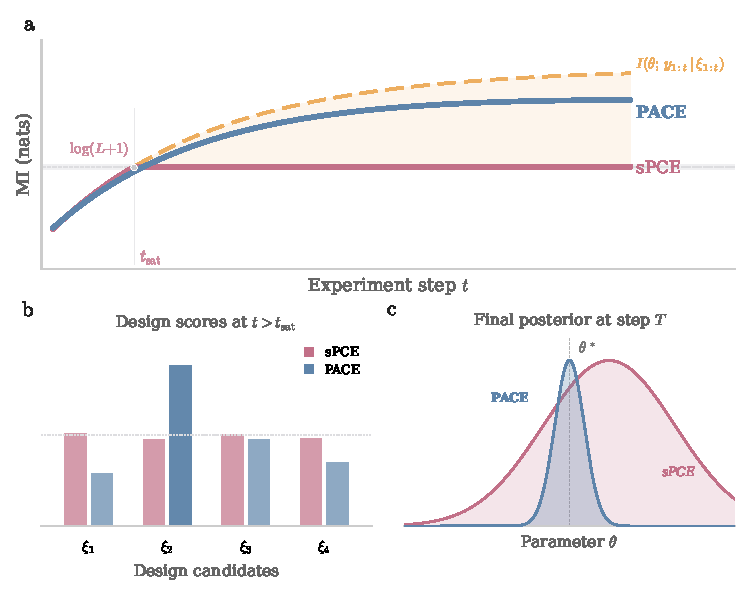
\includegraphics[width=\linewidth]{figures/fig_a1_hero.pdf}
  \caption[The saturation obstacle and the PACE response]{The problem and the response.
  \textbf{(a)} As experiments accumulate, the true information gain keeps rising, but the
  sPCE bound flattens at its $\log(L+1)$ ceiling after a saturation step
  $t_{\mathrm{sat}}$, while PACE continues to track the truth. \textbf{(b)} After
  saturation, sPCE assigns nearly the same score to every candidate design and cannot
  rank them, whereas PACE still separates them. \textbf{(c)} The downstream
  consequence: PACE yields a tighter posterior at the true parameter $\theta^\ast$.}
  \label{fig:hero}
\end{figure}

\section{Research questions}
\label{sec:intro-rqs}

The thesis is organised around one main question and four sub-questions that correspond
to the four contributions.

\medskip
\noindent\textit{Main question: Can sequential Bayesian experimental design be made
feasible and effective on stiff, broad-prior dynamical systems where amortized policy
methods fail?}

\begin{itemize}[leftmargin=*,itemsep=0.2em]
  \item \textbf{RQ1.} When and why does the prior-contrastive sPCE objective, the
  training signal shared by amortized policy methods, fail, and can the failure be
  quantified before any policy is trained?
  \item \textbf{RQ2.} Can a one-time simulation-based posterior estimator supply
  contrastives that escape saturation, and what new cost does this introduce?
  \item \textbf{RQ3.} Does design selection remain valid when the importance weights
  collapse to a single particle?
  \item \textbf{RQ4.} Across a broad suite of systems, when does forward-only
  posterior-contrastive design match or beat amortized policies, and what predicts the
  crossover?
\end{itemize}

\section{Thesis outline}
\label{sec:intro-outline}

Chapter~\ref{sec:related_work} positions PACE against the policy-based,
per-trajectory, and simulation-based-inference literature and states the gap it fills.
Chapter~\ref{sec:methodology} develops the method in full: it sets up sequential BED,
derives the trajectory objective that policy methods optimise and the contrastive
estimators used for evaluation, then presents the saturation diagnosis (RQ1), the PACE
estimator and its cost transfer (RQ2), the analysis of design selection under weight
collapse (RQ3), the forward-only optimiser and its gradient variant, and the evaluation
protocol. Chapter~\ref{sec:results} reports the empirical study on twelve systems
(RQ4), including the ablation that separates the estimator from the optimiser and the
diagnostics that justify trusting the method when the effective sample size is small.
Chapter~\ref{sec:discussion} discusses when PACE should be used, its practical cost,
and its limitations, and Chapter~\ref{sec:conclusion} answers each research question.
Full derivations, system specifications, and additional diagnostics are in the
appendix; the main text is self-contained without it.

        \chapter{Related Work}
\label{sec:related_work}

This thesis sits at the meeting point of three lines of research: Bayesian
experimental design and its amortized variants, simulation-based inference, and the
numerical treatment of stiff differential equations. We review each in enough detail
to make the gap precise. The gap is specific. Amortized policy methods are effective
on standard benchmarks but lose their training signal on stiff, broad-prior systems
with high information per experiment. Per-trajectory methods avoid that failure but
need simulator gradients that stiff systems do not provide reliably. No existing
method uses the current posterior, like the per-trajectory family, while needing
neither a trained policy nor simulator gradients, and while remaining valid when the
posterior is so concentrated that importance weights collapse. We return to this gap
at the end of the chapter.

\section{Bayesian experimental design and the information objective}
\label{sec:rw-bed}

Bayesian experimental design chooses experiments to maximise the expected information
gain (EIG) about unknown parameters~\citep{lindley1956measure,chaloner1995bayesian,ryan2016review}.
For a design $\xi$ and a parameter $\theta$ with prior $p(\theta)$, the EIG is the
mutual information between $\theta$ and the observation $y$,
\begin{equation}
\label{eq:rw-eig}
\mathrm{EIG}(\xi)=I(\theta;y\mid\xi)
=\mathbb{E}_{p(y\mid\xi)}\!\big[H[p(\theta)]-H[p(\theta\mid y,\xi)]\big]
=\mathbb{E}_{p(\theta)p(y\mid\theta,\xi)}\!\left[\log\frac{p(y\mid\theta,\xi)}{p(y\mid\xi)}\right].
\end{equation}
The difficulty is the marginal likelihood $p(y\mid\xi)=\int p(y\mid\theta,\xi)p(\theta)\ud\theta$,
which is intractable for all but the simplest models. Classical estimators use nested
Monte Carlo, drawing an outer sample of $(\theta,y)$ and an inner sample to
approximate the marginal, at a cost that grows with the required
accuracy~\citep{rainforth2018nesting}. In the \emph{sequential} setting the design at
each step depends on the data seen so far, which turns the problem into a control
problem over a growing, history-dependent design space; \citet{rainforth2024modern}
review the modern landscape. The two families that dominate this sequential setting,
and against which PACE is compared, are amortized policies and per-trajectory methods.

\section{Amortized policy-based design}
\label{sec:rw-policy}

\citet{foster2019variational} introduced variational lower bounds on the EIG that can
be optimised by stochastic gradients, and \citet{foster2020unified} unified these into
a single gradient scheme over the prior-contrastive (PCE) family. Deep Adaptive Design
(DAD)~\citep{foster2021deep} made the leap to amortization: rather than optimising a
design at each step, it trains a single policy network $\pi_\phi$ that maps a history
to the next design, by maximising the trajectory mutual information of
Eq.~\eqref{eq:traj-mi}. Because the trajectory marginal is intractable, DAD optimises
the sequential prior-contrastive bound of Eq.~\eqref{eq:traj-spce}, which draws $L$
contrastive parameters from the prior. After training, a design is produced by a
single forward pass, which is what makes the approach attractive for real-time use.
Implicit DAD (iDAD)~\citep{ivanova2021implicit} extended DAD to likelihood-free
models, where the per-step likelihood is unavailable, by using a contrastive bound
estimated from samples, making the method applicable to implicit simulators.

A central fact about all of these methods is that their objective is a contrastive
lower bound on mutual information, and such bounds have a hard ceiling. Any bound
built from $L$ contrastive samples cannot exceed $\log(L+1)$
nats~\citep{mcallester2020formal,paninski2005asymptotic}; the InfoNCE bound that
underlies the contrastive objective makes this explicit, since it is a classification
bound over $L{+}1$ candidates~\citep{oord2018representation,poole2019variational}. This
ceiling is the starting point of our saturation analysis in
Chapter~\ref{sec:methodology}: it is a property of the prior-contrastive objective
itself, not of any particular network or optimiser, so every method in this family
inherits it.

The family is large and active. Step-DAD~\citep{hedman2025stepdad} is semi-amortized:
it pretrains a DAD policy and then finetunes it at each deployment step with a few
gradient updates, trading deployment compute for better designs, and the authors
report instability of pure DAD on the censored-likelihood CES model.
\citet{blau2022optimizing} cast sequential design as a reinforcement-learning problem
and optimise the policy with deep RL, while \citet{huan2016sequential} use approximate
dynamic programming for the same objective. \citet{shen2025vsoed} give a variational
sequential design method trained by RL, and \citet{belliardo2024modelaware} apply
model-aware RL to design in quantum metrology. More recent work amortizes inference
and design jointly: ALINE~\citep{huang2025aline} and the decision-focused method of
\citet{huang2024amortized} train a single network for both posterior inference and
data acquisition, and JADAI~\citep{bracher2025jadai} jointly amortizes adaptive design
and Bayesian inference. For dynamical systems specifically,
\citet{strouwen2026deep} specialise deep adaptive design to model-based design of
experiments for ODEs, and \citet{treloar2022deep} use deep RL to design experiments
for biological ODE models, reporting gains over Fisher-information baselines. All of
these train against the prior-contrastive objective and therefore share its saturation
behaviour on high-information systems.

\section{Per-trajectory and posterior-guided design}
\label{sec:rw-pertraj}

The second family does not train a policy. It maintains an estimate of the current
posterior and chooses the next design by optimising an acquisition score against that
posterior, re-fitting as data arrive. \citet{kleinegesse2020bayesian} estimate the EIG
for implicit models with mutual-information neural estimation and optimise the design
directly. \citet{klein2026supercharging} show that several EIG estimators can be built
on modern simulation-based-inference density estimators and optimised by
multiple-restart gradient ascent through the simulator, unifying inference and design;
this is the closest per-trajectory method to PACE, and the key difference is that it
relies on simulator gradients, whereas PACE uses only forward evaluations.
\citet{iollo2025posterior} and \citet{iollo2025contrastive} develop posterior-guided
and contrastive acquisition criteria, \citet{bharti2024optimizing} optimise designs
through an amortized posterior, and \citet{zaballa2025bridging} bridge sequential
design and simulation-based inference. \citet{vanlier2014bayesian} is an earlier
instance of the same idea for systems-biology ODEs, sequentially selecting informative
conditions by active learning. These methods share PACE's use of the current
posterior; they differ in that they either retrain a proposal each step or depend on
gradients through the simulator.

\section{Simulation-based inference}
\label{sec:rw-sbi}

PACE draws its contrastives from an amortized neural posterior estimator, so it builds
directly on simulation-based inference (SBI), which performs Bayesian inference when
the likelihood is intractable but the simulator can be sampled~\citep{cranmer2020frontier,deistler2025practical}.
Three families are standard. Neural posterior estimation (NPE) parameterises the
posterior $q_\phi(\theta\mid x)$ directly with a conditional density estimator:
\citet{papamakarios2016fast} used mixture density networks,
\citet{lueckmann2017flexible} replaced them with masked autoregressive flows in a
sequential scheme, and \citet{greenberg2019automatic} introduced automatic posterior
transformation (NPE-C) with a correction that keeps the target exact across sequential
rounds. Neural likelihood estimation learns a surrogate likelihood and samples the
posterior with MCMC~\citep{papamakarios2019sequential}, and neural ratio estimation
learns the likelihood-to-evidence ratio by classification~\citep{hermans2020likelihood,durkan2020contrastive,miller2022contrastive}.
The density estimators themselves are usually normalizing
flows~\citep{papamakarios2021normalizing}; we use neural spline
flows~\citep{durkan2019neural} because they give fast, exact density evaluation, which
the importance weighting in PACE requires. More recent flow-matching posterior
estimators~\citep{lipman2023flow,wildberger2024flow,carrasco2026pawsterior} train a
continuous-time velocity field~\citep{chen2018neural} and scale to high dimensions, but
require an ODE solve per density evaluation, which would dominate the per-step cost of
an importance-weighted acquisition score. The \texttt{sbi} toolkit packages these
methods~\citep{tejerocantero2020sbi}, the \texttt{sbibm} suite benchmarks
them~\citep{lueckmann2021benchmarking}, and amortized architectures such as
BayesFlow~\citep{radev2023bayesflow} handle variable numbers of observations.

Two points from this literature matter for PACE. First, sequential SBI methods keep
their importance weights well behaved by retraining the proposal across rounds, for
example with truncated proposals~\citep{deistler2022truncated}; PACE deliberately does
not do this and instead accepts the decline in effective sample size, which is why the
analysis of weight collapse in Chapter~\ref{sec:methodology} is necessary. Second, the
required importance-sampling sample size grows like the exponential of the
Kullback-Leibler divergence between target and proposal~\citep{chatterjee2018sample},
which is the formal reason PACE cannot be read as a calibrated value estimator under a
concentrated posterior. Because amortized posteriors can be miscalibrated, we test
ours with the standard diagnostics: trust and coverage analysis~\citep{hermans2022trust},
simulation-based calibration~\citep{talts2020validating}, distance-to-random-point
coverage~\citep{lemos2023tarp}, and Pareto-smoothed importance
sampling~\citep{vehtari2024pareto}.

\section{Differentiating through stiff simulators}
\label{sec:rw-stiff}

Gradient-based design optimisation, and policy training by the sPCE objective,
differentiate through the ODE solver. On stiff systems this is the dominant cost and a
source of instability. The adjoint method incurs a large compilation overhead and can
be numerically delicate, which has motivated dedicated discretise-then-optimise and
reversible-solver constructions~\citep{kim2024stiff,caldana2025neural,pal2023neural,kidger2024efficient},
and vanishing-gradient pathologies are documented for stiff
dynamics~\citep{linot2025vanishing}. This literature is the practical motivation for
the forward-only optimiser in PACE: by scoring designs with forward simulations only,
PACE avoids the adjoint entirely and applies to stiff and black-box simulators where
gradient-based design is unstable or infeasible.

\section{Classical optimal design for ODE models and model discrimination}
\label{sec:rw-classical}

Before amortization, optimal design for ODE models was dominated by local criteria
based on the Fisher information matrix, such as D-optimality, and by methods for
discriminating between competing models. \citet{huan2014simulation} developed
simulation-based optimal design for nonlinear systems.
\citet{flassig2012optimal} designed optimal stimulus experiments to discriminate
between biochemical ODE models using the overlap of their predictive distributions,
\citet{hainy2022optimal} cast model discrimination as a classification problem and
compared optimal against equidistant designs, and \citet{braniff2022nloed} provide a
software package for nonlinear optimal design in systems biology using the
Jensen-Shannon divergence between predictive densities. These criteria reappear inside
PACE: the collapsed-weight limit of the PACE score reduces to a Fisher-information
criterion (Chapter~\ref{sec:methodology}), which connects the method to this classical
line even though it is derived from a contrastive estimator.

\section{Summary and the gap}
\label{sec:rw-gap}

The amortized policy family casts sequential design as a single trajectory objective
and trains a network to optimise it, but that objective is a prior-contrastive bound
with a $\log(L+1)$ ceiling, so its training signal vanishes on high-information
systems. The per-trajectory family avoids the ceiling by using the current posterior,
but it pays for simulator gradients that stiff systems do not provide reliably, or it
retrains a proposal at every step. Simulation-based inference supplies the posterior
estimator that PACE reuses, but its own theory says the importance weights must
degrade as the posterior concentrates. The gap, then, is a sequential design method
that takes the current posterior from a one-time SBI estimator, scores designs with
forward simulations only, and stays valid when the importance weights collapse. PACE
is that method, and the next chapter derives it.

        \chapter{Methodology}
\label{sec:methodology}

This chapter develops PACE in full. Section~\ref{sec:m-prelim} sets up sequential
design, derives the trajectory objective that policy methods optimise, and presents
the contrastive estimators used for both training and evaluation.
Section~\ref{sec:m-saturation} diagnoses contrastive saturation (RQ1), including the
mechanisms that make it severe on biochemical systems. Section~\ref{sec:m-pace}
defines the PACE estimator and the cost it transfers (RQ2). Section~\ref{sec:m-lowess}
shows why design selection stays valid when the importance weights collapse (RQ3).
Section~\ref{sec:m-forward} gives the forward-only optimiser and its gradient
variant, Section~\ref{sec:m-eval} the evaluation protocol, and
Section~\ref{sec:m-synthesis} draws the four results together.

Everything specific to PACE is derived in this chapter. A few standard results are
stated in the text with full proofs deferred to Appendix~\ref{app:background}.

\section{Background and problem setting}
\label{sec:m-prelim}

\subsection{Sequential design and expected information gain}
\label{sec:m-bed}

A simulator generates an observation $y_t$ from unknown parameters
$\theta\in\Theta$ with prior $p(\theta)$, a design $\xi_t$, and the history
$h_{t-1}=\{(\xi_i,y_i)\}_{i=1}^{t-1}$ of past designs and outcomes (with
$h_0=\varnothing$). We assume two standard ingredients of simulation-based inference
for ODE models with explicit sensor noise: we can draw samples
$y_t\sim p(y_t\mid\theta,\xi_t,h_{t-1})$, and we can evaluate the per-step likelihood
$p(y_t\mid\theta,\xi_t,h_{t-1})$ for a simulated trajectory. The trajectory
likelihood then factorises as
$p(h_t\mid\theta)=\prod_{i=1}^{t}p(y_i\mid\theta,\xi_i,h_{i-1})$.

The value of an experiment is measured by how much it is expected to reduce
uncertainty about $\theta$. The per-step expected information gain (EIG) at $\xi_t$
given the history is the mutual information between $\theta$ and $y_t$ under the
current posterior,
\begin{equation}
\label{eq:step-eig}
I_{h_{t-1}}(\xi_t)
= \mathbb{E}_{p(\theta\mid h_{t-1})\,p(y_t\mid\theta,\xi_t,h_{t-1})}
\!\left[\log\frac{p(y_t\mid\theta,\xi_t,h_{t-1})}{p(y_t\mid\xi_t,h_{t-1})}\right],
\end{equation}
with posterior-predictive marginal
$p(y_t\mid\xi_t,h_{t-1})=\int p(y_t\mid\theta,\xi_t,h_{t-1})\,p(\theta\mid h_{t-1})\,\ud\theta$.
The two readings of this quantity are connected by Bayes' rule. Inside the expectation,
$p(y_t\mid\theta,\xi_t,h_{t-1})/p(y_t\mid\xi_t,h_{t-1})=p(\theta\mid h_t)/p(\theta\mid h_{t-1})$,
so the integrand is the log-ratio of the updated posterior $p(\theta\mid h_t)$ to the
current one. Taking the expectation over $p(\theta\mid h_{t-1})\,p(y_t\mid\theta,\xi_t,h_{t-1})$
and splitting the logarithm turns the two terms into entropies,
\begin{equation}
\label{eq:eig-entropy}
I_{h_{t-1}}(\xi_t)=H[p(\theta\mid h_{t-1})]-\mathbb{E}_{y_t}\,H[p(\theta\mid h_t)],
\end{equation}
the expected drop in posterior entropy from observing $y_t$: the first term is the current
uncertainty, the second is the uncertainty expected to remain after the experiment, and the
design that maximises one form maximises the other. The key feature for
what follows is that both the outer expectation and the denominator use the
\emph{current posterior} $p(\theta\mid h_{t-1})$, which contracts as data accumulate.
Choosing each $\xi_t$ to maximise Eq.~\eqref{eq:step-eig} is the greedy, or myopic,
design rule. PACE follows this rule; the alternative is to learn a policy that
optimises the whole trajectory at once, which we describe next because it is the
method PACE is compared against.

\subsection{From the per-step gain to the policy objective}
\label{sec:m-policy}

A design policy is a function $\pi$ that maps a history to the next design,
$\xi_t=\pi(h_{t-1})$. Running it forward produces a trajectory $h_T$ with likelihood
$p(h_T\mid\theta,\pi)=\prod_{t=1}^{T}p(y_t\mid\theta,\xi_t,h_{t-1})$. Deep Adaptive
Design (DAD) and the methods that follow it train a neural policy $\pi_\phi$ to
maximise the total information gained over the trajectory rather than greedily at
each step~\citep{foster2021deep,ivanova2021implicit}. The total objective is the sum
of the per-step gains, averaged over trajectories, and it simplifies to a single
mutual information. Summing Eq.~\eqref{eq:step-eig} in its entropy form over $t$ and
taking the expectation over trajectories,
\begin{equation}
\label{eq:traj-sum}
\mathcal{I}_T(\pi)=\mathbb{E}\!\Big[\sum_{t=1}^{T} I_{h_{t-1}}(\xi_t)\Big]
=\mathbb{E}\!\Big[\sum_{t=1}^{T}\big(H[p(\theta\mid h_{t-1})]-\mathbb{E}_{y_t}H[p(\theta\mid h_t)]\big)\Big].
\end{equation}
Each intermediate entropy $H[p(\theta\mid h_t)]$ appears twice: once as the starting
entropy of step $t{+}1$, and once inside the inner expectation of step $t$. These two
are not identical random variables, but the tower property
$\mathbb{E}[H[p(\theta\mid h_t)]]=\mathbb{E}\big[\mathbb{E}_{y_{t+1}}H[p(\theta\mid h_{t+1})]\big]$
makes them equal in expectation, so after the outer expectation the sum telescopes,
\begin{equation}
\label{eq:traj-mi}
\mathcal{I}_T(\pi)=H[p(\theta)]-\mathbb{E}\big[H[p(\theta\mid h_T)]\big]
=\mathbb{E}\!\left[\log\frac{p(h_T\mid\theta,\pi)}{p(h_T\mid\pi)}\right],
\end{equation}
the mutual information between $\theta$ and the full trajectory. This is the DAD
training objective~\citep[Theorem~1]{foster2021deep}. Casting the sequential problem
as the single quantity in Eq.~\eqref{eq:traj-mi} is what lets a policy be trained
end to end by gradient ascent, sidestepping the dynamic-programming look-ahead that a
greedy rule ignores. The same objective is used by implicit DAD for likelihood-free
models~\citep{ivanova2021implicit}, by Step-DAD which refines the policy at
deployment~\citep{hedman2025stepdad}, by a reinforcement-learning and value-based
variant~\citep{blau2022optimizing}, by amortized variants
such as vsOED and ALINE~\citep{shen2025vsoed,huang2024amortized,huang2025aline,bracher2025jadai},
and by ODE-specific specialisations~\citep{strouwen2026deep,foster2020unified}. The
obstacle, shared by all of them, is that the trajectory marginal
$p(h_T\mid\pi)=\int p(h_T\mid\theta,\pi)\,p(\theta)\,\ud\theta$ is intractable, which
forces a contrastive estimate.

\subsection{Contrastive estimators: sPCE and sNMC}
\label{sec:m-contrastive}

The contrastive construction replaces the intractable marginal with an average over
$L$ parameters drawn from the prior. With $\theta_0\sim p(\theta)$ generating the
data and contrastives $\theta_{1:L}\sim p(\theta)$, the trajectory sequential
prior-contrastive estimator is
\begin{equation}
\label{eq:traj-spce}
\mathcal{L}_T^{\mathrm{sPCE}}(\pi,L)
=\mathbb{E}\!\left[\log\frac{p(h_T\mid\theta_0,\pi)}{\frac1{L+1}\sum_{\ell=0}^{L}p(h_T\mid\theta_\ell,\pi)}\right]
\le\mathcal{I}_T(\pi),
\end{equation}
a lower bound for every $L$~\citep{foster2021deep}. DAD maximises
Eq.~\eqref{eq:traj-spce} by stochastic gradient ascent, at a cost of $O(L\cdot T)$
simulator solves per gradient step. The per-step analogue, which is the object PACE
estimates and which we use throughout for evaluation, draws $\theta_0,\theta_{1:L}$
the same way and scores
\begin{equation}
\label{eq:spce}
\mathrm{sPCE}_L(\xi_t;h_{t-1})
= \log p(y_t\mid\theta_0,\xi_t,h_{t-1})
- \log\frac{1}{L+1}\sum_{\ell=0}^{L}p(y_t\mid\theta_\ell,\xi_t,h_{t-1}).
\end{equation}
The sequential nested Monte Carlo estimator $\mathrm{sNMC}_L$ uses the same numerator
but divides the denominator sum by $L$ over the contrastives $\theta_{1:L}$ only,
excluding $\theta_0$.

These two estimators bracket the true EIG. The sPCE includes the data-generating
$\theta_0$ in its denominator. Because $\theta_0$ produced $y_t$, the term
$p(y_t\mid\theta_0,\xi_t)$ is systematically large, which inflates the denominator
and pulls the ratio down, so $\mathbb{E}[\mathrm{sPCE}_L]\le I_{h_{t-1}}(\xi_t)$. The
same inclusion caps it: the denominator is at least
$\frac{1}{L+1}p(y_t\mid\theta_0,\xi_t)$, so the ratio is at most $L+1$ and
$\mathrm{sPCE}_L\le\log(L+1)$. Equivalently, sPCE is a classification bound, since
identifying which of the $L{+}1$ exchangeable draws generated $y_t$ has success
probability at most one (Appendix~\ref{app:background}). The sNMC excludes $\theta_0$,
so its denominator is an unbiased estimate of the marginal; by Jensen's inequality
the expected log of an unbiased estimate underestimates the log of the mean, so the
log-marginal is underestimated, the log-ratio overestimated, and
$\mathbb{E}[\mathrm{sNMC}_L]\ge I_{h_{t-1}}(\xi_t)$. Both biases are $O(1/L)$, so
$[\mathrm{sPCE}_L,\mathrm{sNMC}_L]$ brackets the true EIG and tightens as $L\to\infty$.
When one method's sPCE exceeds another's sNMC, the ordering is exact regardless of
estimator bias, a fact we use throughout Chapter~\ref{sec:results}.

\subsection{Amortized neural posterior estimation}
\label{sec:m-npe}

PACE needs samples from the current posterior and the ability to evaluate their
density. Both come from a neural posterior estimator (NPE)
$q_\phi(\theta\mid h_t)\approx p(\theta\mid h_t)$, trained once per system by
simulation-based inference~\citep{cranmer2020frontier,greenberg2019automatic}. We use
a neural spline flow~\citep{durkan2019neural} because it gives fast, exact density
evaluation, which the importance weighting in Section~\ref{sec:m-pace} requires; flow
matching alternatives would require an ODE solve per density
evaluation~\citep{wildberger2024flow}. The flow is conditioned on the history through
a set-equivariant encoder and trained on randomly truncated prefixes, so one network
returns a posterior at every step $t\le T$. Because the training designs are drawn
independently of $\theta$, the network targets the correct posterior for any history,
regardless of how designs are chosen at deployment. Architecture and training are in
Appendix~\ref{app:npe}.

\section{Contrastive saturation}
\label{sec:m-saturation}

This section answers RQ1. We show that sPCE has a hard ceiling, that its gradient
vanishes as the ceiling is reached, that the budget needed to escape grows
exponentially with the information per experiment, and that biochemical systems make
this worse in three identifiable ways.

\subsection{The saturation form and the vanishing gradient}
\label{sec:m-satform}

For an observation $y_t$ generated by $\theta_0$, define the likelihood ratio of
contrastive $\ell$,
\begin{equation}
\label{eq:rratio}
r_\ell = \frac{p(y_t\mid\theta_\ell,\xi_t,h_{t-1})}{p(y_t\mid\theta_0,\xi_t,h_{t-1})}\ge 0,
\qquad \ell=1,\dots,L.
\end{equation}

\begin{lemma}[Saturation form of sPCE]
\label{lem:saturation}
The estimator in Eq.~\eqref{eq:spce} equals
$\mathrm{sPCE}_L(\xi_t;h_{t-1}) = \log(L+1) - \log\!\big(1+\sum_{\ell=1}^{L}r_\ell\big)\le\log(L+1)$,
with equality when $\sum_\ell r_\ell = 0$.
\end{lemma}
\begin{proof}
Factor $p(y_t\mid\theta_0,\xi_t,h_{t-1})$ out of the denominator sum:
$\frac{1}{L+1}\sum_{\ell=0}^{L}p(y_t\mid\theta_\ell,\xi_t,h_{t-1})
= \frac{p(y_t\mid\theta_0,\xi_t,h_{t-1})}{L+1}\big(1+\sum_{\ell=1}^{L}r_\ell\big)$.
Substituting into Eq.~\eqref{eq:spce}, $\log p(y_t\mid\theta_0,\xi_t,h_{t-1})$ cancels
and the constant $L+1$ leaves the logarithm, giving the stated form. Each $r_\ell\ge0$,
so the bound follows.
\end{proof}

Write $S=\sum_{\ell=1}^{L}r_\ell$. Saturation is the regime $S\approx 0$, where
$\mathrm{sPCE}_L\approx\log(L+1)$ for every design. The crucial point for a policy
trained by gradient ascent is that the gradient vanishes together with the value.
Only the second term of the saturation form depends on the design, so
$\nabla_{\xi_t}\mathrm{sPCE}_L=-\nabla_{\xi_t}S/(1+S)$. Writing $r_\ell=e^{\delta_\ell}$
with $\delta_\ell=\log r_\ell$ gives $\nabla_{\xi_t}r_\ell=r_\ell\nabla_{\xi_t}\log r_\ell$,
so
\begin{equation}
\label{eq:grad}
\nabla_{\xi_t}\mathrm{sPCE}_L
= -\frac{\sum_{\ell=1}^{L}r_\ell\,\nabla_{\xi_t}\log r_\ell}{1+\sum_{\ell=1}^{L}r_\ell}.
\end{equation}
The weights in the numerator are the same exponentially small ratios $r_\ell$ that
drive $S\to0$. Assume the log-likelihood-ratio surface is Lipschitz in the design,
$|\nabla_{\xi_t}\log r_\ell|\le C$, which holds for smooth simulators with Lipschitz
observation maps. Bounding the numerator term by term with the triangle inequality,
\begin{equation}
\label{eq:grad-num}
\left|\sum_{\ell=1}^{L} r_\ell\,\nabla_{\xi_t}\log r_\ell\right|
\;\le\; \sum_{\ell=1}^{L} r_\ell\,\bigl|\nabla_{\xi_t}\log r_\ell\bigr|
\;\le\; C\sum_{\ell=1}^{L} r_\ell
\;=\; C\,S ,
\end{equation}
where the first inequality is the triangle inequality, the second uses
$r_\ell\ge0$ together with the Lipschitz bound, and the last is the definition of
$S$. Dividing by the denominator $1+S$ of Eq.~\eqref{eq:grad},
\begin{equation}
\label{eq:grad-bound}
\bigl|\nabla_{\xi_t}\mathrm{sPCE}_L\bigr|
\;=\; \frac{\left|\sum_{\ell=1}^{L} r_\ell\,\nabla_{\xi_t}\log r_\ell\right|}{1+S}
\;\le\; \frac{C\,S}{1+S}
\;\xrightarrow{S\to0}\; 0 .
\end{equation}
Even without the Lipschitz bound, every term in the numerator carries the factor
$r_\ell$, which is exponentially small, so the conclusion is unchanged. This is
stronger than value saturation: not only does every design score about $\log(L+1)$,
but the gradient is near zero everywhere, so the policy receives no direction and its
parameters drift on Monte Carlo noise. Both the objective and its optimisation fail
at once.

\subsection{Why prior contrastives fail}
\label{sec:m-escape}

Saturation happens precisely when a typical prior draw assigns negligible likelihood
to the observed trajectory. To see when, compute the expected contribution of one
contrastive,
\begin{equation}
\label{eq:Er}
\mathbb{E}_{\theta_\ell\sim p(\theta)}[r_\ell]
= \frac{\int p(y_t\mid\theta,\xi_t,h_{t-1})\,p(\theta)\,\ud\theta}{p(y_t\mid\theta_0,\xi_t,h_{t-1})}
= \frac{p^{\mathrm{prior}}(y_t\mid\xi_t,h_{t-1})}{p(y_t\mid\theta_0,\xi_t,h_{t-1})},
\end{equation}
the ratio of the prior-predictive marginal to the likelihood at the truth. We
evaluate it with a Laplace approximation. Take a Gaussian prior
$p(\theta)=\mathcal N(\mu_0,\Sigma_0)$ and observation $y=\mu(\theta,\xi)+\varepsilon$
with $\varepsilon\sim\mathcal N(0,R)$, Fisher information $F=J^\top R^{-1}J$ where
$J=\partial\mu/\partial\theta|_{\theta_0}$, and posterior precision
$\Sigma_{\mathrm{post}}^{-1}=\Sigma_0^{-1}+F$. Expanding the log-likelihood to second
order about $\theta_0$ and completing the square gives a Gaussian integrand, and
integrating yields the marginal
\begin{equation}
\label{eq:laplace-marginal}
p^{\mathrm{prior}}(y\mid\xi)\approx p(y\mid\theta_0,\xi)\,p(\theta_0)\,e^{\frac12 g^\top\Sigma_{\mathrm{post}}g}\,(2\pi)^{d/2}\det(\Sigma_{\mathrm{post}})^{1/2},
\end{equation}
where $g$ is the log-posterior gradient at $\theta_0$. Dividing by
$p(y\mid\theta_0,\xi)$ and keeping the leading volume ratio,
\begin{equation}
\label{eq:escape-scale}
\mathbb{E}[r_\ell]\sim\frac{\det(\Sigma_{\mathrm{post}})^{1/2}}{\det(\Sigma_0)^{1/2}}
=\frac{1}{\det(I+\Sigma_0 F)^{1/2}}=\prod_i(1+\lambda_i)^{-1/2}=e^{-\Lambda},
\qquad \Lambda=\tfrac12\sum_i\log(1+\lambda_i),
\end{equation}
where the $\lambda_i$ are the eigenvalues of $\Sigma_0^{1/2}F\Sigma_0^{1/2}$ (similar
to $\Sigma_0 F$ and hence sharing its eigenvalues) and $\Lambda$ is the
Gaussian-linearised information gain. Appendix~\ref{app:lindley} shows that $\Lambda$ is
exactly the EIG of the linearised experiment (the Bayesian D-optimal value), so the
escape budget grows as $e^{\Lambda}=e^{\mathrm{EIG}}$. The prior-centring and mode-shift
factors omitted from Eq.~\eqref{eq:escape-scale}
contribute $O(d)$ to the exponent and do not change the exponential scaling
(Appendix~\ref{app:lindley}).

The consequence is immediate. The expected sum is $\mathbb{E}[S]=L\,e^{-\Lambda}$, so
by Markov's inequality $\Pr(S\ge1)\le L\,e^{-\Lambda}$. While $L\ll e^{\Lambda}$ the
probability that any contrastive contributes is near zero and saturation is almost
certain; escape requires $L\gtrsim e^{\Lambda}$. The contrastive budget therefore
grows exponentially with the information per experiment. We measure this with the
empirical escape threshold $L_{\mathrm{escape},50}$, the smallest $L$ at which fewer
than half of the rollouts remain within $5\%$ of the $\log(L+1)$ ceiling, evaluated
at random designs as a cheap, method-independent lower bound on the cost.
Table~\ref{tab:escape} reports it for five representative systems against the Laplace
prediction $e^{\Lambda}$.

\begin{table}[t]
\centering\small
\caption[Representative saturation thresholds]{Representative saturation thresholds,
measured at random designs, against the Laplace reference $e^{\Lambda}$. The Laplace
value matches simple systems but understates the threshold once the dynamics are
stiff or far from Gaussian, for the reasons in Section~\ref{sec:m-mechanisms}. The
full twelve-system table is in Appendix~\ref{app:lindley}.}
\label{tab:escape}
\begin{tabular}{lccrrl}
\toprule
System & $d_\theta$ & $d_\xi$ & $\Lambda$ & $e^{\Lambda}$ & $L_{\mathrm{escape},50}$ \\
\midrule
PK 1-comp & 3 & 1 & $1.02$ & $2.8$ & ${\sim}10$ \\
PI3K      & 6 & 2 & $1.49$ & $4.4$ & ${\le}10$ \\
CES       & 4 & 6 & --     & --    & ${\sim}10^4$ \\
ASM1      & 12 & 2 & --    & --    & ${\sim}10^4$ \\
SEIR R=3  & 9 & 9 & $8.64$ & $5{,}648$ & ${>}10^6$ \\
\bottomrule
\end{tabular}
\end{table}

\subsection{Mechanisms that make saturation severe}
\label{sec:m-mechanisms}

The Laplace baseline assumes a Gaussian prior, a quadratic log-likelihood, and a
unimodal posterior. Biochemical ODE systems violate all three, and the measured
threshold then exceeds $e^{\Lambda}$ by one to three orders of magnitude
(Table~\ref{tab:escape}). Three mechanisms explain this, each inflating $|\log r_\ell|$
beyond the Gaussian-quadratic prediction. They are worth stating in the main text
because they tell the experimenter, in advance, which systems will saturate.

\paragraph{Broad priors.}
Prior width enters $\Lambda$ multiplicatively through $\Sigma_0$, since the
eigenvalues $\lambda_i$ of $\Sigma_0^{1/2}F\Sigma_0^{1/2}$ scale with $\Sigma_0$.
Kinetic parameters are routinely assigned log-uniform or log-normal priors spanning
two to four orders of magnitude. A log-uniform prior over $n$ orders of magnitude has
natural-log variance $(n\ln10)^2/12\approx0.44\,n^2$, giving per-parameter prior
eigenvalues of order two to seven for $n=2$ to $4$, which inflate every $\lambda_i$
and hence $\Lambda$. Conversely tight priors ($\pm20\%$) give eigenvalues near
$0.04$, so $\lambda_i\ll1$. This is why PK 8-comp, with calibrated population priors,
has the smallest threshold in Table~\ref{tab:escape-full} despite its twenty
parameters.

\paragraph{High-dynamic-range forward maps.}
The Fisher information $F=J^\top R^{-1}J$ is large when a small parameter change
produces a large change in the output, that is when $\|J\|\gg1$. Stiff kinetics do
exactly this. A Hill function with exponent $n\ge5$ moves between its low and high
states over a narrow parameter range, so $\|J\|$ is large near the transition;
Michaelis-Menten kinetics have peak sensitivity when the substrate is near $K_m$. On
such systems a displacement of about one order of magnitude in parameter space
produces much more than one order of magnitude in observation space, and $F$ turns
this into a large $|\log r_\ell|$.

\paragraph{Non-Gaussian noise.}
The Laplace step assumed Gaussian noise, for which $\log p(y\mid\theta,\xi)$ is
exactly quadratic in the predicted mean $\mu(\theta;\xi)$. Concentration data are
usually modelled with lognormal noise instead, for which (with scale $\sigma$, per
output channel)
\begin{equation}
\label{eq:lognormal-ll}
\log p(y\mid\theta,\xi) = -\frac{1}{2\sigma^2}\bigl(\log y-\log\mu(\theta;\xi)\bigr)^2 - \log\bigl(y\,\sigma\sqrt{2\pi}\bigr).
\end{equation}
The constant $-\log(y\sigma\sqrt{2\pi})$ cancels in the log-ratio $\log r_\ell=\log
p(y\mid\theta_\ell,\xi)-\log p(y\mid\theta_0,\xi)$. Taking the expectation over
$y\sim p(y\mid\theta_0,\xi)$, write $\log y=\log\mu(\theta_0;\xi)+\eta$ with
$\mathbb{E}[\eta]=0$; the cross term in $\eta$ vanishes and, summing over output
channels $k$,
\begin{equation}
\label{eq:lognormal-gap}
\mathbb{E}_y[\log r_\ell] = -\frac{1}{2\sigma^2}\sum_k\bigl(\log\mu^{(k)}(\theta_\ell)-\log\mu^{(k)}(\theta_0)\bigr)^2 .
\end{equation}
Unlike Gaussian noise, whose gap $-\frac{1}{2}\sum_k(\mu^{(k)}(\theta_\ell)-\mu^{(k)}(\theta_0))^2/R_{kk}$
is dominated by the largest-magnitude species, the lognormal gap of
Eq.~\eqref{eq:lognormal-gap} penalises a mismatch at \emph{every} channel equally in
relative (log) terms. On stiff systems whose species span orders of magnitude, the
penalties from all channels accumulate, so $|\log r_\ell|$ is far larger than the
single dominant-species term the Gaussian baseline would predict.

Heteroscedastic Gaussian noise, with a mean-dependent scale
$\sigma(\mu)=\sqrt{(\mu\,\epsilon)^2+\nu^2}$, is worse still. A contrastive that
predicts a different order of magnitude, $\mu(\theta_\ell)\ll\mu(\theta_0)$, has a
narrow noise scale $\sigma(\mu_\ell)\ll\sigma(\mu_0)$, so the residual term
$(y-\mu_\ell)^2/\sigma(\mu_\ell)^2$ diverges because the observed
$y\approx\mu(\theta_0)$ is extreme relative to $\sigma(\mu_\ell)$. The gap again grows
super-quadratically in the mean-level displacement.

\paragraph{Combined effect.}
The three mechanisms compound through a single chain. Under the Gaussian-quadratic
baseline the gap is $|\log r_\ell|\sim(\theta_\ell-\theta_0)^\top F\,(\theta_\ell-\theta_0)$,
which decomposes as $\|\theta_\ell-\theta_0\|^2\cdot\|F\|$. Broad priors (large
$\Sigma_0$) inflate the displacement $\|\theta_\ell-\theta_0\|^2$, since prior draws
land far from $\theta_0$; high-dynamic-range maps inflate $\|F\|=\|J^\top R^{-1}J\|$
through a large Jacobian; and non-Gaussian noise then replaces the quadratic gap with
the larger forms of Eqs.~\eqref{eq:lognormal-gap} above. The amplification is
sequential: broad priors make $\|\theta_\ell-\theta_0\|$ large, high-dynamic-range
maps convert that into a large observation-space displacement, and non-Gaussian noise
converts that displacement into a more negative $\log r_\ell$ than the quadratic
approximation predicts. Systems where several mechanisms are present, such as ASM1 and
SEIR, show the largest gap between $e^{\Lambda}$ and $L_{\mathrm{escape},50}$
(Table~\ref{tab:escape}); systems with Gaussian noise (PK) track the Laplace
prediction; and systems with tight priors (PK 8-comp) have $L_{\mathrm{escape},50}\le10$
regardless of the forward map.

\begin{figure}[t]
  \centering
  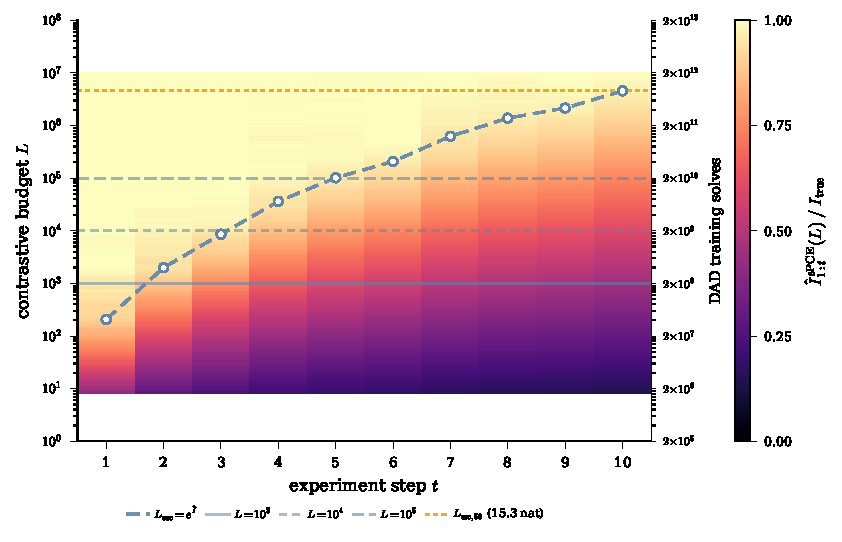
\includegraphics[width=\linewidth]{figures/fig_a1_heatmap.pdf}
  \caption[Escape threshold heatmap]{Contrastive saturation across the benchmark
  suite. Each cell shows $L_{\mathrm{escape},50}$ as a function of the contrastive
  budget $L$. Systems in which the three mechanisms compound (broad priors,
  high-dynamic-range map, non-Gaussian noise) require budgets several orders of
  magnitude above the Laplace prediction $e^{\Lambda}$.}
  \label{fig:heatmap}
\end{figure}

\section{The PACE estimator and the cost transfer}
\label{sec:m-pace}

This section answers RQ2. Prior contrastives fail because they are drawn from a
distribution that is implausible after seeing the data. PACE draws them from an
approximation to the current posterior instead, and corrects the mismatch with
importance weights.

\subsection{Definition}
\label{sec:m-pacedef}


The per-step EIG (Eq.~\eqref{eq:step-eig}) is an expectation under the current posterior of a log-ratio:
\begin{equation}
\label{eq:eig-recall}
I_{h_{t-1}}(\xi_t) = \mathbb{E}_{p(\theta\mid h_{t-1})p(y_t\mid\theta,\xi_t,h_{t-1})}
\left[\log\frac{p(y_t\mid\theta,\xi_t,h_{t-1})}{p(y_t\mid\xi_t,h_{t-1})}\right]
\end{equation}
Estimating this requires two things we do not have in closed form: samples from the current posterior $p(\theta\mid h_{t-1})$ for the outer expectation, and the posterior-predictive marginal $p(y_t\mid\xi_t,h_{t-1})=\int p(y_t\mid\theta,\xi_t,h_{t-1})p(\theta\mid h_{t-1}) d\theta$ in the denominator. The NPE gives an approximation $q_\phi(\theta\mid h_{t-1})\approx p(\theta\mid h_{t-1})$ from which we can sample and whose density we can evaluate. PACE uses importance weighting to bridge the gap. Draw $J$ particles from the NPE, $\theta_{1:J}\sim q_\phi(\theta\mid h_{t-1})$, and assign each an unnormalized importance weight
\begin{equation}
\label{eq:weights}
w_j = \frac{p(\theta_j)p(h_{t-1}\mid\theta_j)}{q_\phi(\theta_j\mid h_{t-1})}
\end{equation}
By Bayes' rule the posterior is $p(\theta_j\mid h_{t-1})=p(\theta_j)p(h_{t-1}\mid\theta_j)/p(h_{t-1})$, so $w_j$ is proportional to the posterior-to-proposal ratio $p(\theta_j\mid h_{t-1})/q_\phi(\theta_j\mid h_{t-1})$, with the unknown evidence $p(h_{t-1})$ as a constant factor across particles. This constant cancels when the weights are normalised,
\begin{equation}
\label{eq:wnorm}
\tilde w_j = \frac{w_j}{\sum_{k=1}^{J}w_k},
\end{equation}
so the normalised weights need only quantities we can compute: the prior $p(\theta_j)$, the trajectory likelihood $p(h_{t-1}\mid\theta_j)$, and the NPE density $q_\phi(\theta_j\mid h_{t-1})$. These weights turn the NPE sample into a weighted approximation of the posterior: for any function $f$, the estimate $$\sum_j\tilde w_jf(\theta_j)\to\mathbb{E}_{p(\theta\mid h_{t-1})}[f(\theta)]$$ as $J\to\infty$. This gives us both missing ingredients. For the outer expectation, the posterior average over $\theta$ is replaced by the weighted sum over particles. For the denominator, the posterior-predictive marginal is the posterior expectation of the likelihood,
\begin{equation}
\label{eq:postpred}
p(y_t\mid\xi_t,h_{t-1})=\mathbb{E}_{p(\theta\mid h_{t-1})}\big[p(y_t\mid\theta,\xi_t,h_{t-1})\big],
\end{equation}
which the weighted particles estimate as $\sum_k\tilde w_k\,p(y_t\mid\theta_k,\xi_t,h_{t-1})$. Substituting both into Eq.~\eqref{eq:eig-recall}: for each particle $\theta_j$, draw an observation $y_{t,j}\sim p(y_t\mid\theta_j,\xi_t,h_{t-1})$. The weighted average over particles approximates the outer expectation, and the weighted likelihood sum approximates the marginal denominator, giving the PACE estimator,
\begin{equation}
\label{eq:pace}
\hat I^{\mathrm{PACE}}(\xi_t;h_{t-1})
= \sum_{j=1}^{J}\tilde w_j
\left[\log p(y_{t,j}\mid\theta_j,\xi_t,h_{t-1})
- \log\sum_{k=1}^{J}\tilde w_k\,p(y_{t,j}\mid\theta_k,\xi_t,h_{t-1})\right].
\end{equation}


Each particle plays two roles: it generates an observation through $y_{t,j}$, and it acts as a weighted contrastive in the denominator for every other particle. The denominator estimates the \emph{posterior}-predictive marginal, which is the correct denominator for the per-step EIG, in contrast to the \emph{prior}-predictive marginal that the saturated sPCE denominator estimates. In implementation we average the bracket over $M$ observation draws per particle.


% PACE is built from self-normalized importance sampling, so we recall the construction before
% applying it. To estimate an expectation $\mathbb{E}_{p}[f(\theta)]$ under a target $p$ from
% which we cannot sample directly, importance sampling draws $\theta_j\sim q$ from a tractable
% proposal and reweights each draw by the ratio $w_j=p(\theta_j)/q(\theta_j)$, since
% $\mathbb{E}_{q}[w\,f]=\mathbb{E}_{p}[f]$. When the target is known only up to a normalising
% constant, as the posterior $p(\theta\mid h)\propto p(\theta)\,p(h\mid\theta)$ is, that
% constant is unknown, but it cancels if the weights are normalised to sum to one: the
% self-normalized estimate $\sum_j\tilde w_j f(\theta_j)$ with $\tilde w_j=w_j/\sum_k w_k$ is
% consistent whenever the proposal covers the target, at the price of an $O(1/J)$ bias. PACE
% applies this idea twice from a single particle set: once to retarget the NPE proposal to the
% current posterior, and once to build the posterior-predictive denominator of the per-step
% EIG from the same particles.

% Draw particles $\theta_{1:J}\sim q_\phi(\theta\mid h_{t-1})$ from the NPE and form
% self-normalized importance weights that retarget the proposal to the posterior,
% \begin{equation}
% \label{eq:weights}
% w_j = \frac{p(\theta_j)\,p(h_{t-1}\mid\theta_j)}{q_\phi(\theta_j\mid h_{t-1})},
% \qquad
% \tilde w_j = \frac{w_j}{\sum_{k=1}^{J}w_k}.
% \end{equation}
% The unnormalized weight is $w_j\propto p(\theta_j\mid h_{t-1})/q_\phi(\theta_j\mid h_{t-1})$,
% the posterior-to-proposal ratio, and the marginal $p(h_{t-1})$ cancels in the
% normalisation, so the weights need only the prior, the trajectory likelihood, and the
% NPE density. For each particle and a candidate design $\xi_t$, draw
% $y_{t,j}\sim p(y_t\mid\theta_j,\xi_t,h_{t-1})$. The PACE estimator is
% \begin{equation}
% \label{eq:pace}
% \hat I^{\mathrm{PACE}}(\xi_t;h_{t-1})
% = \sum_{j=1}^{J}\tilde w_j
% \!\left[\log p(y_{t,j}\mid\theta_j,\xi_t,h_{t-1})
% - \log\sum_{k=1}^{J}\tilde w_k\,p(y_{t,j}\mid\theta_k,\xi_t,h_{t-1})\right].
% \end{equation}
% Each particle plays two roles: it generates an observation through $y_{t,j}$, and it
% acts as a weighted contrastive in the denominator for every other particle. The
% denominator is a self-normalized estimate of the posterior-predictive marginal
% $p(y_t\mid\xi_t,h_{t-1})$, which is the correct denominator for the per-step EIG in
% Eq.~\eqref{eq:step-eig}, in contrast to the prior-predictive marginal that the
% saturated sPCE denominator estimates. In implementation we average the bracket over
% $M$ observation draws per particle. Algebraically Eq.~\eqref{eq:pace} is the per-step
% instance of the importance-weighted contrastive bound whose trajectory form appears
% in the appendices of \citet{foster2021deep} and \citet{ivanova2021implicit}; the
% difference is that $q_\phi$ is trained once by SBI rather than jointly with a policy.

\begin{theorem}[Consistency]
\label{thm:consistency}
If $q_\phi(\cdot\mid h_{t-1})$ supports $p(\cdot\mid h_{t-1})$, the chi-square
divergence $\chi^2(p(\cdot\mid h_{t-1})\,\|\,q_\phi(\cdot\mid h_{t-1}))$ is finite, and
the per-step EIG is finite, then $\hat I^{\mathrm{PACE}}(\xi_t;h_{t-1})\to I_{h_{t-1}}(\xi_t)$
almost surely as $J\to\infty$, with bias $O(1/J)$.
\end{theorem}

This is the standard two-stage self-normalized importance sampling argument: support
inclusion makes the weighted numerator and denominator converge to the posterior
expectations, and finite chi-square gives the $O(1/J)$ rate through the SNIS central
limit theorem (Appendix~\ref{app:pace}). The estimator is decoupled by construction.
The NPE is trained by minimising $-\mathbb{E}_{p(\theta)p(h\mid\theta)}[\log q_\phi(\theta\mid h)]$,
whose gradient is informative no matter how informative the system is, and is then
frozen. This breaks the circular dependence in which a policy and its contrastive
proposal are trained together and both lose signal once sPCE saturates.

\subsection{Relation to ACE, sACE, and sLACE}
\label{sec:m-relation}

The estimator in Eq.~\eqref{eq:pace} shares its algebra with the learned-proposal
contrastive bounds reviewed in Section~\ref{sec:rw-policy}, so being precise about what is
and is not new in PACE matters for its positioning. Recall the lineage of that section:
prior contrastive estimation (PCE, Eq.~\eqref{eq:rw-pce}) draws contrastives from the prior;
adaptive contrastive estimation (ACE, Eq.~\eqref{eq:rw-ace}) draws them from a learned
proposal and reweights each contrastive so the denominator still estimates the marginal,
and is exact for \emph{every} contrastive count when the proposal equals the posterior; and
the sequential forms sACE (Eq.~\eqref{eq:sace}) and sLACE (Eq.~\eqref{eq:slace}) lift ACE to
the trajectory objective but were stated only as unevaluated appendix results in
\citet{foster2021deep} and \citet{ivanova2021implicit}. The exact-when-$q$-is-the-posterior
property of ACE is the static, single-experiment analogue of PACE's perfect-proposal
identity (Section~\ref{sec:m-costtransfer}).

In the sequential bounds the contrastive weight is $p(\theta_\ell)/q(\theta_\ell;h_T)$ and
the proposal conditions on the \emph{full trajectory} $h_T$, so the denominator is an
importance-sampling estimate of the prior marginal
$\int p(h_T\mid\theta,\pi)\,p(\theta)\,\ud\theta=p(h_T\mid\pi)$, the denominator of the
\emph{trajectory} mutual information; setting $q=p(\theta)$ recovers prior contrastives and
the $\log(L+1)$ ceiling. PACE (Eq.~\eqref{eq:pace}) keeps this algebraic shape but makes two
changes: the proposal conditions on the history prefix $h_{t-1}$, and the weight is
$w_j\propto p(\theta_j\mid h_{t-1})/q_\phi(\theta_j\mid h_{t-1})$, so the denominator
estimates the \emph{posterior}-predictive $p(y_t\mid\xi_t,h_{t-1})$ of the per-step EIG
rather than the prior marginal. PACE therefore differs from the sequential bounds
Eqs.~\eqref{eq:sace}-\eqref{eq:slace} in three ways, none of which is in the algebra they
share.
\begin{enumerate}[leftmargin=*,itemsep=0.2em]
  \item \textbf{Target.} sACE and sLACE bound the total trajectory mutual information,
  whose denominator is the prior-marginal under the outer measure $p(\theta)$. PACE
  targets the per-step EIG given history (Eq.~\eqref{eq:step-eig}), whose denominator
  is the posterior-predictive under $p(\theta\mid h_{t-1})$. This retargeting from the
  prior to the running posterior, not the estimator algebra, is the conceptual move,
  and it is what makes the saturation diagnosis and the cost transfer apply.
  \item \textbf{Proposal training.} sACE and sLACE train the proposal jointly with the
  design policy inside the BED objective, which is exactly the circular dependence that
  loses signal when the objective saturates. PACE trains the proposal once, by
  simulation-based inference on simulated pairs (a forward-KL objective), decoupled
  from any design loop, and then freezes it. Online per-step retraining of the
  posterior \citep{klein2026supercharging,zaballa2025bridging} is a different way to
  avoid the prior, at a per-step training cost PACE does not pay.
  \item \textbf{Saturation diagnosis.} The escape threshold $L_{\mathrm{escape}}\approx
  e^{\Lambda}$ (Section~\ref{sec:m-saturation}) and its empirical map across systems
  appear in none of these works; they are what identifies, in advance, the regime in
  which the prior-contrastive objective fails and PACE is needed.
\end{enumerate}
We concede the bound-level overlap plainly: the learned-proposal contrastive estimator
is established prior art in the static case and a proven (if unevaluated) bound in the
sequential case. PACE's contribution rests on the retargeting and the saturation
theory, with the estimator as the vehicle that carries them.

\subsection{The cost transfer: effective sample size}
\label{sec:m-costtransfer}

PACE removes saturation but does not remove the underlying difficulty; it moves it.
Consider a perfect proposal, $q_\phi=p(\theta\mid h)$, and substitute it into
Eq.~\eqref{eq:weights}:
\begin{equation}
\label{eq:widentity}
w_j = \frac{p(\theta_j)\,p(h\mid\theta_j)}{q_\phi(\theta_j\mid h)}\bigg|_{q_\phi=p(\theta\mid h)}
= \frac{p(\theta_j)\,p(h\mid\theta_j)}{p(\theta_j\mid h)}
= \frac{p(\theta_j)\,p(h\mid\theta_j)\,p(h)}{p(\theta_j)\,p(h\mid\theta_j)} = p(h),
\end{equation}
the same constant for every particle, because the posterior is exactly proportional to
the prior times the likelihood. After normalisation $\tilde w_j=1/J$ and the effective
sample size $\mathrm{ESS}=1/\sum_j\tilde w_j^2=J$, its maximum, at any level of
posterior concentration. A perfect proposal therefore never degenerates: a collapse
of the effective sample size signals a proposal mismatch, not concentration alone. In
practice the NPE is imperfect, and as the posterior contracts the mismatch grows; the
effective sample size follows
\begin{equation}
\label{eq:ess}
\mathrm{ESS}\approx\frac{J}{1+\chi^2(p(\theta\mid h)\,\|\,q_\phi(\theta\mid h))},
\end{equation}
which follows from the standard self-normalized identity
$\mathrm{ESS}=(\sum_j w_j)^2/\sum_j w_j^2=J/(1+\widehat{\mathrm{cv}}^2)$, where
$\widehat{\mathrm{cv}}^2$ is the empirical squared coefficient of variation of the weights;
its expectation under the proposal is the chi-square divergence
$\mathbb{E}_{q_\phi}[(p/q_\phi-1)^2]=\chi^2(p\,\|\,q_\phi)$. The effective sample size
declines as the posterior tightens. That this $\chi^2$ is finite at all, which the
bias rate of Theorem~\ref{thm:consistency} requires, is itself due to the likelihood
factor in the weight: it cancels the divergence that a prior-targeting weight would
incur (Appendix~\ref{app:chi2}). This is the same concentration that caused saturation,
now appearing as weight degeneracy: the burden has moved from policy training to
amortized inference. Reliable estimation of the EIG \emph{value} under a
collapsed weight set would need a number of particles growing like
$e^{D_{\mathrm{KL}}(p\,\|\,q_\phi)}$~\citep{chatterjee2018sample}, which is infeasible
for our systems. Design selection, however, needs reliable \emph{rankings}, not
values, and the next section shows the rankings survive.

\begin{figure}[t]
  \centering
  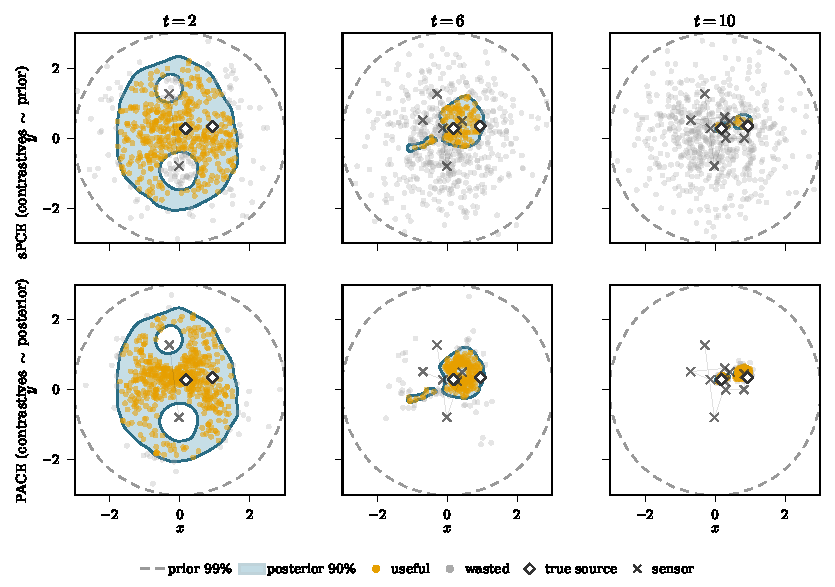
\includegraphics[width=0.8\linewidth]{figures/fig_a1_contraction.pdf}
  \caption[Posterior contraction and ESS collapse]{Posterior contraction and
  effective sample size across BED steps. As the posterior concentrates, the
  proposal mismatch grows and the ESS collapses, yet the per-step information
  $\Delta S_t$ remains positive and the design ranking is preserved.}
  \label{fig:contraction}
\end{figure}

\section{Design selection under weight collapse}
\label{sec:m-lowess}

This section answers RQ3. We derive a decomposition of the PACE score that separates a
design-independent part from the part that ranks designs, show that the collapsing
weight scale enters only the design-independent part, and identify the limiting
criterion.

\subsection{Decomposition into weight entropy and a design-dependent term}
\label{sec:m-decomp}

Define the cross-particle likelihood ratio
$r_{k\leftarrow j}(\xi_t)=p(y_{t,j}\mid\theta_k,\xi_t)/p(y_{t,j}\mid\theta_j,\xi_t)$,
with $r_{j\leftarrow j}=1$, and the competitor ratio
$\Psi_j(\xi_t)=\sum_{k\ne j}(w_k/w_j)\,r_{k\leftarrow j}(\xi_t)$. Starting from
Eq.~\eqref{eq:pace}, substitute $\tilde w_k=w_k/W$ with $W=\sum_k w_k$ and factor
$p(y_{t,j}\mid\theta_j,\xi_t)$ out of the inner sum. For the $j$-th term,
\[
\log p(y_{t,j}\mid\theta_j,\xi_t)-\log\!\sum_k w_k\,p(y_{t,j}\mid\theta_k,\xi_t)+\log W
= \log W-\log w_j-\log\!\big[1+\Psi_j(\xi_t)\big],
\]
where the likelihood of the generating particle cancels and the $k{=}j$ term is split
off using $r_{j\leftarrow j}=1$. Taking the weighted sum over $j$ and using
$\sum_j\tilde w_j\log w_j=\sum_j\tilde w_j\log\tilde w_j+\log W=-H(\tilde w)+\log W$,
the $\log W$ terms cancel and
\begin{equation}
\label{eq:decomp}
\hat I^{\mathrm{PACE}}(\xi_t)
= \underbrace{H(\tilde w)}_{\text{constant in }\xi_t}
- \underbrace{\sum_j \tilde w_j\log\big[1+\Psi_j(\xi_t)\big]}_{\bar\Phi(\xi_t)},
\end{equation}
with $H(\tilde w)=-\sum_j\tilde w_j\log\tilde w_j$ the entropy of the weights. The
weight entropy does not depend on the design, so
\begin{equation}
\label{eq:argmax}
\arg\max_{\xi_t}\hat I^{\mathrm{PACE}}(\xi_t)=\arg\min_{\xi_t}\bar\Phi(\xi_t).
\end{equation}

\subsection{The collapsed-weight limit}
\label{sec:m-collapse}

Now take the limit $\mathrm{ESS}\to1$, in which one weight dominates,
$\tilde w_{\mathrm{dom}}\to1$ and $\tilde w_j\to0$ for $j\ne\mathrm{dom}$. The
design-dependent term reduces to a single summand,
$\bar\Phi(\xi_t)\to\log[1+\Psi_{\mathrm{dom}}(\xi_t)]$. Since $\tilde w_{\mathrm{dom}}\to1$
forces $w_k/w_{\mathrm{dom}}\to0$ for every other $k$, we have
$\Psi_{\mathrm{dom}}(\xi_t)\to0$. Because $x\mapsto\log(1+x)$ is increasing,
$\arg\min_{\xi_t}\log[1+\Psi_{\mathrm{dom}}]=\arg\min_{\xi_t}\Psi_{\mathrm{dom}}$ holds
exactly, and the first-order expansion $\log(1+x)\approx x$ gives the interpretable
criterion
\begin{equation}
\label{eq:lr-limit}
\arg\max_{\xi_t}\hat I^{\mathrm{PACE}}(\xi_t)
= \arg\min_{\xi_t}\sum_{k\ne\mathrm{dom}}\frac{w_k}{w_{\mathrm{dom}}}\,r_{k\leftarrow\mathrm{dom}}(\xi_t).
\end{equation}
PACE selects the design that best separates the dominant particle from its
competitors, with fixed weights $w_k/w_{\mathrm{dom}}$. The monotone identity
$\arg\min_{\xi_t}\log[1+\Psi_{\mathrm{dom}}]=\arg\min_{\xi_t}\Psi_{\mathrm{dom}}$ is exact
for a single realised $y_{t,\mathrm{dom}}$; with $M{>}1$ observation draws per particle,
Algorithm~\ref{alg:ftk} ranks designs by the mean of $\log[1+\Psi_{\mathrm{dom}}(\xi_t)]$
over draws, which is the faithful scored objective and reduces to the weighted-ratio
form of Eq.~\eqref{eq:lr-limit} only at $M{=}1$.

\subsection{Common-mode cancellation}
\label{sec:m-cancellation}

Equation~\eqref{eq:lr-limit} is the validity argument. Under a collapsed weight set the
unnormalized weights can be astronomically large, which makes the PACE \emph{value} an
unreliable estimate of the EIG. The \emph{ranking} is protected for two reasons.
First, the weight entropy $H(\tilde w)$ in the decomposition~\eqref{eq:decomp} is
identical across candidate designs and drops out. Second, inside $\bar\Phi(\xi_t)$ the
weights $\tilde w_j$ and the ratios $w_k/w_j$ are fixed by the particle bank; only the
likelihood ratios $r_{k\leftarrow j}(\xi_t)$ change with the design. The diverging
weight scale therefore enters only design-independent terms and cancels in the
ranking. This guards the ranking against the weight scale; it does not reduce Monte
Carlo variance, which we measure directly in Chapter~\ref{sec:results}.

The two regimes are joined smoothly by the single estimator. When the effective
sample size is high, $\bar\Phi$ is a well-resolved weighted average and PACE
approximates the EIG with $O(1/J)$ bias. As the weights concentrate, $\bar\Phi$
deforms continuously into the single-particle form, with no threshold and no mode
switch. In that limit, if one competitor $\theta_{k^\ast}$ dominates the rest, the
criterion becomes a pairwise log likelihood-ratio test, and its expectation over the
generated $y_{t,\mathrm{dom}}$ is the Kullback-Leibler divergence between the two
predictive distributions,
\begin{equation}
\label{eq:kl}
\mathbb{E}_{y_{t,\mathrm{dom}}}\!\left[\log\frac{p(y_{t,\mathrm{dom}}\mid\theta_{\mathrm{dom}},\xi_t)}{p(y_{t,\mathrm{dom}}\mid\theta_{k^\ast},\xi_t)}\right]
= D_{\mathrm{KL}}\!\big(p(y_t\mid\theta_{\mathrm{dom}},\xi_t)\,\|\,p(y_t\mid\theta_{k^\ast},\xi_t)\big).
\end{equation}
For Gaussian likelihoods with a linearised forward map, the two predictive means differ by
the design Jacobian acting on $\theta_{\mathrm{dom}}-\theta_{k^\ast}$, so the Gaussian KL of
Eq.~\eqref{eq:kl} reduces to the quadratic form
$\tfrac12(\theta_{\mathrm{dom}}-\theta_{k^\ast})^\top F(\xi_t)(\theta_{\mathrm{dom}}-\theta_{k^\ast})$,
where $F(\xi_t)$ is the Fisher information of the design. Treating $\theta_{k^\ast}$ as a
posterior draw with covariance $\Sigma_{\mathrm{post}}$ and taking the expectation over it
gives, through $\mathbb{E}[(\theta_{\mathrm{dom}}-\theta_{k^\ast})(\theta_{\mathrm{dom}}-\theta_{k^\ast})^\top]=\Sigma_{\mathrm{post}}$
(which holds exactly when $\theta_{\mathrm{dom}}$ equals the posterior mean; in practice
the dominant particle approximates the mode, so this step is a Laplace-level approximation),
the expected criterion
$\tfrac12\,\mathrm{tr}\!\big(F(\xi_t)\Sigma_{\mathrm{post}}\big)$: Fisher information weighted
by residual posterior uncertainty, which is the D-optimal and classical Fisher design
objective of Section~\ref{sec:rw-classical}. This is the trace form of the
Gaussian-linearised EIG, so the quantity $\Lambda$ that drove saturation in
Section~\ref{sec:m-saturation} reappears here as the design objective; the underlying Laplace
linearisation is derived in full in Appendix~\ref{app:lindley}.

\subsection{Failure modes}
\label{sec:m-failure}

Two situations make the criterion uninformative. If the parameter differences between
the dominant particle and its competitors lie in directions that no design can
resolve, that is in or near the null space of $F(\xi_t)$ for all competitors and all
candidate designs, then Eq.~\eqref{eq:lr-limit} is flat and carries only noise.
Maximising a flat, noisy criterion can do slightly worse than uniform sampling, which
at least spreads coverage. This is an identifiability plateau, and the Goodwin
oscillator in Chapter~\ref{sec:results} is an example. Separately, if the NPE places
its mass in a region disjoint from the true posterior, the dominant particle is far
from the truth and PACE optimises designs to separate wrong hypotheses from each
other. This mode collapse is detectable through the diagnostics of
Section~\ref{sec:m-eval} (a diverging Pareto shape of the weights, raw coverage going
to zero), and we find no evidence of it on our systems, which is expected for the
unimodal posteriors of well-observed ODE systems.

\section{Forward-only design optimisation}
\label{sec:m-forward}

The reason to pair PACE with a forward-only optimiser is the same reason policy
training is expensive on the systems that motivate this work. A policy gradient
differentiates the sPCE objective with respect to the design, and therefore through
the simulator, by an adjoint pass. Each training iteration simulates $L$ contrastive
trajectories of $T$ steps forward and then backpropagates through all $L\cdot T$
solves. On stiff systems the backward pass is substantially more expensive than the
forward pass and carries a large fixed adjoint-compilation overhead~\citep{kim2024stiff,pal2023neural,caldana2025neural}.
Moreover, on saturated systems $L$ must reach $L_{\mathrm{escape},50}$ before the
gradient carries any signal at all (Section~\ref{sec:m-saturation}), so the total
training cost is $O(N_{\mathrm{iter}}\cdot L_{\mathrm{escape},50}\cdot T)$
forward-plus-backward solve pairs. For SEIR R=3, with $L_{\mathrm{escape},50}>10^6$ and
$T=10$, this exceeds $10^{10}$ solve pairs; for ASM1, with $L_{\mathrm{escape},50}\sim10^4$
and a stiff integrator, the adjoint overhead makes policy training infeasible in our
infrastructure. PACE removes the backward pass entirely. The NPE is trained without
differentiating through the simulator, and at deployment designs are chosen by search.

\subsection{Forward-only search}
\label{sec:m-ftk}

Algorithm~\ref{alg:ftk} draws the particle bank once per step, samples candidate
designs, scores each with PACE, and optionally refines the pool with one or more
cross-entropy rounds~\citep{rubinstein2004cross}. The per-step cost is
$J\big(1+M(1+C)N_{\mathrm{cand}}\big)$ forward solves: $J$ to weight the particles
against the history once, and $M$ observation draws for each of the
$(1+C)N_{\mathrm{cand}}$ scored candidates. There is no backward pass and no
differentiable simulator, so the method applies to stiff and black-box simulators.
Common-mode cancellation (Section~\ref{sec:m-cancellation}) guarantees that the search
optimises the correct ranking even when the effective sample size has collapsed.

\begin{algorithm}[t]
\caption{Forward-only design search (PACE-ftk) at step $t$}
\label{alg:ftk}
\begin{algorithmic}[1]
\Require history $h_{t-1}$, NPE $q_\phi$, particles $J$, draws $M$, candidates
$N_{\mathrm{cand}}$, rounds $C$, elite fraction $\rho$
\State draw $\theta_{1:J}\sim q_\phi(\theta\mid h_{t-1})$ and compute
$\tilde w_{1:J}$ by Eq.~\eqref{eq:weights}
\State sample $\{\xi^{(k)}\}_{k=1}^{N_{\mathrm{cand}}}\sim\mathrm{Uniform}(\Xi)$
\For{$k=1,\dots,N_{\mathrm{cand}}$}
  \State score $\hat I^{(k)}\gets\frac1M\sum_{m=1}^{M}\hat I^{\mathrm{PACE}}(\xi^{(k)})$ by Eq.~\eqref{eq:pace} \Comment{$JM$ forward solves}
\EndFor
\For{$c=1,\dots,C$}
  \State fit a Gaussian to the top $\lceil\rho N_{\mathrm{cand}}\rceil$ designs; resample $N_{\mathrm{cand}}$, clip to $\Xi$, rescore
\EndFor
\State \Return the best-scoring design over the whole pool
\end{algorithmic}
\end{algorithm}

\subsection{Gradient variant}
\label{sec:m-grad}

On systems where the simulator gradient is reliable, the PACE score can also be
optimised by gradient ascent. We call this variant PACE-grad
(Algorithm~\ref{alg:grad}). It differs from a policy method in a crucial way: it
differentiates through the simulator only at \emph{deployment}, to refine a single
design, not during a costly training loop, and it never relies on the saturated sPCE
signal. It warm-starts from the best of $N_{\mathrm{cand}}$ random candidates and runs
a few Adam steps from each of $R$ restarts. We include it to separate the contribution
of the estimator from that of the optimiser: PACE-ftk and PACE-grad share the same
one-time NPE proposal and candidate budget, so comparing them isolates the optimiser
(Chapter~\ref{sec:results}). Gradient ascent helps where the gradient is informative
and hurts on stiff systems where it is not, which is the empirical case for the
forward-only default.

\begin{algorithm}[t]
\caption{Gradient design search (PACE-grad) at step $t$}
\label{alg:grad}
\begin{algorithmic}[1]
\Require history $h_{t-1}$, NPE $q_\phi$, particles $J$, draws $M$, warm pool
$N_{\mathrm{cand}}$, restarts $R$, Adam steps $K$, step size $\eta$
\State draw $\theta_{1:J}\sim q_\phi(\theta\mid h_{t-1})$ and compute $\tilde w_{1:J}$
\State sample $N_{\mathrm{cand}}$ candidates, score by Eq.~\eqref{eq:pace}, keep the top $R$ as warm starts $\{\xi^{(r)}_0\}$
\For{$r=1,\dots,R$}
  \For{$k=1,\dots,K$}
    \State $\xi^{(r)}_{k}\gets\mathrm{clip}_\Xi\!\big(\xi^{(r)}_{k-1}+\eta\,\nabla_{\xi}\,\tfrac1M\textstyle\sum_m\hat I^{\mathrm{PACE}}(\xi^{(r)}_{k-1})\big)$ \Comment{adjoint through the simulator}
  \EndFor
\EndFor
\State \Return the best-scoring design among $\{\xi^{(r)}_{K}\}_{r=1}^{R}$
\end{algorithmic}
\end{algorithm}

\section{Evaluation protocol}
\label{sec:m-eval}

We evaluate every method on the same prior-contrastive scale. For each rollout we
report the bracket $[\mathrm{sPCE}_L,\mathrm{sNMC}_L]$, computed on the same rollouts
at the same $L$, which bounds the true mean EIG from below and above. These estimators
use the prior $p(\theta)$ in their denominator, so they bound the prior-contrastive
per-step gain, the common, method-agnostic scale shared by PACE, DAD, and random and
the one on which the saturation analysis operates. This is not the posterior-conditional
per-step EIG of Eq.~\eqref{eq:step-eig} that PACE's own estimator targets; the two
coincide at $t{=}1$ (empty history) and are reconciled step by step by the chain-rule
increments $\Delta S_t$ introduced below. When one method's lower bound exceeds
another's upper bound by more than the combined standard error, the ordering is
definitive and no estimation slack can reverse it. All main
comparisons use $n=300$ paired rollouts, three data-generating seeds of one hundred
each, with paired tests, since small-sample sPCE estimates are unreliable.

To see where information is acquired within a rollout, we also report the per-step
increment $\Delta S_t=S_t-S_{t-1}$, where $S_t$ is the sPCE on the length-$t$ prefix.
These increments telescope to the trajectory sPCE (Appendix~\ref{app:background}) and
show how much each step contributes as the posterior contracts. Because PACE is
deployed with a collapsing effective sample size, we report four diagnostics that each
rule out a specific failure: bootstrap pick-stability, raw versus importance-resampled
posterior coverage, per-step simulation-based calibration, and the Pareto shape of the
weights. These are developed with the results in Chapter~\ref{sec:results} and in full
in Appendix~\ref{app:diagnostics}. The suite of twelve systems is specified in
Appendix~\ref{app:systems}.

\section{Synthesis: one quantity, four roles}
\label{sec:m-synthesis}

The four results are linked by the likelihood ratio $r$ and its prior average
$e^{-\Lambda}$. In Section~\ref{sec:m-saturation}, $\mathbb{E}[r]\sim e^{-\Lambda}$ is
what drives sPCE to its ceiling, vanishes its gradient, and makes the escape budget
grow as $e^{\Lambda}$. In Section~\ref{sec:m-pace}, the same concentration that shrinks
$\mathbb{E}[r]$ reappears as the chi-square divergence in Eq.~\eqref{eq:ess} and
collapses the effective sample size; PACE removes the saturation but inherits this as
the cost of amortized inference. In Section~\ref{sec:m-lowess}, under that collapse the
design criterion reduces to a weighted sum of the same ratios $r$
(Eq.~\eqref{eq:lr-limit}) and approaches the Fisher value $\Lambda$ in a new role, now
the objective rather than the obstacle (Eq.~\eqref{eq:kl}). Chapter~\ref{sec:results}
closes the loop: the crossover between PACE and the policy is predicted by the
saturation threshold, the $\Lambda$ side of this object, and not by the effective
sample size, the chi-square side. One quantity therefore explains why prior
contrastives fail, how PACE fixes it, why the fix stays valid under its own cost, and
when the method wins.

        \chapter{Results}
\label{sec:results}

This chapter answers RQ4. Section~\ref{sec:r-saturation} measures saturation across
the suite, confirming the diagnosis of Section~\ref{sec:m-saturation}.
Section~\ref{sec:r-toy} isolates the estimator on a controlled toy.
Section~\ref{sec:r-anchors} reports the head-to-head on the systems where saturation
bites, and Section~\ref{sec:r-cross} on the systems where it does not.
Section~\ref{sec:r-ablation} is the ablation study: it separates the contribution of
the estimator from that of the optimiser. Section~\ref{sec:r-perstep} reads the
rollouts step by step and shows that performance is not predicted by the effective
sample size, and Section~\ref{sec:r-diag} reports the diagnostics that justify
trusting the method when that sample size is small.

All numbers are from the validated result set. Each main comparison uses $n=300$
paired rollouts, with the sPCE lower bound and sNMC upper bound on the same rollouts
at the same budget $L_{\mathrm{eval}}$. A dagger ($\dagger$) marks a definitive
ordering, where one method's lower bound exceeds the other's upper bound by more than
the combined standard error.

\section{Saturation across the suite}
\label{sec:r-saturation}

Figure~\ref{fig:lscan} shows the saturation transition for five representative
systems as the contrastive budget grows. The two low-information systems, PI3K and
Monod, escape the ceiling by $L\approx30$. The Goodwin oscillator, with stiff Hill
kinetics, escapes only near $L\approx10^4$. SEIR R=3 has not escaped even at $L=10^6$,
which is an order of magnitude beyond the $L=10^5$ budget at which policy methods are
usually trained. The measured escape thresholds span more than five orders of
magnitude (Table~\ref{tab:escape}; Appendix~\ref{app:lindley}). The Gaussian
prediction $e^{\Lambda}$ matches the simplest systems but understates the threshold by
one to three orders of magnitude once the dynamics are stiff or far from Gaussian, the
behaviour predicted by the three mechanisms in Section~\ref{sec:m-mechanisms}. This is
the empirical content of RQ1: the failure is real, it is system-dependent, and it can
be screened for in advance with a cheap random-design scan.

\begin{figure}[t]
  \centering
  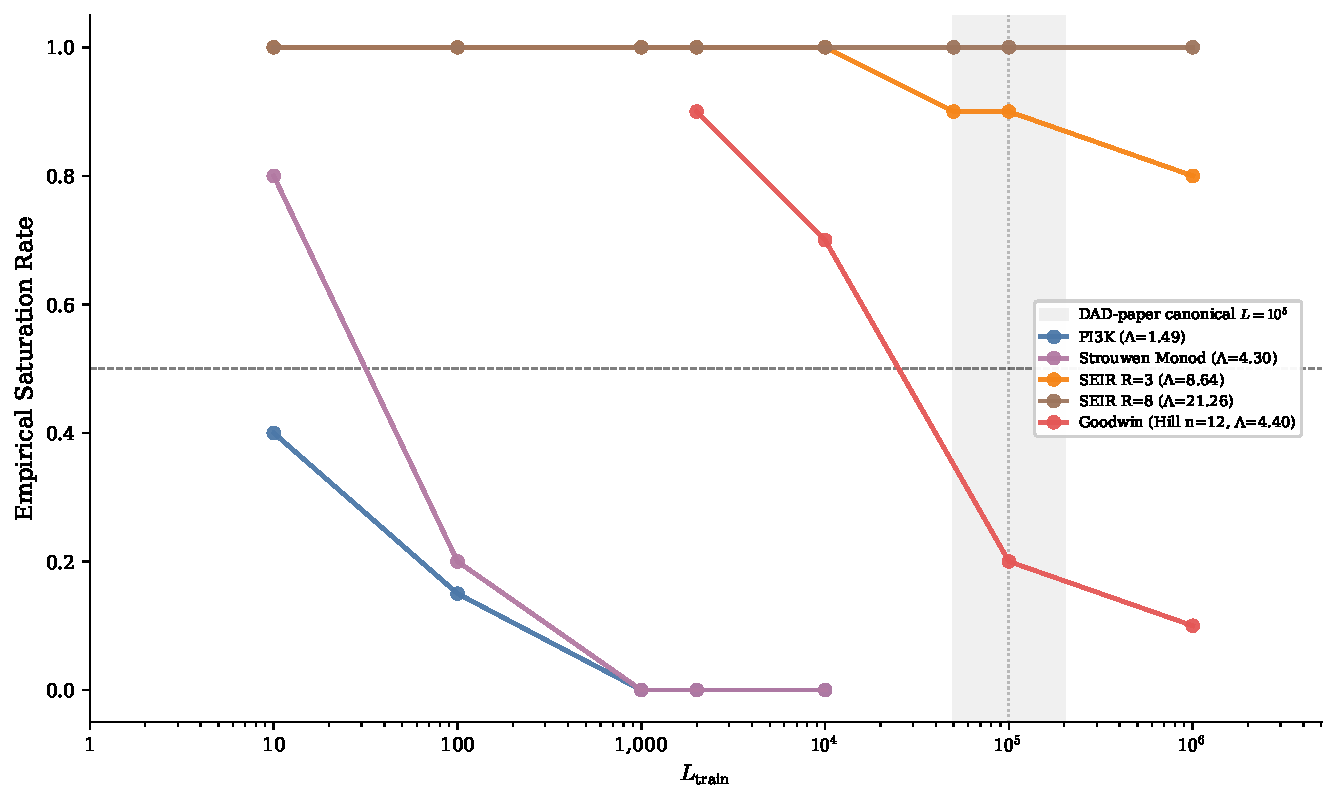
\includegraphics[width=0.78\linewidth]{figures/fig3_lscan_transitions.pdf}
  \caption[Empirical saturation transitions]{Empirical saturation rate against the
  contrastive budget $L$ for five representative systems. PI3K and Monod escape by
  $L\approx30$; the Goodwin oscillator escapes near $L\approx10^4$; SEIR R=3 remains
  at the ceiling across the scan. The shaded band marks the $L=10^5$ budget at which
  policy methods are typically trained.}
  \label{fig:lscan}
\end{figure}

\section{Removing the saturation bias on a controlled toy}
\label{sec:r-toy}

To separate the estimator from the optimiser, we use a controlled six-dimensional
Michaelis-Menten cascade with a prior spanning four orders of magnitude. We sweep the
number of NPE training simulations $N_{\mathrm{NPE}}$ from $10^2$ to $5\times10^4$,
train a fresh posterior estimator in each cell, and evaluate both estimators on
held-out targets at a fixed budget. Figure~\ref{fig:toy} shows the expected phase
transition. The prior-contrastive estimator stays pinned at its ceiling, about six
nats above the true EIG, for every value of $N_{\mathrm{NPE}}$, because no amount of
posterior-estimator training changes where the prior contrastives are drawn from. PACE
descends to the true EIG once the proposal is accurate enough, between
$N_{\mathrm{NPE}}=500$ and $5000$. Since the optimiser is identical in both arms, the
improvement is due to replacing prior contrastives with posterior ones, which is the
core of the cost transfer (RQ2).

\begin{figure}[t]
  \centering
  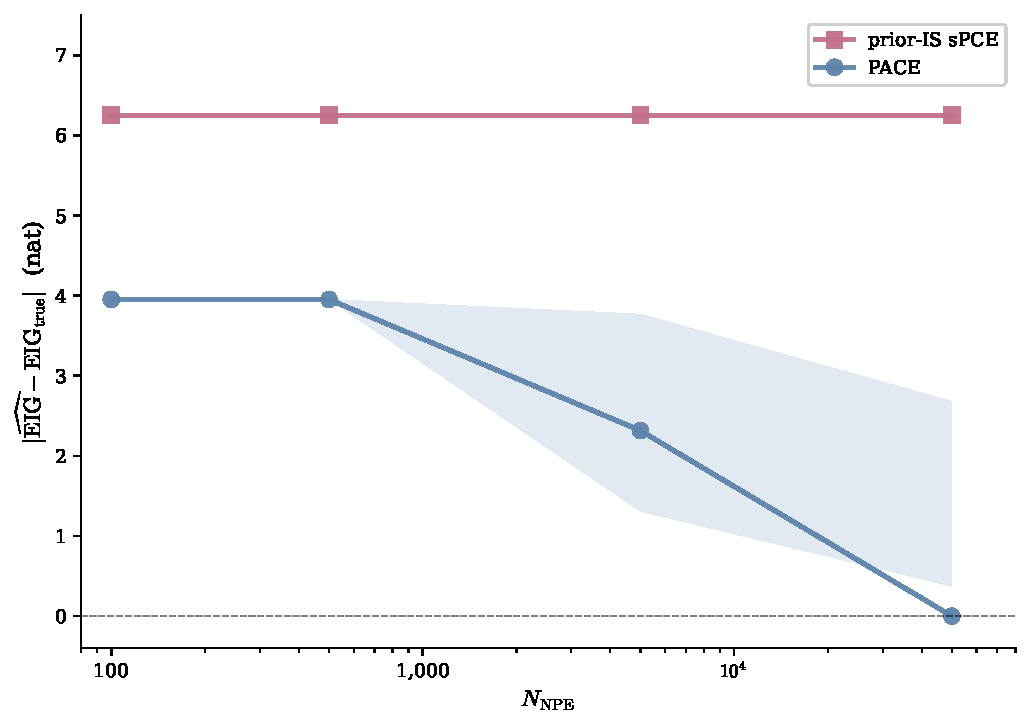
\includegraphics[width=0.6\linewidth]{figures/fig4a_eig_convergence.pdf}
  \caption[Estimator convergence on the controlled toy]{On a six-dimensional
  Michaelis-Menten cascade, PACE converges to the true EIG as the NPE training budget
  $N_{\mathrm{NPE}}$ grows, while the prior-contrastive estimator stays at the
  saturation ceiling regardless of $N_{\mathrm{NPE}}$.}
  \label{fig:toy}
\end{figure}

\section{Anchor systems: where saturation bites}
\label{sec:r-anchors}

Table~\ref{tab:results} is the main comparison against DAD and random design, and
Table~\ref{tab:results-rand} covers the two systems for which no DAD comparator is
available. We read the saturated anchors here and the unsaturated systems in
Section~\ref{sec:r-cross}.

\begin{table}[t]
\centering\footnotesize
\setlength{\tabcolsep}{4pt}
\caption[Per-step EIG bounds: PACE versus DAD and random]{Per-step EIG bounds for
PACE (forward-only), DAD, and random design. Each cell is the mean $\pm$ SEM over $n=300$
rollouts; lower bound ($\uparrow$) is sPCE, upper bound ($\downarrow$) is sNMC.
$\Delta_{\mathrm{sPCE}}$ is the paired PACE${-}$DAD difference $\pm$ SEM with its $t$-test
$p$-value; $\dagger$ marks a definitive ordering. ASM1 and Goodwin are in
Table~\ref{tab:results-rand}.}
\label{tab:results}
\begin{tabular}{lcccccc c}
\toprule
& \multicolumn{2}{c}{PACE} & \multicolumn{2}{c}{DAD} & \multicolumn{2}{c}{Random} & \\
\cmidrule(lr){2-3}\cmidrule(lr){4-5}\cmidrule(lr){6-7}
System ($L_{\mathrm{eval}}$) & Lower bound\,$\uparrow$ & Upper bound\,$\downarrow$ & Lower bound\,$\uparrow$ & Upper bound\,$\downarrow$ & Lower bound\,$\uparrow$ & Upper bound\,$\downarrow$ & $\Delta_{\mathrm{sPCE}}$ ($p$) \\
\midrule
CES ($10^7$)        & $12.98{\pm}0.22$ & $15.37{\pm}0.41$ & $12.05{\pm}0.14$ & $12.17{\pm}0.15$ & $9.01{\pm}0.31$ & $11.11{\pm}0.53$ & $+0.93{\pm}0.18$ ($3.6\mathrm{e}{-}7$)$^\dagger$ \\
SEIR R=3 ($10^7$)   & $14.78{\pm}0.09$ & $16.85{\pm}0.27$ & $7.47{\pm}2.40$ & $9.34{\pm}2.44$ & $14.16{\pm}0.11$ & $15.42{\pm}0.24$ & $+7.31{\pm}2.41$ ($2.6\mathrm{e}{-}3$)$^\dagger$ \\
Monod ($5{\times}10^3$) & $5.28{\pm}0.06$ & $5.35{\pm}0.07$ & $5.94{\pm}0.06$ & $6.07{\pm}0.07$ & $4.77{\pm}0.06$ & $4.81{\pm}0.06$ & $-0.66{\pm}0.07$ ($3.2\mathrm{e}{-}17$)$^\dagger$ \\
\midrule
Src.\ loc.\ $p{=}2$ ($10^5$) & $9.12{\pm}0.11$ & $9.83{\pm}0.18$ & $7.60{\pm}0.11$ & $7.73{\pm}0.13$ & $4.63{\pm}0.12$ & $4.65{\pm}0.12$ & $+1.52{\pm}0.15$ ($3.9\mathrm{e}{-}20$)$^\dagger$ \\
Src.\ loc.\ $p{=}5$ ($10^5$) & $9.84{\pm}0.11$ & $11.89{\pm}0.27$ & $8.77{\pm}0.13$ & $9.42{\pm}0.20$ & $4.19{\pm}0.15$ & $4.22{\pm}0.15$ & $+1.07{\pm}0.18$ ($5.8\mathrm{e}{-}9$)$^\dagger$ \\
Src.\ loc.\ $p{=}8$ ($10^5$) & $5.66{\pm}0.17$ & $5.78{\pm}0.19$ & $5.99{\pm}0.15$ & $6.09{\pm}0.16$ & $1.87{\pm}0.11$ & $1.87{\pm}0.11$ & $-0.34{\pm}0.23$ ($0.15$) \\
PK 1-comp $T{=}3$ ($2$K) & $2.61{\pm}0.08$ & $2.63{\pm}0.09$ & $2.62{\pm}0.08$ & $2.64{\pm}0.08$ & $2.08{\pm}0.16$ & $2.09{\pm}0.16$ & $-0.01{\pm}0.09$ ($0.88$) \\
PK 1-comp $T{=}5$ ($2$K) & $3.25{\pm}0.09$ & $3.29{\pm}0.09$ & $3.19{\pm}0.08$ & $3.23{\pm}0.08$ & $2.76{\pm}0.16$ & $2.77{\pm}0.16$ & $+0.07{\pm}0.09$ ($0.47$) \\
PK 8-comp ($2$K)    & $2.26{\pm}0.07$ & $2.27{\pm}0.07$ & $2.11{\pm}0.07$ & $2.12{\pm}0.07$ & $0.96{\pm}0.06$ & $0.97{\pm}0.06$ & $+0.16{\pm}0.07$ ($0.028$)$^\dagger$ \\
PI3K $T{=}8$ ($10^5$) & $6.37{\pm}0.10$ & $6.45{\pm}0.12$ & $6.52{\pm}0.09$ & $6.55{\pm}0.10$ & $2.45{\pm}0.09$ & $2.45{\pm}0.09$ & $-0.14{\pm}0.10$ ($0.16$) \\
\bottomrule
\end{tabular}
\end{table}

On the saturated systems PACE matches or beats the policy. On CES, PACE's lower bound
($12.98$) exceeds DAD's upper bound ($12.17$), so the ordering is definitive and the
paired gain of $+0.93$ nats cannot be an estimation artifact. On SEIR R=3 the gain is
$+7.31$ nats, but this number must be read carefully: DAD's median rollout is healthy,
and its mean is dragged down by a tail of catastrophic rollouts that PACE does not
produce, which we examine below. Monod is an honest counter-case. Its escape threshold
is small (Table~\ref{tab:escape}), so the policy trains without saturation and wins by
$-0.66$ nats, with both brackets tight enough that the ordering is definitive. PACE
still beats random on Monod ($5.28$ against $4.77$), so the loss is to a better method,
not a failure of the estimator.

\begin{table}[t]
\centering\small
\caption[Systems without a DAD comparator]{Systems where DAD is unavailable. ASM1:
policy training is infeasible (stiff-ODE adjoint, high escape threshold;
Section~\ref{sec:m-forward}). Goodwin: a predicted identifiability counter-case on
which policy training also saturates. Conventions as in Table~\ref{tab:results};
ASM1 uses $n=292$ after excluding non-finite rollouts.}
\label{tab:results-rand}
\begin{tabular}{lcccc c}
\toprule
& \multicolumn{2}{c}{PACE} & \multicolumn{2}{c}{Random} & \\
\cmidrule(lr){2-3}\cmidrule(lr){4-5}
System ($L_{\mathrm{eval}}$) & Lower bound\,$\uparrow$ & Upper bound\,$\downarrow$ & Lower bound\,$\uparrow$ & Upper bound\,$\downarrow$ & $\Delta_{\mathrm{sPCE}}$ ($p$) \\
\midrule
ASM1 ($5{\times}10^4$)   & $10.46{\pm}0.05$ & $21.28{\pm}1.54$ & $9.56{\pm}0.10$ & $14.53{\pm}0.61$ & $+0.89{\pm}0.11$ ($3.1\mathrm{e}{-}15$) \\
Goodwin ($5{\times}10^3$) & $6.07{\pm}0.09$ & $6.87{\pm}0.23$ & $6.55{\pm}0.08$ & $7.58{\pm}0.24$ & $-0.48{\pm}0.04$ ($1.6\mathrm{e}{-}27$) \\
\bottomrule
\end{tabular}
\end{table}

Table~\ref{tab:results-rand} carries the two systems without a DAD comparator. On the
stiff ASM1 wastewater model, where policy training is infeasible, PACE beats random
design by $+0.89$ nats. Goodwin is the predicted counter-case from
Section~\ref{sec:m-failure}: its high Hill exponent creates an identifiability
plateau, so the dominant-particle criterion is flat across designs and PACE loses to
random by $-0.48$ nats. The loss is small and is exactly the failure mode the theory
anticipates, not a general breakdown.

The sNMC upper bounds qualify how far these orderings can be trusted. On Monod the
bracket is tight, with a gap below $0.13$ nats, so the sPCE ordering is essentially
exact. On CES the gap is moderate, but the definitive ordering already places PACE
above DAD. On ASM1 the gap is wide, about eleven nats, which confirms that even
$L_{\mathrm{eval}}=5\times10^4$ is far from resolving the true EIG. Because the ceiling
compresses PACE's more informative rollouts more than random's, the reported $+0.89$
nat advantage on ASM1 is conservative rather than optimistic; we do not claim a larger
number than the bracket supports.

The saturation is also visible in how many rollouts sit at the ceiling. On CES, $76\%$
of PACE rollouts are at the ceiling at $L_{\mathrm{eval}}=10^5$, falling to $41\%$ at
$10^7$ while DAD sits at $4\%$; lifting the budget is what exposes the $+0.93$ nat gap.
On ASM1, $97\%$ of PACE rollouts are pinned at $L=5000$. On SEIR R=3, $97\%$ and $95\%$
of PACE and random rollouts are at the ceiling at $10^5$, falling to $52\%$ and $36\%$
at $10^7$. These percentages explain why a naive comparison at the standard budget
would have reported a tie on systems where a real gap exists.

The clearest result on SEIR R=3 is robustness. Table~\ref{tab:dad-sweep} sweeps DAD
across five training budgets. Its catastrophic-rollout rate, the fraction of rollouts
with sPCE below $-100$ nats, is never zero, is non-monotone in the budget, and is
worst at the largest budget tested. PACE and random produce no catastrophic rollouts
at any budget. The non-monotonicity matters for interpretation: it means the failure
is structural, a consequence of training against a saturated signal, and not something
that more training budget would fix.

\begin{table}[t]
\centering\small
\caption[DAD training sweep on SEIR R=3]{DAD across five training budgets on SEIR R=3,
evaluated at $L_{\mathrm{eval}}=10^5$, $n=300$. The catastrophic rate (rollouts with
sPCE $<-100$ nats) never reaches zero and is highest at the largest budget. PACE and
random produce none at any budget.}
\label{tab:dad-sweep}
\begin{tabular}{lrrrr}
\toprule
$L_{\mathrm{train}}$ & mean sPCE & median & min sPCE & catastrophic \\
\midrule
$10^2$ & $-5.06$ & $11.51$ & $-1192$ & $4.0\%$ \\
$10^3$ & $9.94$ & $11.51$ & $-208$ & $0.7\%$ \\
$10^4$ & $1.84$ & $11.51$ & $-683$ & $2.0\%$ \\
$5{\times}10^4$ & $3.10$ & $11.51$ & $-880$ & $2.0\%$ \\
$10^5$ & $-23.42$ & $11.51$ & $-1313$ & $6.3\%$ \\
\midrule
PACE & $11.45$ & $11.51$ & $7.51$ & $0\%$ \\
random & $11.42$ & $11.51$ & $7.10$ & $0\%$ \\
\bottomrule
\end{tabular}
\end{table}

Figure~\ref{fig:anchors} shows the per-rollout deficit distributions for the two stiff
anchors. On ASM1 the PACE deficits concentrate near zero while random spreads below the
ceiling. On SEIR R=3 the strip plot makes the catastrophic tail of DAD visible
alongside the bulk near the ceiling, which both PACE and random avoid.

\begin{figure}[t]
  \centering
  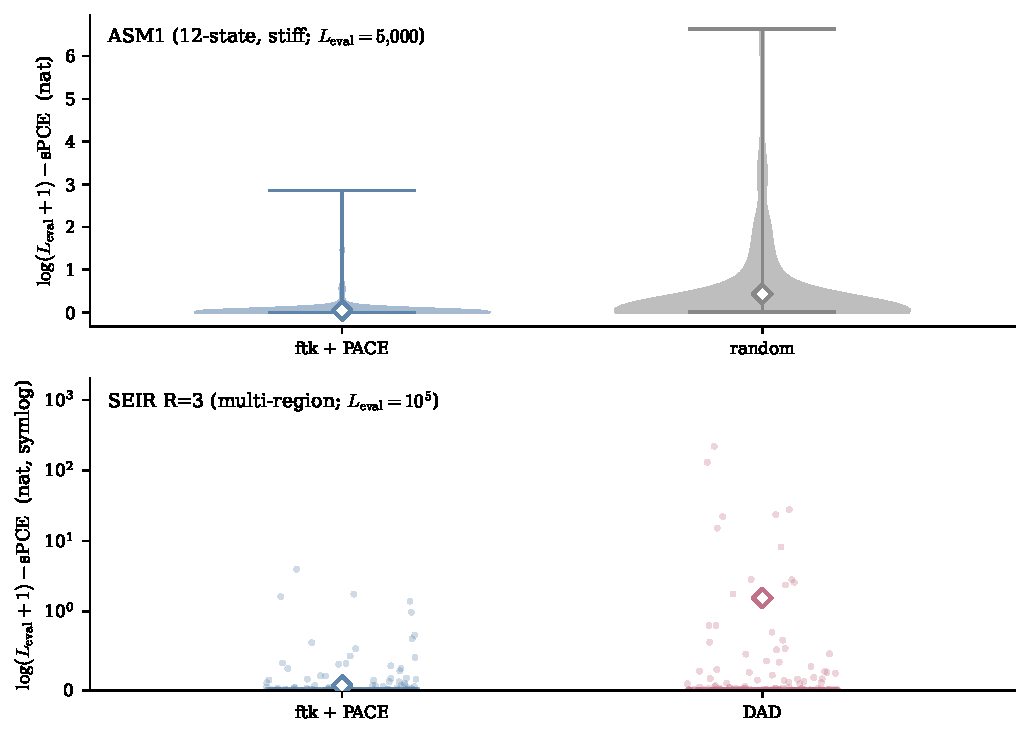
\includegraphics[width=0.6\linewidth]{figures/fig4b_anchors_violin.pdf}
  \caption[Rollout deficits on stiff anchors]{Per-rollout deficit from the evaluation
  ceiling on the stiff anchors, smaller is better. On ASM1 (top) PACE concentrates
  near zero deficit while random spreads below. On SEIR R=3 (bottom) the strip plot
  shows DAD's catastrophic tail, which PACE and random both avoid.}
  \label{fig:anchors}
\end{figure}

\section{Cross-system comparison: where saturation does not bite}
\label{sec:r-cross}

The lower block of Table~\ref{tab:results} covers systems with small escape
thresholds, where the policy trains without saturation and the comparison is
system-specific. PACE wins definitively on source location at $p{=}2$ ($+1.52$) and
$p{=}5$ ($+1.07$) and on the twenty-dimensional PK 8-compartment system ($+0.16$), and
ties DAD on both PK 1-compartment horizons, where the brackets overlap. The policy is
stronger on PI3K ($-0.14$) and on the highest-dimensional source-location task,
$p{=}8$ ($-0.34$). The crossover does not track parameter dimension: PK 8-comp at
$d_\theta=20$ favours PACE while PI3K at $d_\theta=6$ favours DAD. Nor does it track the
effective sample size, as Section~\ref{sec:r-perstep} shows. It tracks whether the
escape threshold exceeds the feasible training budget, which is the screening rule of
Section~\ref{sec:m-saturation}: wherever the threshold is large, PACE matches or beats
the policy. The losses on PI3K and source-location $p{=}8$ are genuine, confirmed by
tight brackets, and we examine in the ablation below whether they are due to the
estimator or the optimiser.

\section{Ablation study}
\label{sec:r-ablation}

The results combine two ingredients, the posterior-contrastive estimator and the
forward-only optimiser. We isolate them in turn. The controlled toy of
Section~\ref{sec:r-toy} already isolated the \emph{estimator}: holding the optimiser
fixed, replacing prior contrastives with posterior ones is what removes the saturation
bias. This section isolates the \emph{optimiser}.

Table~\ref{tab:ablation} compares PACE-grad (Algorithm~\ref{alg:grad}, gradient ascent
on the PACE score) against PACE-ftk (Algorithm~\ref{alg:ftk}, forward-only search) on
the seven systems where both were run. Both variants use the same one-time NPE proposal
and the same candidate budget, so the only difference is the optimiser. With the
proposal held fixed, the optimiser rarely helps and sometimes hurts. Gradient ascent
and forward-only search are statistically indistinguishable on both PK 1-comp horizons,
PK 8-comp, and source location $p{=}5$ ($p\ge0.13$). Gradient ascent helps in exactly
one place, source location $p{=}8$ ($6.27$ against $5.66$, $p=0.003$), where it
reverses the gap with DAD. It hurts on source location $p{=}2$, and most sharply on the
stiff PI3K system, where it loses $0.88$ nats and drops below DAD. On PI3K the adjoint
gradient is uninformative: gradient ascent improves on its random warm start by under
$0.2$ nats, so it reduces to a weaker candidate search than the cross-entropy method
already performs. This is the practical case for the forward-only default. The two
losses to DAD have different causes: on source location $p{=}8$ the optimiser is the
bottleneck and gradient ascent recovers the gap, whereas on PI3K the gradient is the
problem and forward-only search is the better choice.

\begin{table}[t]
\centering\small
\caption[Optimiser ablation]{Optimiser ablation. Both variants use the same one-time
NPE proposal and candidate budget; only the optimiser differs, forward-only
cross-entropy (ftk) versus gradient ascent on the PACE score (grad). Each cell is the
mean $\pm$ SEM over $n=300$ paired rollouts; lower bound ($\uparrow$) is sPCE, upper
bound ($\downarrow$) is sNMC. $\Delta_{\mathrm{sPCE}}$ is the paired grad${-}$ftk
difference $\pm$ SEM. Gradient ascent helps only where the simulator gradient is
reliable and hurts on stiff PI3K.}
\label{tab:ablation}
\begin{tabular}{lcccc c}
\toprule
& \multicolumn{2}{c}{PACE-grad} & \multicolumn{2}{c}{PACE-ftk} & \\
\cmidrule(lr){2-3}\cmidrule(lr){4-5}
System ($L_{\mathrm{eval}}$) & Lower bound\,$\uparrow$ & Upper bound\,$\downarrow$ & Lower bound\,$\uparrow$ & Upper bound\,$\downarrow$ & $\Delta_{\mathrm{sPCE}}$ ($p$) \\
\midrule
Src.\ loc.\ $p{=}2$ ($10^5$) & $8.79{\pm}0.12$ & $9.29{\pm}0.16$ & $9.12{\pm}0.11$ & $9.83{\pm}0.18$ & $-0.33{\pm}0.13$ ($9.4\mathrm{e}{-}3$) \\
Src.\ loc.\ $p{=}5$ ($10^5$) & $10.03{\pm}0.12$ & $12.86{\pm}0.32$ & $9.84{\pm}0.11$ & $11.89{\pm}0.27$ & $+0.19{\pm}0.15$ ($0.20$) \\
Src.\ loc.\ $p{=}8$ ($10^5$) & $6.27{\pm}0.17$ & $6.48{\pm}0.19$ & $5.66{\pm}0.17$ & $5.78{\pm}0.19$ & $+0.61{\pm}0.20$ ($3.1\mathrm{e}{-}3$) \\
PK 1-comp $T{=}3$ ($2$K) & $2.72{\pm}0.08$ & $2.74{\pm}0.08$ & $2.61{\pm}0.08$ & $2.63{\pm}0.09$ & $+0.11{\pm}0.09$ ($0.24$) \\
PK 1-comp $T{=}5$ ($2$K) & $3.23{\pm}0.08$ & $3.27{\pm}0.09$ & $3.25{\pm}0.09$ & $3.29{\pm}0.09$ & $-0.03{\pm}0.10$ ($0.78$) \\
PK 8-comp ($2$K)    & $2.16{\pm}0.07$ & $2.17{\pm}0.07$ & $2.26{\pm}0.07$ & $2.27{\pm}0.07$ & $-0.10{\pm}0.07$ ($0.13$) \\
PI3K $T{=}8$ ($10^5$) & $5.49{\pm}0.12$ & $5.55{\pm}0.13$ & $6.37{\pm}0.10$ & $6.45{\pm}0.12$ & $-0.88{\pm}0.07$ ($6.9\mathrm{e}{-}29$) \\
\bottomrule
\end{tabular}
\end{table}

\section{Per-step information and the effective sample size}
\label{sec:r-perstep}

Reading the rollouts step by step shows that performance follows the information
remaining in the posterior, not the effective sample size of the importance weights.
The per-step increment $\Delta S_t$ decays across steps for every method, which
reflects the contracting posterior, while the effective sample size collapses on a
separate schedule. Figure~\ref{fig:perstep} shows the two side by side on CES and SEIR
R=3. The cumulative per-step information of PACE exceeds random by $+0.5$ to $+5.6$
nats and exceeds DAD on the saturated systems; on CES the
totals are $+13.06$ for PACE against $+12.05$ for DAD and $+9.05$ for random, and on
SEIR R=3 they are $+14.83$ against $+7.46$ and $+14.15$.

\begin{figure}[t]
  \centering
  \begin{subfigure}[b]{0.49\linewidth}\centering
    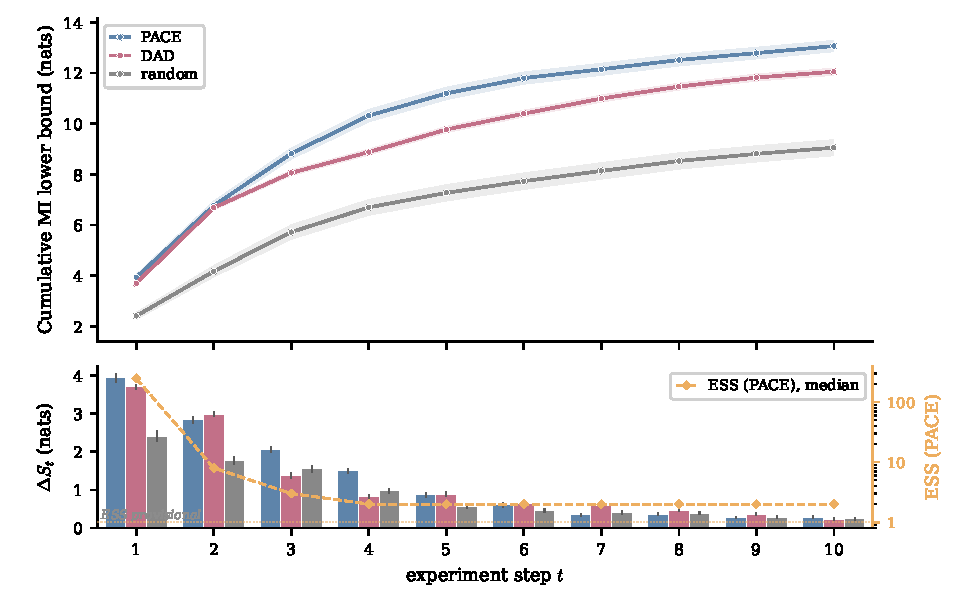
\includegraphics[width=\linewidth]{figures/fig_b7_perstep_eig_ess_CES.pdf}
    \caption{CES}\label{fig:perstep-ces}
  \end{subfigure}\hfill
  \begin{subfigure}[b]{0.49\linewidth}\centering
    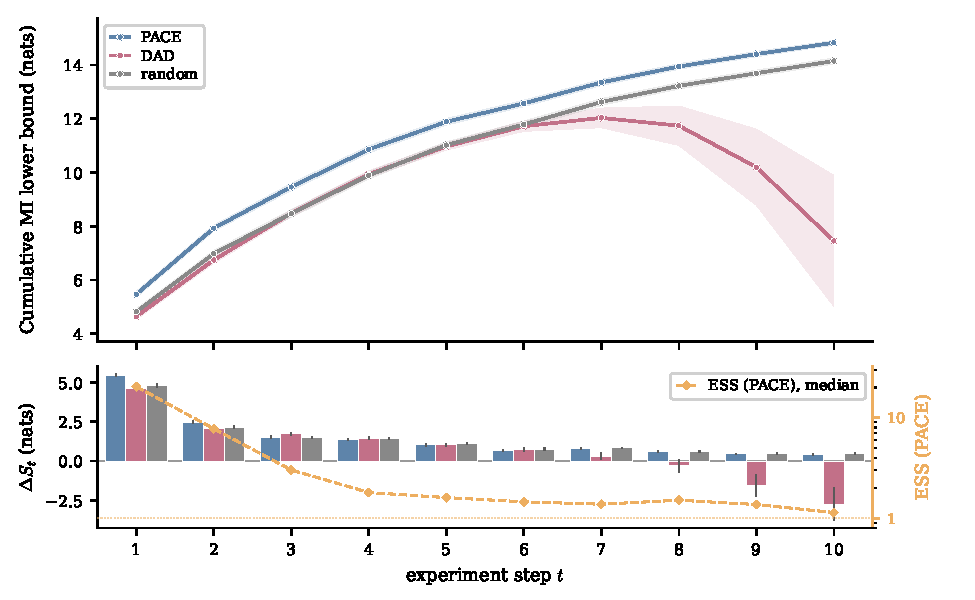
\includegraphics[width=\linewidth]{figures/fig_b7_perstep_eig_ess_SEIR_R_3.pdf}
    \caption{SEIR R=3}\label{fig:perstep-seir}
  \end{subfigure}
  \caption[Per-step information and effective sample size]{Per-step information and
  effective sample size on CES and SEIR R=3. Top of each panel: cumulative information
  for PACE, DAD, and random. Bottom: the per-step increment $\Delta S_t$ as bars, with
  the median PACE effective sample size overlaid (right axis, log scale). The increment
  decays with posterior concentration while the effective sample size collapses on its
  own schedule, yet PACE keeps its lead.}
  \label{fig:perstep}
\end{figure}

Three cases make the disconnect concrete. On SEIR R=3 the effective sample size falls
to one by the final step, yet the per-step gap over DAD grows from $+0.33$ nats in the
first third of the rollout to $+2.02$ nats in the last third, because DAD's late
designs collapse while PACE's stay informative. On CES the effective sample size pins at
about two from the second step onward, yet $70\%$ of PACE's total information is
acquired at an effective sample size of five or below, and the three steps at three or
below alone contribute $34\%$. The cleanest contrast is between PK 8-comp and PI3K. PK
8-comp is the only system that keeps a high effective sample size throughout, at least
$12\%$ of the particle count, yet PACE wins by only $+0.16$ nats; PI3K collapses to
about two like the others, yet also favours DAD by $-0.14$ nats. Neither retaining nor
losing the effective sample size fixes the sign of the gap. For this reason we do not
report a single cross-system correlation between the effective sample size and
performance: the sign of such a fit is not stable across summaries of the same
rollouts. The per-step view is the honest one, and it says performance is set by
whether the policy training signal is saturated, not by whether the importance weights
are degenerate. The full per-step and effective-sample-size tables are in
Appendix~\ref{app:supp}.

\section{Diagnostics: trusting the results under weight collapse}
\label{sec:r-diag}

A collapsing effective sample size looks alarming, so each diagnostic below rules out a
specific failure. The starting point is the identity of Eq.~\eqref{eq:widentity}: a
perfect proposal keeps the effective sample size at its maximum at any concentration,
so a collapse implies a small proposal mismatch amplified by concentration, not a
broken proposal. Four diagnostics confirm this.

First, the chosen design survives resampling. On ASM1, resampling the particle bank two
hundred times at several steps gives a median top-1 agreement of $45\%$ on which design
is selected, about twenty-three times the chance rate of one in fifty candidates. The
common-mode cancellation of Section~\ref{sec:m-cancellation} therefore preserves a
strong directional signal even when the weights have collapsed.

Second, the breakage is in the resampling, not the proposal. Table~\ref{tab:coverage}
separates the two. The coverage of the true parameter by the raw NPE samples, before
importance reweighting, stays between $76\%$ and $90\%$ through the final step on every
system. The coverage after importance resampling collapses, to $36\%$ on PI3K and
$32\%$ on CES at the last step, because resampling from degenerate weights shrinks the
credible set to almost a point. The proposal stays well calibrated; the collapse is a
resampling artifact.

\begin{table}[t]
\centering\small
\caption[Raw versus resampled coverage]{Per-step coverage of the true parameter at the
$90\%$ level, as a fraction of parameter dimensions. Raw is computed on NPE samples
before reweighting and tests the proposal directly; IS is computed after importance
resampling. ESS is the per-step median. Raw coverage stays high while IS coverage
collapses at late steps, isolating the resampling artifact.}
\label{tab:coverage}
\begin{tabular}{lccrcc}
\toprule
System & $d_\theta$ & step & ESS & raw @90\% & IS @90\% \\
\midrule
PK 8-comp & 20 & 1 & 233 & 90\% & 89\% \\
          &    & 5 & 125 & 90\% & 88\% \\
\cmidrule(l){1-6}
PI3K & 6 & 1 & 561 & 90\% & 90\% \\
     &   & 4 & 17 & 85\% & 80\% \\
     &   & 8 & 1.6 & 76\% & 36\% \\
\cmidrule(l){1-6}
CES & 4 & 1 & 8.6 & 88\% & 63\% \\
    &   & 5 & 2.6 & 85\% & 36\% \\
    &   & 10 & 1.7 & 84\% & 32\% \\
\cmidrule(l){1-6}
ASM1 & 12 & 1 & 77 & 90\% & 85\% \\
     &    & 3 & 5.7 & 87\% & 65\% \\
     &    & 5 & 2.7 & 87\% & 50\% \\
\bottomrule
\end{tabular}
\end{table}

Third, calibration is stable across steps. Simulation-based calibration on the raw NPE
samples gives a KS distance between $0.13$ and $0.18$ across systems, flat or improving
across steps, including on CES and ASM1 where the effective sample size falls below ten.
The same diagnostic on resampled samples degrades, which again points to a resampling
artifact rather than a proposal failure. The subtlety here is that calibration on
average, which is what simulation-based calibration tests, is not the same as
calibration at the specific histories where the effective sample size collapses. The
raw coverage in Table~\ref{tab:coverage}, measured at the deployment histories, is the
complementary conditional evidence; both are developed in Appendix~\ref{app:diagnostics}.

Fourth, there is no mode collapse. Gross mode collapse would show as Pareto shapes of
the weights diverging and raw coverage going to zero. Neither occurs: raw coverage
stays at or above $76\%$ and the calibration distances stay small. The method also
moves across more than a hundredfold in effective sample size across systems without
any threshold or mode switch, from the high-coverage multi-particle regime of PK 8-comp
to the single-particle regime of CES and ASM1, which confirms the smooth interpolation
of Section~\ref{sec:m-cancellation}. Together these diagnostics support the central
empirical claim of RQ3: PACE's design rankings are reliable even when its weights have
collapsed.

\section{Computational cost and the budget trade-off}
\label{sec:r-budget}

The cost transfer of Section~\ref{sec:m-pace} is the empirical counterpart of
contribution~2: PACE moves the per-step contrastive cost of policy training onto a
one-time inference pass plus a constant per-step search. This section collects the
budget evidence.

\paragraph{The two cost structures.} A policy trained on the sPCE objective pays, per
gradient step, $L_{\mathrm{train}}$ forward-plus-backward simulator solves, and on
saturated systems $L_{\mathrm{train}}$ must reach $L_{\mathrm{escape},50}$ before the
gradient carries signal (Section~\ref{sec:m-saturation}); the training cost scales as
$O(N_{\mathrm{iter}}\,L_{\mathrm{escape},50}\,T)$. PACE pays a one-time NPE training pass
plus, per step, $J(1+M(1+C)N_{\mathrm{cand}})$ forward-only solves
(Section~\ref{sec:m-forward}). The first grows exponentially with the information per
experiment; the second does not.

\paragraph{Measured costs.} Table~\ref{tab:walltime} reports the numbers. PACE's one-time
NPE training takes $3.6$ to $12.8$ minutes across the suite, and generating that training
data takes under a minute on the non-stiff systems and $5$ to $60$ minutes on the stiff
ones. At deployment PACE selects each design in under four seconds on eleven of twelve
systems, the exception being the stiff ASM1 model at $40.5$\,s. Policy training, by
contrast, ranges from about seven minutes on the simplest systems to sixteen hours on
Monod, is unstable on CES, and is infeasible on ASM1 and on SEIR R=3 at the budget needed
to escape saturation. A deployed policy then emits designs in milliseconds, faster than
PACE per step, but this latency gap is irrelevant for scientific experiments that take
minutes to weeks to run; the decisive comparison is the one-time training cost.

\paragraph{Budget versus quality.} Two results bound the trade-off. The cost-shift toy
(Figure~\ref{fig:toy}) sets the lower end: PACE reaches the true EIG once its NPE is
trained on only $500$ to $5000$ simulations, while the prior-contrastive estimator stays
pinned regardless of budget. The DAD L-sweep (Table~\ref{tab:dad-sweep}) sets the other
end: on SEIR R=3 the policy never escapes saturation across five orders of magnitude of
$L_{\mathrm{train}}$, so no feasible policy budget buys a usable design. Together they
make the cost transfer concrete: PACE's budget is bounded and paid once, whereas the
policy's required budget is unbounded on exactly the systems where design matters most.
% TODO(planned sweeps -- see PLANNED_EXPERIMENTS.md):
% A1 real-anchor N_NPE sweep (CES/SEIR) -> figure generalising the toy phase transition;
% A2 quality/cost vs particle count J; A3 quality vs CEM budget (N_cand, C).
% Drop figures/tables and a sentence here once the runs are complete.

        \chapter{Discussion}
\label{sec:discussion}

\section{When to use PACE}
\label{sec:d-when}

The results give a clear rule for when PACE is the right tool. It is preferred on
systems with broad priors, high information per experiment, and stiff or
non-differentiable dynamics, in low to moderate-dimensional continuous design
spaces. These are exactly the systems on which the prior-contrastive training
signal saturates, and the screening threshold $L_{\mathrm{escape},50}$ identifies
them before any policy is trained. On the saturated anchors, CES, SEIR R=3, and
ASM1, PACE matches or beats the policy, and on ASM1 it works where policy training
is infeasible.

Learned policies remain the better choice elsewhere. When the escape threshold is
small, the policy trains without saturation and its trajectory-level view can
capture design dependencies that a greedy per-step rule does not. This is what we
see on Monod, on PI3K, and on the highest-dimensional source location task. The
crossover is governed by saturation, not by parameter dimension and not by the
effective sample size, so the two methods are complementary rather than competing.

\section{Practical cost}
\label{sec:d-cost}

PACE shifts cost from a per-step policy-training budget to a one-time inference
pass plus a modest per-step search. Training the neural posterior estimator takes
between about $3.6$ and $12.8$ minutes once per system. At deployment, PACE selects
each design in under four seconds on eleven of the twelve systems, the exception
being the stiff ASM1 model at about forty seconds per step. By contrast, training a
policy ranges from a few minutes on the simplest systems to about sixteen hours on
Monod, and is unstable on CES and infeasible on ASM1 and on SEIR R=3 at the budget
needed to escape saturation. A deployed policy then produces designs in
milliseconds, which is faster than PACE per step, but this difference is irrelevant
for scientific experiments that take minutes to weeks to run. The full timing table
is in Appendix~\ref{app:walltime}.

\section{Limitations}
\label{sec:d-limits}

Several limitations qualify the conclusions. The forward-only search does not scale
to high-dimensional or combinatorial design spaces, where a learned policy is
stronger; the source location result at $p{=}8$ is the clearest case, and the
ablation shows the optimiser rather than the estimator is the bottleneck there.
Under a collapsed effective sample size, PACE produces reliable design rankings but
not calibrated EIG values, so it should be read as an acquisition criterion rather
than an absolute information estimate. The method assumes the neural posterior
estimator does not collapse onto the wrong mode; this is benign for the unimodal
posteriors of well-observed ODE systems but is a genuine risk under strong
multimodality, and it must be checked with the diagnostics of
Section~\ref{sec:r-diag}. The Gaussian-linearised threshold $\Lambda$ is a
qualitative guide, not a quantitative predictor, on stiff systems. Finally, the
study evaluates greedy design and a fixed myopic horizon; non-myopic extensions are
left open.

On reproducibility and validity, all main comparisons use $n=300$ paired rollouts
with paired tests and report both bounds on the EIG, so the orderings marked
definitive cannot be reversed by estimation slack. Earlier small-sample estimates
were replaced by these larger paired runs.

\section{Broader impact}
\label{sec:d-impact}

More efficient experimental design reduces the number of experiments needed to
learn a system, which lowers the cost, time, and material or animal use of
scientific work in areas such as pharmacokinetics, wastewater treatment, and
bioprocessing. The same machinery applies to epidemic intervention design, where
recommendations can affect public health policy and should be used with appropriate
caution and human oversight. PACE also makes its own uncertainty visible through the
diagnostics it reports, which supports honest use under model misspecification
rather than overconfident automation.

        \chapter{Conclusion}
\label{sec:conclusion}

This thesis set out to make sequential Bayesian experimental design feasible and
effective on stiff, broad-prior dynamical systems where amortized policy methods
fail. It answered the main question in the affirmative, through four results linked
by a single quantity, the likelihood ratio and its prior average $e^{-\Lambda}$.

In answer to RQ1, the prior-contrastive sPCE objective that policy methods are
trained on saturates at $\log(L+1)$ nats, its gradient vanishes at the same rate,
and the contrastive budget needed to escape grows as $e^{\Lambda}$. The failure can
be quantified before training through the escape threshold, which ranges from below
ten to above a million across the suite. In answer to RQ2, drawing contrastives
from a posterior estimator trained once by simulation-based inference removes the
saturation, because the likelihood factor in the importance weight cancels the
divergence that defeated prior contrastives; the cost does not vanish but moves, as
the same posterior concentration reappears in the decline of the effective sample
size. In answer to RQ3, design selection stays valid under that decline, because
the diverging weight scale enters only design-independent terms and cancels in the
ranking, and the criterion approaches a Fisher-information rule in the limit. In
answer to RQ4, PACE matches or beats the policy on every system where the policy
training signal has saturated, including a stiff wastewater model on which the
policy cannot be trained, while learned policies remain stronger on low-information,
high-dimensional designs; the crossover is predicted by the saturation threshold,
not the effective sample size.

The contribution is therefore both a diagnosis and a method. The diagnosis explains
why a widely used training signal fails on an important class of systems, and gives
a cheap test for when it will. The method escapes that failure with a forward-only
estimator that needs neither a trained policy nor gradients through the simulator,
and it remains valid in the regime that makes the problem hard.

The conclusions are qualified by the limitations discussed above. The forward-only
search does not scale to high-dimensional combinatorial designs, PACE returns
reliable rankings rather than calibrated information values under collapsed weights,
and the method assumes a posterior estimator that does not collapse onto the wrong
mode. Future work that addresses these would combine the posterior-contrastive score
with a learned proposal policy to recover scalability, use observation-conditional
inner proposals to keep the effective sample size higher, extend the design rule
beyond a greedy horizon, and test the method on the timed-input biochemical systems
that motivated it.


\bibliographystyle{plainnat}
\bibliography{bibliographies/references}

% \newpage
\appendix
        % Appendix. The main text is self-contained; this is supporting detail.

\chapter{Standard background derivations}
\label{app:background}

This appendix records the established results used in Section~\ref{sec:m-prelim}.
They are not contributions of this thesis; they are collected here so the main text
can state them briefly.

The trajectory information bound (Eq.~\eqref{eq:traj-mi}) is derived in the main text
(Section~\ref{sec:m-policy}); we record only the contrastive bounding properties and
the per-step chain rule here.

\section{Bounding properties of the contrastive estimators}
\label{app:bounds}

Recall $\mathrm{sPCE}_L$ from Eq.~\eqref{eq:spce} and $\mathrm{sNMC}_L$, which uses
the same numerator but divides the denominator sum by $L$ over the contrastives
$\theta_{1:L}$ only.

\paragraph{sPCE is a lower bound, capped at $\log(L+1)$.}
The denominator of sPCE is an average over $L+1$ likelihoods that estimates the
same marginal $p(y_t\mid\xi_t,h_{t-1})$, but it includes the data-generating
$\theta_0$, whose likelihood is systematically large for the $y_t$ it produced.
This biases the denominator up and the ratio down, so
$\mathbb{E}[\mathrm{sPCE}_L]\le I_{h_{t-1}}(\xi_t)$. Equivalently, sPCE is a
classification bound: among the $L+1$ exchangeable draws, identifying which
generated $y_t$ has success probability at most one, so
$\mathbb{E}[\mathrm{sPCE}_L]=\log(L+1)-H(\text{index}\mid\theta_{0:L},y_t)\le\log(L+1)$.

\paragraph{sNMC is an upper bound.}
The denominator $\frac1L\sum_{\ell=1}^L p(y_t\mid\theta_\ell,\xi_t)$ is an unbiased
estimate of the marginal. By Jensen's inequality the expected log of an unbiased
estimate underestimates the log of the mean, so the log-marginal is underestimated
and the ratio overestimated, giving $\mathbb{E}[\mathrm{sNMC}_L]\ge I_{h_{t-1}}(\xi_t)$.

Both biases are $O(1/L)$, so $[\mathrm{sPCE}_L,\mathrm{sNMC}_L]$ brackets the true
EIG and tightens as $L\to\infty$.

\section{Per-step chain rule}
\label{app:chain}

Let $S_t$ be the sPCE evaluated on the length-$t$ prefix and $S_0=0$. The per-step
increment $\Delta S_t=S_t-S_{t-1}$ telescopes, $\sum_{t=1}^{T}\Delta S_t=S_T$,
recovering the trajectory bound. Each $\Delta S_t$ weights the contrastive
denominator by the running posterior, so it measures the information acquired at
step $t$ within the operative posterior rather than from a fresh prior estimate.

\chapter{Linearised EIG and the escape threshold}
\label{app:lindley}

\section{The linearised information gain equals $\Lambda$}
The main text calls $\Lambda$ the Gaussian-linearised information gain; we justify the
name. For a Gaussian prior $p(\theta)=\mathcal N(\mu_0,\Sigma_0)$ and a linear-Gaussian
observation $y=\mu_0+J(\theta-\theta_0)+\varepsilon$ with $\varepsilon\sim\mathcal N(0,R)$,
the posterior is Gaussian with covariance $\Sigma_{\mathrm{post}}=(\Sigma_0^{-1}+F)^{-1}$,
$F=J^\top R^{-1}J$, which does not depend on the realised $y$. The information gain is the
drop in differential entropy,
\begin{align}
\mathrm{EIG}(\xi)
&= H[p(\theta)]-\mathbb{E}_y\,H[p(\theta\mid y,\xi)]
= \tfrac12\log\!\big((2\pi e)^d\det\Sigma_0\big)-\tfrac12\log\!\big((2\pi e)^d\det\Sigma_{\mathrm{post}}\big)\nonumber\\
&= \tfrac12\log\frac{\det\Sigma_0}{\det\Sigma_{\mathrm{post}}}
= \tfrac12\log\det\!\big(\Sigma_0(\Sigma_0^{-1}+F)\big)
= \tfrac12\log\det(I+\Sigma_0 F)
= \tfrac12\sum_i\log(1+\lambda_i)=\Lambda. \label{eq:eig-lambda}
\end{align}
So $\Lambda$ is exactly the EIG of the linearised experiment (equivalently the Bayesian
D-optimal value). For nonlinear models the same expression is the leading term of the
entropy-based EIG under a Gauss--Newton (Laplace) approximation, with $\Sigma_{\mathrm{post}}$
evaluated at the posterior mode. Combined with the escape result below, this gives the
headline relation $L_{\mathrm{escape}}\sim e^{\Lambda}=e^{\mathrm{EIG}}$: the contrastive
budget needed to escape saturation grows as the exponential of the experiment's
information.

\paragraph{Interpretation.} Each $\lambda_i$ is a per-axis signal-to-noise ratio. It is
an eigenvalue of the prior-scaled Fisher information $\Sigma_0^{1/2}F\Sigma_0^{1/2}$,
comparing how much the experiment informs direction $i$ (through $F$) against the prior
uncertainty there (through $\Sigma_0$). A well-identified direction has $\lambda_i\gg1$
and contributes $\tfrac12\log(1+\lambda_i)\approx\tfrac12\log\lambda_i$ nats; a
barely-informed direction has $\lambda_i\ll1$ and contributes almost nothing. $\Lambda$
is the sum of these per-axis contributions, and $e^{\Lambda}=\prod_i(1+\lambda_i)^{1/2}$
is the factor by which the posterior volume shrinks below the prior, which is exactly
the contrastive budget needed to escape saturation.

\section{The expected importance weight and the escape threshold}
We derive in full the scaling $\mathbb{E}[r_\ell]\sim e^{-\Lambda}$ stated in
Eq.~\eqref{eq:escape-scale}, via the marginal-likelihood route. Take a Gaussian prior
$p(\theta)=\mathcal N(\mu_0,\Sigma_0)$ and observation $y=\mu(\theta,\xi)+\varepsilon$
with $\varepsilon\sim\mathcal N(0,R)$. The Fisher information is $F=J^\top R^{-1}J$
with $J=\partial\mu/\partial\theta|_{\theta_0}$, and the posterior precision is
$\Sigma_{\mathrm{post}}^{-1}=\Sigma_0^{-1}+F$.

\paragraph{Step 1: Laplace approximation to the marginal likelihood.}
Expand the log-likelihood to second order about $\theta_0$,
\[
\log p(y\mid\theta,\xi) \approx \log p(y\mid\theta_0,\xi) + (\theta-\theta_0)^\top s - \tfrac12(\theta-\theta_0)^\top F(\theta-\theta_0),
\]
where $s=\nabla_\theta\log p(y\mid\theta,\xi)|_{\theta_0}$ is the score and the
curvature is the observed information $H=-\nabla_\theta^2\log p(y\mid\theta,\xi)|_{\theta_0}$;
under Gaussian noise $H=J^\top R^{-1}J=F$ exactly, and for general likelihoods
$\mathbb{E}_y[H]=F$, so we use $F$ throughout. Adding the Gaussian log-prior and
completing the square,
\[
\log\bigl[p(y\mid\theta,\xi)\,p(\theta)\bigr] \approx \log\bigl[p(y\mid\theta_0,\xi)\,p(\theta_0)\bigr] + \tfrac12 g^\top\Sigma_{\mathrm{post}}\,g - \tfrac12(\theta-\hat\theta)^\top\Sigma_{\mathrm{post}}^{-1}(\theta-\hat\theta),
\]
where $g=s-\Sigma_0^{-1}(\theta_0-\mu_0)$ is the log-posterior gradient at $\theta_0$
and $\hat\theta=\theta_0+\Sigma_{\mathrm{post}}\,g$ is the posterior mode. The
unnormalised posterior is thus approximately Gaussian with covariance
$\Sigma_{\mathrm{post}}$; integrating the Gaussian kernel
($\int = (2\pi)^{d/2}\det(\Sigma_{\mathrm{post}})^{1/2}$),
\[
p(y\mid\xi) \approx p(y\mid\theta_0,\xi)\,p(\theta_0)\,e^{\frac12 g^\top\Sigma_{\mathrm{post}}\,g}\,(2\pi)^{d/2}\det(\Sigma_{\mathrm{post}})^{1/2}.
\]

\paragraph{Step 2: Expected importance weight.}
From Eq.~\eqref{eq:Er}, $\mathbb{E}[r_\ell]=\int p(y\mid\theta,\xi)\,p(\theta)\,\ud\theta\,/\,p(y\mid\theta_0,\xi)$.
Substituting the Laplace marginal and the Gaussian prior density
$p(\theta_0)=(2\pi)^{-d/2}\det(\Sigma_0)^{-1/2}\exp(-\tfrac12(\theta_0-\mu_0)^\top\Sigma_0^{-1}(\theta_0-\mu_0))$,
\[
\mathbb{E}[r_\ell] \approx \underbrace{\frac{\det(\Sigma_{\mathrm{post}})^{1/2}}{\det(\Sigma_0)^{1/2}}}_{\text{(1) volume ratio}} \cdot \underbrace{\exp\!\Bigl(-\tfrac12(\theta_0-\mu_0)^\top\Sigma_0^{-1}(\theta_0-\mu_0)\Bigr)}_{\text{(2) prior centering}} \cdot \underbrace{e^{\frac12 g^\top\Sigma_{\mathrm{post}}\,g}}_{\text{(3) mode shift}}.
\]
Factor (1) is the exponentially small volume ratio that drives saturation. Factor (2)
involves a Mahalanobis distance that is $\chi^2_d$ with mean $d$, so it is
$e^{-\Theta(d)}$ (at the mean exponent, $e^{-d/2}$; in exact expectation
$\mathbb{E}[e^{-\frac12\chi^2_d}]=2^{-d/2}$). Factor (3) is $\ge1$ with exponent
$O(d)$. Factors (2) and (3) push in opposite directions, contribute $O(d)$ to the
exponent, and do not affect the exponential scaling in $\Lambda$. Retaining the
leading volume ratio,
\[
\mathbb{E}[r_\ell]\sim\frac{\det(\Sigma_{\mathrm{post}})^{1/2}}{\det(\Sigma_0)^{1/2}}=\frac{1}{\det(I+\Sigma_0 F)^{1/2}}=\prod_i(1+\lambda_i)^{-1/2}=e^{-\Lambda}.
\]

\paragraph{Step 3: Eigenvalue identity.}
$\Sigma_0 F$ is similar to the symmetric positive semidefinite matrix
$M:=\Sigma_0^{1/2}F\Sigma_0^{1/2}$ through $P=\Sigma_0^{1/2}$,
\[
P\,M\,P^{-1}=\Sigma_0^{1/2}\bigl(\Sigma_0^{1/2}F\Sigma_0^{1/2}\bigr)\Sigma_0^{-1/2}=\Sigma_0 F .
\]
Similar matrices share eigenvalues, and $M$ is symmetric PSD, since for any $v$,
$v^\top M v=(\Sigma_0^{1/2}v)^\top F(\Sigma_0^{1/2}v)\ge0$; its eigenvalues
$\lambda_i\ge0$ are therefore real. Hence
\[
\det(I+\Sigma_0 F)=\det(I+M)=\prod_i(1+\lambda_i),
\qquad \Lambda=\tfrac12\sum_i\log(1+\lambda_i).
\]

\paragraph{Step 4: Escape threshold.}
The expected contrastive sum is $\mathbb{E}[S]=L\,e^{-\Lambda}$. By Markov's
inequality $\Pr(S\ge1)\le\mathbb{E}[S]=L\,e^{-\Lambda}$, so saturation persists while
$\mathbb{E}[S]\ll1$, i.e.\ $L\ll e^{\Lambda}$, and escape requires
$L\gtrsim e^{\Lambda}$. $\square$

\paragraph{Correction factors.}
The combined effect of factors (2) and (3) shifts $L_{\mathrm{escape},50}$ by a
multiplicative factor $\sim e^{O(d)}$, large in absolute terms for $d=12$ (ASM1) but
subexponential relative to $e^{\Lambda}$ when $\Lambda\gg d$. Table~\ref{tab:escape-full}
reports the full twelve-system measurements; the structural mechanisms that push the
\emph{empirical} threshold beyond this Laplace prediction are derived in the main text
(Section~\ref{sec:m-mechanisms}).

\begin{table}[h]
\centering\small
\caption[Full saturation thresholds]{Empirical escape thresholds at random designs,
sorted ascending, with the Laplace reference $e^\Lambda$ where available. Stiff and
Hill-kinetic systems exceed $e^\Lambda$ by one to three orders of magnitude.}
\label{tab:escape-full}
\begin{tabular}{lccrrl}
\toprule
System & $d_\theta$ & $d_\xi$ & $\Lambda$ & $e^{\Lambda}$ & $L_{\mathrm{escape},50}$ \\
\midrule
PK 8-comp & 20 & 1 & $0.05$ & $1.1$ & ${\le}10$ \\
PK 1-comp & 4 & 1 & $1.02$ & $2.8$ & ${\sim}10$ \\
PI3K      & 6 & 2 & $1.49$ & $4.4$ & ${\le}10$ \\
Monod     & 2 & 1 & $4.30$ & $74$ & ${\sim}30$ \\
CES       & 4 & 6 & -- & -- & ${\sim}10^4$ (static) \\
Goodwin   & 5 & 1 & $4.40$ & $81$ & ${\sim}10^4$ \\
ASM1      & 12 & 2 & -- & -- & ${\sim}10^4$ (stiff) \\
SEIR R=3  & 9 & 9 & $8.64$ & $5{,}648$ & ${>}10^6$ \\
SEIR R=8  & 14 & 24 & $21.26$ & $1.7{\times}10^9$ & ${>}10^6$ \\
\bottomrule
\end{tabular}
\end{table}

\chapter{PACE: consistency, decomposition, and the Fisher limit}
\label{app:pace}

\section{Consistency}
Theorem~\ref{thm:consistency} is the standard two-stage self-normalized importance
sampling result. Support inclusion makes the weighted averages in the numerator and
denominator of Eq.~\eqref{eq:pace} converge almost surely to the corresponding
posterior expectations; finite chi-square divergence gives the $O(1/J)$ bias rate
through the SNIS central limit theorem. With a perfect proposal the weights are the
constant of Eq.~\eqref{eq:widentity} and the estimator is exact in the weights.

\section{Finite variance and the likelihood-factor cancellation}
\label{app:chi2}
The $O(1/J)$ rate in Theorem~\ref{thm:consistency} requires the chi-square divergence
$\chi^2(p(\cdot\mid h)\,\|\,q_\phi(\cdot\mid h))=\mathbb{E}_{q_\phi}\!\big[(p(\theta\mid h)/q_\phi(\theta\mid h))^2\big]-1$
to be finite, which holds for any NPE that covers the posterior. It is worth seeing why
PACE's weight has this property when the naive alternative does not. Estimating the
per-step gain by drawing contrastives from $q_\phi$ but \emph{targeting the prior
marginal}, as a prior-contrastive denominator does, would weight each draw by
$p(\theta_\ell)/q_\phi(\theta_\ell\mid h)$, whose divergence is
\begin{equation}
\label{eq:chi2-prior}
\chi^2\!\big(p(\theta)\,\big\|\,q_\phi(\cdot\mid h)\big)=\int\frac{p(\theta)^2}{q_\phi(\theta\mid h)}\,\ud\theta-1 .
\end{equation}
Since $q_\phi(\cdot\mid h)$ approximates the concentrated posterior, it has negligible
mass in the prior-dominated tails where $p(\theta)$ does not vanish, so the integrand
$p(\theta)^2/q_\phi(\theta\mid h)$ diverges and this $\chi^2$ is unbounded. PACE's weight
is instead
\[
w_j=\frac{p(\theta_j)\,p(h\mid\theta_j)}{q_\phi(\theta_j\mid h)}\;\propto\;\frac{p(\theta_j\mid h)}{q_\phi(\theta_j\mid h)} ,
\]
where the likelihood factor $p(h\mid\theta_j)$ is small exactly in those prior tails and
cancels the divergence, leaving the posterior-to-proposal ratio whose $\chi^2$ is finite
for a covering NPE. This cancellation is what makes the cost transfer of
Section~\ref{sec:m-costtransfer} work: the same likelihood factor that retargets the
estimator from the prior to the posterior is what keeps its variance finite.

\section{Decomposition}
Substituting $\tilde w_k=w_k/W$ with $W=\sum_k w_k$ into Eq.~\eqref{eq:pace} and
factoring $p(y_{t,j}\mid\theta_j,\xi_t)$ out of the inner sum using
$r_{k\leftarrow j}=p(y_{t,j}\mid\theta_k,\xi_t)/p(y_{t,j}\mid\theta_j,\xi_t)$ gives,
for the $j$-th term, $\log W-\log w_j-\log[1+\Psi_j(\xi_t)]$ with
$\Psi_j(\xi_t)=\sum_{k\ne j}(w_k/w_j)r_{k\leftarrow j}$. Taking the weighted sum and
using $\sum_j\tilde w_j\log w_j=-H(\tilde w)+\log W$ yields Eq.~\eqref{eq:decomp},
$\hat I^{\mathrm{PACE}}=H(\tilde w)-\bar\Phi(\xi_t)$. The collapsed-weight limit of
Eq.~\eqref{eq:lr-limit} follows as in Section~\ref{sec:m-decomp}.

\section{The Fisher limit}
We expand the collapsed-weight criterion of Section~\ref{sec:m-collapse}. When a single
competitor $\theta_{k^\ast}=\arg\max_{k\ne\mathrm{dom}}w_k$ dominates the remaining
non-dominant particles, the design-dependent term reduces to one summand,
\begin{equation}
\label{eq:pairwise}
\bar\Phi(\xi_t)\approx\frac{w_{k^\ast}}{w_{\mathrm{dom}}}\,r_{k^\ast\leftarrow\mathrm{dom}}(\xi_t)
=\frac{w_{k^\ast}}{w_{\mathrm{dom}}}\,\frac{p(y_{t,\mathrm{dom}}\mid\theta_{k^\ast},\xi_t)}{p(y_{t,\mathrm{dom}}\mid\theta_{\mathrm{dom}},\xi_t)} .
\end{equation}
The prefactor $w_{k^\ast}/w_{\mathrm{dom}}$ is constant in $\xi_t$, so minimising
$\bar\Phi$ is maximising the pairwise log likelihood-ratio
$\log[p(y_{t,\mathrm{dom}}\mid\theta_{\mathrm{dom}},\xi_t)/p(y_{t,\mathrm{dom}}\mid\theta_{k^\ast},\xi_t)]$.
Its expectation over $y_{t,\mathrm{dom}}\sim p(y_t\mid\theta_{\mathrm{dom}},\xi_t)$ is the
Kullback-Leibler divergence
\[
\mathbb{E}_{y_{t,\mathrm{dom}}}\!\left[\log\frac{p(y_{t,\mathrm{dom}}\mid\theta_{\mathrm{dom}},\xi_t)}{p(y_{t,\mathrm{dom}}\mid\theta_{k^\ast},\xi_t)}\right]
= D_{\mathrm{KL}}\!\big(p(y_t\mid\theta_{\mathrm{dom}},\xi_t)\,\|\,p(y_t\mid\theta_{k^\ast},\xi_t)\big) .
\]
For Gaussian likelihoods with a linearised forward map
$\mu(\theta,\xi_t)\approx\mu(\theta_{\mathrm{dom}},\xi_t)+J_{\xi_t}(\theta-\theta_{\mathrm{dom}})$,
this reduces to
$\tfrac12(\theta_{\mathrm{dom}}-\theta_{k^\ast})^\top F(\xi_t)(\theta_{\mathrm{dom}}-\theta_{k^\ast})$
with $F(\xi_t)=J_{\xi_t}^\top R^{-1}J_{\xi_t}$, and treating $\theta_{k^\ast}$ as a
posterior draw with covariance $\Sigma_{\mathrm{post}}$ gives the expected criterion
$\tfrac12\,\mathrm{tr}(F(\xi_t)\Sigma_{\mathrm{post}})$, a trace approximation to the
Gaussian-linearised (D-optimal) EIG.

This KL connection holds only for the pairwise case. The general weighted-sum criterion
of Eq.~\eqref{eq:lr-limit} is a sum of likelihood \emph{ratios}, not log-ratios, and
their expectations are constant in the design,
$\mathbb{E}_{y_{t,\mathrm{dom}}}[r_{k\leftarrow\mathrm{dom}}]=\int p(y\mid\theta_k,\xi_t)\,\ud y=1$;
there it is the realised $y_{t,\mathrm{dom}}$, not its expectation, that carries the
design signal.

\section{The dominant particle, and why standard IS fixes do not help}
\label{app:domparticle}
Under a collapsed weight set the dominant particle $\theta_{\mathrm{dom}}$ is the
posterior draw that the NPE most \emph{undercovers}: its self-normalised weight
$\tilde w_j\propto p(\theta_j\mid h)/q_\phi(\theta_j\mid h)$ is largest where the proposal
places too little mass relative to the true posterior, typically a posterior-tail
sample. This is why design selection keeps a signal even as $\mathrm{ESS}\to1$: the
criterion of Eq.~\eqref{eq:lr-limit} discriminates this tail representative from the
bulk rather than collapsing onto the posterior mean.

Two natural alternatives are worse. Dropping the importance weights and scoring with the
raw NPE particles fails because, once the posterior is tight, all $J$ particles cluster
near $\theta_{\mathrm{dom}}$, every ratio $r_{k\leftarrow j}\approx1$, and the score is
flat across designs; the reweighting is what keeps a discriminative contrastive in the
bank. Standard remedies for heavy-tailed importance weights also do not apply here.
Pareto-smoothed importance sampling~\citep{vehtari2024pareto} assumes a finite-variance
tail (Pareto $\hat k<0.7$), whereas here $\hat k$ is large by construction; truncating
the weights trades the (cancelling) variance for a bias that dominates at
$\mathrm{ESS}/J\sim10^{-3}$; and defensive mixtures that fold the prior back into the
proposal reintroduce exactly the prior-contrastive cost $L_{\mathrm{escape}}$ that PACE
removes. PACE instead accepts the collapse and relies on common-mode cancellation, which
requires only that the weights are shared across candidate designs.

\chapter{Supplementary tables}
\label{app:supp}

Table~\ref{tab:ess-full} reports the deployment-time effective sample size across
steps. It declines on every system but does not track the performance gap: see
Section~\ref{sec:r-perstep}. For the per-step increments $\Delta S_t$, the
cumulative $\sum_t\Delta S_t$ for PACE is $+13.06$ on CES (DAD $+12.05$, random
$+9.05$) and $+14.83$ on SEIR R=3 (DAD $+7.46$, random $+14.15$), and exceeds random
on every system in the suite.

\begin{table}[h]
\centering\footnotesize
\caption[Effective sample size trajectories]{Median per-step effective sample size from
production rollouts ($J=1000$; reported at $J=1000$ for ASM1 for comparability). The
decline is monotone from the first step and universal; all eight systems reach
$\mathrm{ESS}\le3$ by the final step, yet the decline does not track the performance
gap (Section~\ref{sec:r-perstep}). Only PK 8-comp (omitted, $\mathrm{ESS}/J\approx12$
to $23\%$ throughout) retains a high effective sample size.}
\label{tab:ess-full}
\begin{tabular}{l c >{\raggedright\arraybackslash}p{8.2cm} l}
\toprule
System & $T$ & ESS per step (median) & $\Delta_{\mathrm{sPCE}}$ \\
\midrule
Monod & 14 & 841, 612, 330, 125, 68, 39, 36, 18, 17, 10, 5, 3, 2, 1 & $-0.66$ vs DAD \\
CES & 10 & 9, 2, 2, 2, 3, 2, 2, 3, 2, 2 & $+0.93$ vs DAD \\
Src.\ loc.\ $p{=}2$ & 10 & 40, 29, 15, 12, 6, 3, 2, 2, 2, 1 & $+1.52$ vs DAD \\
Src.\ loc.\ $p{=}5$ & 30 & 93, 75, 39, 37, 32, 29, 21, 18, 13, 11, 8, 7, 6, 5, 6, 5, 4, 4, 4, 3, 3, 3, 3, 3, 3, 2, 2, 2, 2, 2 & $+1.07$ vs DAD \\
PI3K & 8 & 561, 285, 87, 17, 8, 3, 3, 2 & $-0.14$ vs DAD \\
SEIR R=3 & 10 & 20, 8, 3, 2, 2, 1, 1, 2, 1, 1 & $+7.31$ vs DAD \\
ASM1 & 5 & 77, 16, 6, 3, 3 & $+0.89$ vs rand. \\
Goodwin & 10 & 169, 81, 37, 23, 12, 8, 6, 5, 6, 2 & $-0.48$ vs rand. \\
\bottomrule
\end{tabular}
\end{table}

% AUTO-GENERATED by scripts/_gen_perstep_table.py — do not edit by hand.
% Re-run after adding systems to outputs/_perstep_compiled/.

\section{Per-step EIG contribution under ESS collapse}
\label{sec:perstep-dS}

Table~\ref{tab:ess-full} shows the IS-weight ESS collapsing across BED steps;
Table~\ref{tab:perstep-dS} shows the per-step \emph{information} still
contributed despite that collapse. We report per-step increments
$\Delta S_t = S_t - S_{t-1}$, where $S_t$ is the sPCE bound
[Eq.~\eqref{eq:spce}] evaluated on the length-$t$ prefix $\hist_t$ (with $S_0=0$
and $S_T=\mathrm{sPCE}_T$). By the chain rule of mutual information these
telescope, $\sum_{t=1}^{T}\Delta S_t = S_T$, approximately recovering the trajectory bound
(last column of Table~\ref{tab:perstep-dS}); each $\Delta S_t$ estimates the
conditional EIG $I(\theta;y_t\mid\hist_{t-1})$ [Eq.~\eqref{eq:step-eig}] at the
realized $y_t$. Crucially, $S_t$ weights the contrastive denominator by the
running posterior $w^{(t-1)}_\ell\propto p(\hist_{t-1}\mid\theta_\ell)$, the same
importance weights of \S\ref{sec:m-costtransfer} whose ESS collapses as the
posterior contracts, so $\Delta S_t$ measures per-step information \emph{within}
the degenerate-weight regime rather than from a fresh prior-contrastive
estimate.\footnote{This conditional increment differs from the marginal
per-step sPCE (uniform contrastives, targeting $I(\theta;y_t)$), whose sum
overcounts $\mathrm{sPCE}_T$ by the total correlation among observations and is
blind to the collapse. As a numerical check, $\sum_t\Delta S_t$ matches the
trajectory sPCE of Table~\ref{tab:results} to within MC error on cells with
matching evaluation protocol.}

\textbf{Findings.}
\emph{(i) Per-step EIG decay tracks posterior concentration, not ESS.}
$\Delta S_t$ decays across steps for every method, but this reflects the
information remaining in a contracting posterior, \emph{not} the IS-weight ESS
collapse of Table~\ref{tab:ess-full}, from which it is empirically decoupled.
On CES the ESS pins at ${\approx}2$ from step~2 onward, yet $70\%$ of PACE's total
information is still acquired at $\mathrm{ESS}\leq 5$ (steps~3--5 alone, at
$\mathrm{ESS}\leq 3$, contribute $34\%$); on source-location $p{=}2$ the
PACE$-$random per-step gap holds at $\approx{+}0.3$ nat through the late steps
(8--10) where $\mathrm{ESS}\leq 5$. SEIR~R=3 is the extreme case: its ESS
collapses to $1$ by step~$10$ (Table~\ref{tab:ess-full}), yet the per-step
PACE$-$DAD gap \emph{grows} from $+0.33$ nat (first third) to $+2.02$ nat
(last third), as DAD's late designs collapse (Table~\ref{tab:dad-sweep})
while PACE's stay informative. Conversely, PK 8-comp keeps
$\mathrm{ESS}/J\geq 12\%$ throughout (PI3K, once thought similar, in fact
collapses to $\mathrm{ESS}\approx 2$ under the deployed random NPE), yet its
$\Delta S_t$ decays just as steeply. Per-step design quality follows the information remaining, not the
ESS: the per-step, mechanistic counterpart of the aggregate result that ESS
does not predict performance (\S\ref{sec:r-perstep}).
\emph{(ii) The cumulative advantage holds throughout.} PACE's
$\Sigma_t\Delta S_t$ exceeds random by $+0.5$ to $+5.6$
nat on each system in this table, and exceeds DAD on CES, SEIR~R=3, source-location $p{=}2$ and $p{=}5$,
PK~8-comp, and PK~1-comp $T{=}5$; it ties PK~1-comp $T{=}3$ and trails DAD on
Monod, PI3K, and source-location $p{=}8$ (consistent with
Table~\ref{tab:results}). The few late steps
at which PACE dips below random do so by small margins (at most $0.10$ nat, on
SEIR~R=3 and PK~1-comp $T{=}5$) and
never erode the cumulative gap; PACE never \emph{collapses} below baseline under
ESS collapse, consistent with the common-mode-cancellation guarantee of
\S\ref{sec:m-lowess}.
\emph{(iii) Front-loaded, with saturation-driven late convergence.}
Source-location $p{=}2$ and PI3K retain a clear late-step gap over random
($\geq 0.26$ nat at the final step); CES, Monod, source-location $p{=}5$, and
PK 8-comp converge to $\approx 0$ late as the posterior is near-resolved and
\emph{all} methods stop gaining: task saturation, not PACE degradation. (The
PK 1-comp random baseline, $n{=}45$, is noisier per step.)

This is the per-step, ESS-aware complement to the aggregate result that ESS
does not predict performance (\S\ref{sec:r-perstep}): even as
$\mathrm{ESS}\to 1$, PACE's incremental information stays non-negative and at
least matches the baselines at every step. (ASM1 and Goodwin are omitted
here pending their chain-rule re-evaluation; ASM1's $T{=}5$ horizon gives
little late-step resolution regardless.)

\begin{table}[h]
\centering\scriptsize
\setlength{\tabcolsep}{4pt}\renewcommand{\arraystretch}{0.92}
\caption{Per-step chain-rule EIG contribution $\Delta S_t = S_t - S_{t-1}$ (mean over $n$ rollouts; $S_t$ = sPCE on the length-$t$ prefix). All PACE rows use the deployed PACE-ftk (CEM) configuration of Table~\ref{tab:results} (the same per-rollout runs; PACE-grad is the ablation in Table~\ref{tab:ablation}, not shown here). Read alongside Table~\ref{tab:ess-full} (ESS per step). Last column $\Sigma_t \Delta S_t$ = trajectory sPCE, approximately recovering Table~\ref{tab:results} to within MC error. $\Delta S_t$ decays for all methods (posterior concentration, decoupled from the ESS of Table~\ref{tab:ess-full}). PK 1-comp random uses $n{=}45$ rollouts and is noisier per step. }
\label{tab:perstep-dS}
\begin{tabular}{ll>{\raggedright\tiny\arraybackslash}p{8.4cm}r}
\toprule
System & Method & $\Delta S_t$ per step (mean), $t=1\ldots T$ & $\Sigma_t\Delta S_t$ \\
\midrule
  CES & PACE & 3.93\,$\to$\allowbreak 2.83\,$\to$\allowbreak 2.05\,$\to$\allowbreak 1.50\,$\to$\allowbreak 0.88\,$\to$\allowbreak 0.60\,$\to$\allowbreak 0.35\,$\to$\allowbreak 0.37\,$\to$\allowbreak 0.27\,$\to$\allowbreak 0.28 & +13.06 \\
   & DAD & 3.70\,$\to$\allowbreak 2.98\,$\to$\allowbreak 1.38\,$\to$\allowbreak 0.82\,$\to$\allowbreak 0.89\,$\to$\allowbreak 0.63\,$\to$\allowbreak 0.59\,$\to$\allowbreak 0.47\,$\to$\allowbreak 0.36\,$\to$\allowbreak 0.23 & +12.05 \\
   & random & 2.41\,$\to$\allowbreak 1.76\,$\to$\allowbreak 1.55\,$\to$\allowbreak 0.97\,$\to$\allowbreak 0.57\,$\to$\allowbreak 0.46\,$\to$\allowbreak 0.41\,$\to$\allowbreak 0.39\,$\to$\allowbreak 0.28\,$\to$\allowbreak 0.24 & +9.05 \\
  \cmidrule(l){1-4}
  SEIR R=3 & PACE & 5.47\,$\to$\allowbreak 2.46\,$\to$\allowbreak 1.53\,$\to$\allowbreak 1.40\,$\to$\allowbreak 1.03\,$\to$\allowbreak 0.68\,$\to$\allowbreak 0.78\,$\to$\allowbreak 0.59\,$\to$\allowbreak 0.46\,$\to$\allowbreak 0.42 & +14.83 \\
   & DAD & 4.64\,$\to$\allowbreak 2.11\,$\to$\allowbreak 1.74\,$\to$\allowbreak 1.46\,$\to$\allowbreak 1.03\,$\to$\allowbreak 0.75\,$\to$\allowbreak 0.31\,$\to$\allowbreak -0.29\,$\to$\allowbreak -1.54\,$\to$\allowbreak -2.74 & +7.46 \\
   & random & 4.82\,$\to$\allowbreak 2.17\,$\to$\allowbreak 1.49\,$\to$\allowbreak 1.42\,$\to$\allowbreak 1.13\,$\to$\allowbreak 0.77\,$\to$\allowbreak 0.84\,$\to$\allowbreak 0.60\,$\to$\allowbreak 0.47\,$\to$\allowbreak 0.46 & +14.15 \\
  \cmidrule(l){1-4}
  Monod & PACE & 0.07\,$\to$\allowbreak 0.23\,$\to$\allowbreak 0.44\,$\to$\allowbreak 0.69\,$\to$\allowbreak 0.33\,$\to$\allowbreak 0.38\,$\to$\allowbreak 0.44\,$\to$\allowbreak 0.28\,$\to$\allowbreak 0.38\,$\to$\allowbreak 0.40\,$\to$\allowbreak 0.51\,$\to$\allowbreak 0.47\,$\to$\allowbreak 0.39\,$\to$\allowbreak 0.29 & +5.30 \\
   & DAD & 0.03\,$\to$\allowbreak 0.16\,$\to$\allowbreak 0.42\,$\to$\allowbreak 0.47\,$\to$\allowbreak 0.61\,$\to$\allowbreak 0.49\,$\to$\allowbreak 0.58\,$\to$\allowbreak 0.51\,$\to$\allowbreak 0.49\,$\to$\allowbreak 0.48\,$\to$\allowbreak 0.49\,$\to$\allowbreak 0.48\,$\to$\allowbreak 0.37\,$\to$\allowbreak 0.32 & +5.88 \\
   & random & 0.04\,$\to$\allowbreak 0.12\,$\to$\allowbreak 0.23\,$\to$\allowbreak 0.47\,$\to$\allowbreak 0.27\,$\to$\allowbreak 0.34\,$\to$\allowbreak 0.48\,$\to$\allowbreak 0.33\,$\to$\allowbreak 0.41\,$\to$\allowbreak 0.43\,$\to$\allowbreak 0.53\,$\to$\allowbreak 0.42\,$\to$\allowbreak 0.36\,$\to$\allowbreak 0.32 & +4.76 \\
  \cmidrule(l){1-4}
  PI3K & PACE & 2.11\,$\to$\allowbreak 0.99\,$\to$\allowbreak 0.80\,$\to$\allowbreak 0.68\,$\to$\allowbreak 0.49\,$\to$\allowbreak 0.38\,$\to$\allowbreak 0.44\,$\to$\allowbreak 0.48 & +6.36 \\
   & DAD & 1.77\,$\to$\allowbreak 1.23\,$\to$\allowbreak 0.91\,$\to$\allowbreak 0.77\,$\to$\allowbreak 0.55\,$\to$\allowbreak 0.50\,$\to$\allowbreak 0.46\,$\to$\allowbreak 0.34 & +6.53 \\
   & random & 1.46\,$\to$\allowbreak 0.17\,$\to$\allowbreak 0.08\,$\to$\allowbreak 0.13\,$\to$\allowbreak 0.16\,$\to$\allowbreak 0.13\,$\to$\allowbreak 0.11\,$\to$\allowbreak 0.20 & +2.45 \\
  \cmidrule(l){1-4}
  PK 1-comp $T{=}3$ & PACE & 1.19\,$\to$\allowbreak 0.95\,$\to$\allowbreak 0.48 & +2.62 \\
   & DAD & 1.01\,$\to$\allowbreak 0.91\,$\to$\allowbreak 0.71 & +2.64 \\
   & random & 1.26\,$\to$\allowbreak 0.51\,$\to$\allowbreak 0.29 & +2.05 \\
  \cmidrule(l){1-4}
  PK 1-comp $T{=}5$ & PACE & 1.20\,$\to$\allowbreak 0.95\,$\to$\allowbreak 0.47\,$\to$\allowbreak 0.34\,$\to$\allowbreak 0.32 & +3.27 \\
   & DAD & 1.23\,$\to$\allowbreak 0.33\,$\to$\allowbreak 0.49\,$\to$\allowbreak 0.81\,$\to$\allowbreak 0.33 & +3.19 \\
   & random & 1.26\,$\to$\allowbreak 0.51\,$\to$\allowbreak 0.29\,$\to$\allowbreak 0.42\,$\to$\allowbreak 0.23 & +2.70 \\
  \cmidrule(l){1-4}
  PK 8-comp $T{=}5$ & PACE & 1.12\,$\to$\allowbreak 0.48\,$\to$\allowbreak 0.31\,$\to$\allowbreak 0.19\,$\to$\allowbreak 0.16 & +2.26 \\
   & DAD & 0.42\,$\to$\allowbreak 0.64\,$\to$\allowbreak 0.53\,$\to$\allowbreak 0.30\,$\to$\allowbreak 0.22 & +2.11 \\
   & random & 0.35\,$\to$\allowbreak 0.19\,$\to$\allowbreak 0.15\,$\to$\allowbreak 0.17\,$\to$\allowbreak 0.11 & +0.96 \\
  \cmidrule(l){1-4}
  Src.\ loc.\ $p{=}2$ & PACE & 1.11\,$\to$\allowbreak 1.14\,$\to$\allowbreak 1.04\,$\to$\allowbreak 1.16\,$\to$\allowbreak 0.97\,$\to$\allowbreak 0.91\,$\to$\allowbreak 0.78\,$\to$\allowbreak 0.75\,$\to$\allowbreak 0.65\,$\to$\allowbreak 0.58 & +9.09 \\
   & DAD & 0.94\,$\to$\allowbreak 0.94\,$\to$\allowbreak 0.95\,$\to$\allowbreak 0.87\,$\to$\allowbreak 0.77\,$\to$\allowbreak 0.75\,$\to$\allowbreak 0.76\,$\to$\allowbreak 0.71\,$\to$\allowbreak 0.54\,$\to$\allowbreak 0.37 & +7.61 \\
   & random & 0.70\,$\to$\allowbreak 0.67\,$\to$\allowbreak 0.50\,$\to$\allowbreak 0.42\,$\to$\allowbreak 0.50\,$\to$\allowbreak 0.46\,$\to$\allowbreak 0.39\,$\to$\allowbreak 0.39\,$\to$\allowbreak 0.27\,$\to$\allowbreak 0.32 & +4.62 \\
  \cmidrule(l){1-4}
  Src.\ loc.\ $p{=}5$ & PACE & 0.55\,$\to$\allowbreak 0.57\,$\to$\allowbreak 0.35\,$\to$\allowbreak 0.48\,$\to$\allowbreak 0.56\,$\to$\allowbreak 0.48\,$\to$\allowbreak 0.42\,$\to$\allowbreak 0.53\,$\to$\allowbreak 0.34\,$\to$\allowbreak 0.35\,$\to$\allowbreak 0.48\,$\to$\allowbreak 0.28\,$\to$\allowbreak 0.34\,$\to$\allowbreak 0.36\,$\to$\allowbreak 0.36\,$\to$\allowbreak 0.33\,$\to$\allowbreak 0.29\,$\to$\allowbreak 0.31\,$\to$\allowbreak 0.27\,$\to$\allowbreak 0.32\,$\to$\allowbreak 0.27\,$\to$\allowbreak 0.26\,$\to$\allowbreak 0.22\,$\to$\allowbreak 0.20\,$\to$\allowbreak 0.21\,$\to$\allowbreak 0.16\,$\to$\allowbreak 0.18\,$\to$\allowbreak 0.10\,$\to$\allowbreak 0.14\,$\to$\allowbreak 0.12 & +9.82 \\
   & DAD & 0.46\,$\to$\allowbreak 0.34\,$\to$\allowbreak 0.36\,$\to$\allowbreak 0.41\,$\to$\allowbreak 0.44\,$\to$\allowbreak 0.38\,$\to$\allowbreak 0.32\,$\to$\allowbreak 0.35\,$\to$\allowbreak 0.35\,$\to$\allowbreak 0.27\,$\to$\allowbreak 0.43\,$\to$\allowbreak 0.44\,$\to$\allowbreak 0.34\,$\to$\allowbreak 0.29\,$\to$\allowbreak 0.33\,$\to$\allowbreak 0.35\,$\to$\allowbreak 0.26\,$\to$\allowbreak 0.27\,$\to$\allowbreak 0.25\,$\to$\allowbreak 0.28\,$\to$\allowbreak 0.22\,$\to$\allowbreak 0.22\,$\to$\allowbreak 0.22\,$\to$\allowbreak 0.17\,$\to$\allowbreak 0.17\,$\to$\allowbreak 0.21\,$\to$\allowbreak 0.16\,$\to$\allowbreak 0.21\,$\to$\allowbreak 0.14\,$\to$\allowbreak 0.14 & +8.79 \\
   & random & 0.25\,$\to$\allowbreak 0.22\,$\to$\allowbreak 0.15\,$\to$\allowbreak 0.17\,$\to$\allowbreak 0.17\,$\to$\allowbreak 0.15\,$\to$\allowbreak 0.16\,$\to$\allowbreak 0.10\,$\to$\allowbreak 0.12\,$\to$\allowbreak 0.21\,$\to$\allowbreak 0.13\,$\to$\allowbreak 0.12\,$\to$\allowbreak 0.11\,$\to$\allowbreak 0.07\,$\to$\allowbreak 0.17\,$\to$\allowbreak 0.13\,$\to$\allowbreak 0.21\,$\to$\allowbreak 0.16\,$\to$\allowbreak 0.17\,$\to$\allowbreak 0.17\,$\to$\allowbreak 0.17\,$\to$\allowbreak 0.23\,$\to$\allowbreak 0.08\,$\to$\allowbreak 0.02\,$\to$\allowbreak 0.11\,$\to$\allowbreak 0.04\,$\to$\allowbreak 0.10\,$\to$\allowbreak 0.12\,$\to$\allowbreak 0.10\,$\to$\allowbreak 0.10 & +4.20 \\
  \cmidrule(l){1-4}
  Src.\ loc.\ $p{=}8$ & PACE & 0.35\,$\to$\allowbreak 0.28\,$\to$\allowbreak 0.18\,$\to$\allowbreak 0.30\,$\to$\allowbreak 0.23\,$\to$\allowbreak 0.16\,$\to$\allowbreak 0.18\,$\to$\allowbreak 0.19\,$\to$\allowbreak 0.21\,$\to$\allowbreak 0.17\,$\to$\allowbreak 0.18\,$\to$\allowbreak 0.24\,$\to$\allowbreak 0.18\,$\to$\allowbreak 0.17\,$\to$\allowbreak 0.21\,$\to$\allowbreak 0.19\,$\to$\allowbreak 0.16\,$\to$\allowbreak 0.18\,$\to$\allowbreak 0.20\,$\to$\allowbreak 0.11\,$\to$\allowbreak 0.17\,$\to$\allowbreak 0.26\,$\to$\allowbreak 0.17\,$\to$\allowbreak 0.15\,$\to$\allowbreak 0.18\,$\to$\allowbreak 0.09\,$\to$\allowbreak 0.12\,$\to$\allowbreak 0.16\,$\to$\allowbreak 0.14\,$\to$\allowbreak 0.16 & +5.66 \\
   & DAD & 0.30\,$\to$\allowbreak 0.21\,$\to$\allowbreak 0.19\,$\to$\allowbreak 0.29\,$\to$\allowbreak 0.23\,$\to$\allowbreak 0.23\,$\to$\allowbreak 0.20\,$\to$\allowbreak 0.17\,$\to$\allowbreak 0.21\,$\to$\allowbreak 0.22\,$\to$\allowbreak 0.23\,$\to$\allowbreak 0.25\,$\to$\allowbreak 0.22\,$\to$\allowbreak 0.26\,$\to$\allowbreak 0.22\,$\to$\allowbreak 0.22\,$\to$\allowbreak 0.21\,$\to$\allowbreak 0.20\,$\to$\allowbreak 0.17\,$\to$\allowbreak 0.23\,$\to$\allowbreak 0.16\,$\to$\allowbreak 0.16\,$\to$\allowbreak 0.16\,$\to$\allowbreak 0.14\,$\to$\allowbreak 0.19\,$\to$\allowbreak 0.17\,$\to$\allowbreak 0.15\,$\to$\allowbreak 0.18\,$\to$\allowbreak 0.13\,$\to$\allowbreak 0.12 & +6.00 \\
   & random & 0.09\,$\to$\allowbreak 0.07\,$\to$\allowbreak 0.02\,$\to$\allowbreak 0.09\,$\to$\allowbreak 0.08\,$\to$\allowbreak 0.04\,$\to$\allowbreak 0.08\,$\to$\allowbreak 0.07\,$\to$\allowbreak -0.01\,$\to$\allowbreak 0.09\,$\to$\allowbreak 0.04\,$\to$\allowbreak 0.04\,$\to$\allowbreak 0.04\,$\to$\allowbreak 0.05\,$\to$\allowbreak 0.08\,$\to$\allowbreak 0.08\,$\to$\allowbreak 0.05\,$\to$\allowbreak 0.10\,$\to$\allowbreak 0.06\,$\to$\allowbreak 0.14\,$\to$\allowbreak 0.08\,$\to$\allowbreak 0.10\,$\to$\allowbreak 0.07\,$\to$\allowbreak 0.03\,$\to$\allowbreak 0.03\,$\to$\allowbreak 0.04\,$\to$\allowbreak 0.05\,$\to$\allowbreak 0.05\,$\to$\allowbreak 0.09\,$\to$\allowbreak 0.06 & +1.87 \\
  \bottomrule
\end{tabular}
\end{table}


\chapter{Diagnostic protocols}
\label{app:diagnostics}

\paragraph{Bootstrap pick-stability.}
On ASM1, for several steps of a ten-step rollout, draw $J=500$ particles,
bootstrap-resample $B=200$ times, recompute the PACE scores for $50$ candidates, and
record the top-1 agreement. The median is $45\%$, about $23\times$ the chance rate
of $1/50$. Residual variation comes from resampling changing which particle
dominates.

\paragraph{ESS-regime interpolation.}
Classifying each (system, step) cell by $\mathrm{ESS}/J$ as EIG-estimation
($\ge10\%$), transition ($1$--$10\%$), or dominant-particle ($<1\%$),
PACE spans a more than hundredfold range across systems without any user intervention,
and individual systems traverse the regimes within a single rollout as the posterior
tightens (Table~\ref{tab:ess-regime}). PK 8-comp, with tight priors, is the only system
that stays in the EIG-estimation regime throughout; PI3K traverses all three;
source-location and ASM1 reach the dominant-particle regime by their final steps yet
still deliver positive design value. This is the smooth interpolation of
Section~\ref{sec:m-cancellation} made empirical.

\begin{table}[h]
\centering\small
\caption[ESS regimes]{Range of $\mathrm{ESS}/J$ across steps and the regime traversed,
classified as EIG-estimation ($\ge10\%$), transition ($1$--$10\%$), or
dominant-particle ($<1\%$). The regime is set by system informativeness (the
prior-to-posterior volume ratio), not parameter dimension.}
\label{tab:ess-regime}
\begin{tabular}{lccl}
\toprule
System & $d_\theta$ & $\mathrm{ESS}/J$ range & Regime traversed \\
\midrule
PK 8-comp & 20 & 12--23\% & EIG estimation throughout \\
PI3K & 6 & 0.2--56\% & EIG $\to$ transition $\to$ dominant-particle \\
Src.\ loc.\ $p{=}2$ & 4 & 0.1--4\% & transition $\to$ dominant-particle \\
ASM1 & 12 & 0.3--8\% & transition $\to$ dominant-particle \\
\bottomrule
\end{tabular}
\end{table}

\paragraph{Raw versus resampled coverage.}
Computed in Section~\ref{sec:r-diag}, Table~\ref{tab:coverage}: raw NPE coverage of
the truth stays in $75$ to $90\%$ while resampled coverage collapses at late steps.

\paragraph{Per-step calibration.}
Table~\ref{tab:sbc} reports simulation-based calibration KS distances on raw NPE
samples and on resampled samples. Raw KS is flat or improving across steps; the
resampled KS degrades, confirming the resampling artifact rather than a proposal
failure. Simulation-based calibration tests average-case calibration; the raw
coverage measured at deployment histories is the complementary conditional check.

\begin{table}[h]
\centering\small
\caption[Per-step calibration]{Simulation-based calibration KS distance (smaller is
better) on raw NPE samples (tests $q_\phi$ directly) versus importance-resampled
samples. Upper block: stiff-ODE systems with severe ESS collapse ($n{=}20$ synthetic
trajectories, $J{=}1000$). Lower block: unsaturated systems from controlled diagnostics
(IS KS not computed). Raw KS stays low and stable across steps; IS KS degrades as the
effective sample size collapses. $^\ddagger$The source-location $p{=}8$ diagnostic uses
a $15$-step horizon; the production system uses $T{=}30$.}
\label{tab:sbc}
\begin{tabular}{lcccc}
\toprule
System & step & ESS & raw KS & IS KS \\
\midrule
CES ($d_\theta{=}4$, $T{=}10$)
  & 1 & $65.8$ & $0.17$ & $0.20$ \\
  & 5 & $6.7$ & $0.14$ & $0.33$ \\
  & 10 & $10.7$ & $0.13$ & $0.39$ \\
ASM1 ($d_\theta{=}12$, $T{=}5$)
  & 1 & $97.6$ & $0.18$ & $0.18$ \\
  & 3 & $14.1$ & $0.17$ & $0.20$ \\
  & 5 & $8.4$ & $0.17$ & $0.24$ \\
\midrule
PI3K ($d_\theta{=}6$, $T{=}8$)
  & 1 & -- & $0.14$ & -- \\
  & 8 & -- & $0.13$ & -- \\
PK 8-comp ($d_\theta{=}20$, $T{=}5$)
  & 1 & -- & $0.16$ & -- \\
  & 5 & -- & $0.15$ & -- \\
Src.\ loc.\ $p{=}8$ ($d_\theta{=}16$)$^\ddagger$
  & 1 & -- & $0.17$ & -- \\
  & 15 & -- & $0.16$ & -- \\
\bottomrule
\end{tabular}
\end{table}

\chapter{Wall-clock cost}
\label{app:walltime}

Table~\ref{tab:walltime} compares the one-time training cost and the per-step
deployment cost. PACE trains its posterior estimator once in $3.6$ to $12.8$ minutes
and then selects each design in under four seconds on eleven of twelve systems (ASM1,
a stiff $13$-state ODE, is the exception at $40.5$\,s). Policy training ranges from
minutes to sixteen hours and is infeasible on the stiffest systems.

\paragraph{Hardware.} All Snellius runs use a single NVIDIA A100-SXM4-40GB on the
\texttt{gpu\_a100} partition; this covers every PACE per-step measurement, all DAD
training, and all NPE training except ASM1 and source-location, whose NPEs were trained
on a local desktop GPU (marked $\dagger$; an A100 would be faster, which only
strengthens the comparison). Drawing $J{=}1000$ particles from a trained NPE takes
about $11$\,ms, negligible against the ODE-solve cost.

\begin{table}[h]
\centering\small
\caption[Wall-clock cost]{Per-step design time, one-time NPE training, and one-time
policy training, with the experiment timescale for context. A dagger marks a local-GPU
measurement; an asterisk marks unstable DAD training (CES diverged to NaN before
convergence; the reported time is a partial run).}
\label{tab:walltime}
\begin{tabular}{lrrrll}
\toprule
System & $T$ & PACE/step & NPE train & DAD train & Expt.\ timescale \\
\midrule
CES & 10 & $0.09$\,s & $3.7$\,min & $9$\,min$^*$ & minutes \\
ASM1 & 5 & $40.5$\,s & $12.8$\,min$^\dagger$ & infeasible & hours \\
SEIR R=3 & 10 & ${\sim}1$\,s & $3.6$\,min & $9$\,min (useless) & days--weeks \\
Monod & 14 & $0.22$\,s & $7.2$\,min & $16$\,hr & hours \\
Goodwin & 10 & $0.16$\,s & $5.1$\,min & failed & -- \\
Src.\ loc.\ $p{=}2$ & 10 & $0.13$\,s & $3$--$12$\,min$^\dagger$ & $20$\,min & -- \\
Src.\ loc.\ $p{=}5$ & 30 & $0.15$\,s & $3$--$12$\,min$^\dagger$ & $1.5$\,hr & -- \\
Src.\ loc.\ $p{=}8$ & 30 & $0.16$\,s & $3$--$12$\,min$^\dagger$ & $1.5$\,hr & -- \\
PK 1-comp & 5 & $1.21$\,s & $8.5$--$9$\,min & $7$\,min & hours \\
PK 8-comp & 5 & $0.34$\,s & $9.6$--$11$\,min & $31$\,min & hours \\
PI3K & 8 & $3.34$\,s & $8$--$9$\,min & $3.2$\,hr & hours \\
\bottomrule
\end{tabular}
\end{table}

\chapter{System specifications}
\label{app:systems}

Every system used in the thesis is defined here, one section each, in a common format:
the forward model and its constants, the prior, and the observation and design spaces.
Forward models, parameters, priors, and noise are taken from the implementation;
per-method experiment configurations (horizon $T$, particle count $J$, candidates
$N_{\mathrm{cand}}$, CEM rounds $C$, evaluation budget $L_{\mathrm{eval}}$) are collected
in Table~\ref{tab:config}. Dynamic systems are integrated with an explicit (Tsit5)
solver, except where stiffness is noted. Throughout, $\mathcal N$ denotes a normal
distribution and $\mathrm{LogNormal}(\log m,\sigma^2)$ a variable whose natural log is
$\mathcal N(\log m,\sigma^2)$.

\section{CES (constant elasticity of substitution)}
\textbf{Forward model.} A static utility-comparison model~\citep{foster2021deep,blau2022optimizing}.
A design $\xi=(\xi^{(1)},\xi^{(2)})\in[0.01,100]^3\times[0.01,100]^3$ presents two
commodity bundles. With parameters $\theta=(\rho,\alpha_1,\alpha_2,\log u)$ the
CES utility of a bundle $x$ is $U(x)=\big(\sum_{i=1}^3\alpha_i x_i^{\rho}\big)^{1/\rho}$,
and the response is the censored sigmoid-normal
\[
y=\sigma(\eta),\quad \eta\sim\mathcal N(\mu_\eta,\sigma_\eta^2),\quad
\mu_\eta=u\big(U(\xi^{(1)})-U(\xi^{(2)})\big),\quad
\sigma_\eta=u\,\sigma_0\big(1+\|\xi^{(1)}-\xi^{(2)}\|_2\big),
\]
with base noise $\sigma_0=0.005$ and $y$ censored to $[\epsilon,1-\epsilon]$,
$\epsilon=2^{-22}$.
\textbf{Prior.} $\rho\sim\mathrm{Beta}(1,1)=\mathrm{Uniform}(0,1)$ for elasticity,
$(\alpha_1,\alpha_2,\alpha_3)\sim\mathrm{Dirichlet}(1,1,1)$ for the simplex weights
($\alpha_3=1-\alpha_1-\alpha_2$), and $\log u\sim\mathcal N(1,3^2)$ for the scale;
$d_\theta=4$.
\textbf{Observation and design.} $d_y=1$, $d_\xi=6$. The censored boundary mass at
$0$ and $1$ is what destabilises policy training on this system.

\section{Source location}
\textbf{Forward model.} $K=2$ point sources at locations $\theta=(\theta_1,\dots,\theta_K)$,
$\theta_k\in\mathbb{R}^p$~\citep{foster2021deep}. A sensor at design $\xi\in[-3,3]^p$
reads the log total signal
\[
G(\xi,\theta)=\log\!\Big(\gamma+\sum_{k=1}^{K}\frac{1}{\sigma_s^2+\|\xi-\theta_k\|_2^2}\Big),
\qquad y=G(\xi,\theta)+\varepsilon,\quad \varepsilon\sim\mathcal N(0,0.5^2),
\]
with baseline $\gamma=0.1$ and source bandwidth $\sigma_s^2=10^{-4}$. A multi-resolution
variant returns $d_y=3$ channels at bandwidths $\sigma_s^2\in\{0.001,0.1,1.0\}$.
\textbf{Prior.} $\theta_k\sim\mathcal N(0,I_p)$, with the sources ordered by radial
distance $\|\theta_1\|\le\dots\le\|\theta_K\|$ to break label-switching symmetry; this
gives $d_\theta=Kp=2p$.
\textbf{Observation and design.} $d_\xi=p$, with $p\in\{2,5,8\}$ (so $d_\theta\in\{4,10,16\}$).

\section{Pharmacokinetics: one compartment}
\textbf{Forward model.} The iDAD one-compartment model~\citep{ivanova2021implicit}. With
$\theta=(k_a,k_e,V)$ (absorption rate, elimination rate, volume of distribution) the
plasma concentration at sampling time $\xi\in[0,24]$\,h after a dose $D=400$\,mg is the
closed form
\[
C(\xi,\theta)=\frac{D}{V}\,\frac{k_a}{k_a-k_e}\big(e^{-k_e\xi}-e^{-k_a\xi}\big),
\qquad y\sim\mathcal N\!\big(C,\,\sigma^2(\xi,\theta)\big),\quad
\sigma^2=(0.1\,C)^2+0.316^2,
\]
a heteroscedastic noise with $10\%$ relative and $\sqrt{0.1}$ absolute components.
\textbf{Prior.} $\log\theta\sim\mathcal N\big((\log 1.0,\log 0.1,\log 20.0),\,0.05\,I_3\big)$.
\textbf{Observation and design.} $d_y=1$, $d_\xi=1$. The forward map exposes three
kinetic parameters; the results tables report $d_\theta=4$, a discrepancy to reconcile
(it counts an additional inferred scale).% TODO(verify PK 1-comp parameter count vs tab:config)

\section{Pharmacokinetics: eight-compartment PBPK}
\textbf{Forward model.} A permeability-limited physiologically based model with seven
tissues, central blood, and an oral depot ($16$ internal states). The state vector is
$(M_{\mathrm{depot}},C_{\mathrm{blood}},\{C_{\mathrm{vas},i},C_{\mathrm{tis},i}\}_{i=1}^7)$,
governed by the linear system
\begin{align*}
\dot M_{\mathrm{depot}} &= -k_a M_{\mathrm{depot}},\\
\dot C_{\mathrm{blood}} &= \big(\textstyle\sum_i Q_i(C_{\mathrm{vas},i}-C_{\mathrm{blood}})+k_a F M_{\mathrm{depot}}-\mathrm{CL}_r f_{up}C_{\mathrm{blood}}\big)/V_{\mathrm{blood}},\\
\dot C_{\mathrm{vas},i} &= \big(Q_i(C_{\mathrm{blood}}-C_{\mathrm{vas},i})-\mathrm{PS}_i(f_{up}C_{\mathrm{vas},i}-C_{\mathrm{tis},i}/K_{p,i})\big)/V_{\mathrm{vas},i},\\
\dot C_{\mathrm{tis},i} &= \big(\mathrm{PS}_i(f_{up}C_{\mathrm{vas},i}-C_{\mathrm{tis},i}/K_{p,i})-(\mathrm{CL}_h\delta_{\mathrm{liver}}+\mathrm{CL}_{\mathrm{gut}}\delta_{\mathrm{gut}})\,C_{\mathrm{tis},i}/K_{p,i}\big)/V_{\mathrm{tis},i},
\end{align*}
which is solved in closed form by the matrix exponential $y(t)=\exp(A(\theta)t)\,y_0$.
Physiological constants are fixed at $70$-kg adult values (blood $V_{\mathrm{blood}}=5.6$\,L;
tissue volumes, vascular fractions, and flows $Q_i$ summing to a $390$\,L/h cardiac
output). Dosing is a $100$\,mg IV bolus to blood plus a $100$\,mg oral dose to the depot.
\textbf{Prior.} The $d_\theta=20$ parameters are seven partition coefficients
$K_{p,i}\sim\mathrm{LogNormal}(\log 2,0.3^2)$, seven permeabilities
$\mathrm{PS}_i\sim\mathrm{LogNormal}(\log 50,0.5^2)$, hepatic/renal/gut clearances
$\mathrm{CL}_h\sim\mathrm{LogNormal}(\log 20,0.4^2)$,
$\mathrm{CL}_r\sim\mathrm{LogNormal}(\log 10,0.5^2)$,
$\mathrm{CL}_{\mathrm{gut}}\sim\mathrm{LogNormal}(\log 5,0.5^2)$, absorption
$k_a\sim\mathrm{LogNormal}(\log 1.5,0.4^2)$, and bioavailability $F$ and unbound
fraction $f_{up}$, each $\mathrm{sigmoid}(\mathcal N(0,1^2))$. These calibrated, tight
priors give the system its small escape threshold despite $d_\theta=20$.
\textbf{Observation and design.} $d_y=1$ (plasma $C_{\mathrm{blood}}$) at sampling time
$\xi\in[0,24]$\,h, with heteroscedastic noise $\sigma^2=(0.1\,C)^2+0.1$.

\section{PI3K signalling}
\textbf{Forward model.} A four-state model of iRap-induced PIP3
signalling~\citep{liang2024structural} with states
$(y_1,y_2,y_3,y_4)=(\text{irap\_p85},\text{lyn\_irap\_p85},\text{pip3},\text{yfp\_ph\_mem})$
and conservation laws $\text{cfp\_fkbp\_p85}=1-y_1-y_2$, $\text{lyn\_frb}=1-y_2$,
$\text{yfp\_ph\_cyt}=1-y_4$. With designs $u_{\mathrm{iRap}},u_{\mathrm{LY29}}$ the fluxes are
$v_{\mathrm{dimer}}=k_r\,\text{cfp\_fkbp\_p85}\,u_{\mathrm{iRap}}$,
$v_{\mathrm{trimer}}=k_t\,\text{lyn\_frb}\,y_1$,
$v_{\mathrm{pi3k}}=y_2/(1+u_{\mathrm{LY29}}/k_{ly})$, $v_{\mathrm{deg}}=\phi\,y_3$,
$v_{\mathrm{ph}}=k_a\,\text{yfp\_ph\_cyt}\,y_3-\alpha\,y_4$, and
$\dot y_1=v_{\mathrm{dimer}}-v_{\mathrm{trimer}}$, $\dot y_2=v_{\mathrm{trimer}}$,
$\dot y_3=v_{\mathrm{pi3k}}-v_{\mathrm{deg}}$, $\dot y_4=v_{\mathrm{ph}}$, from $y(0)=0$.
\textbf{Prior.} The six parameters $\theta=(k_r,k_t,k_{ly},\phi,k_a,\alpha)$ are
log-normal about the best-fit values $(1.56,0.03,0.16,1.80,0.58,0.11)$ with log-scale
$\sigma=0.5$.
\textbf{Observation and design.} $d_y=2$, the cytosolic readouts
$(\text{cfp\_fkbp\_p85},\text{yfp\_ph\_cyt})$, with $\mathcal N(0,0.02^2)$ noise; designs
$u_{\mathrm{iRap}}\in[0,1]$ and $u_{\mathrm{LY29}}\in[0,25]$.

\section{Monod and Haldane bioreactors}
\textbf{Forward model.} Fed-batch bioreactors~\citep{monod1949growth,strouwen2026deep}
with state $(C_s,C_x,V)$ (substrate, biomass, volume), feed rate $\xi=Q_{\mathrm{in}}\in[0,6]$,
yield $Y_{xs}=0.777$, feed concentration $C_{s,\mathrm{in}}=50$, and
$\dot C_s=-\mu C_x/Y_{xs}+Q_{\mathrm{in}}(C_{s,\mathrm{in}}-C_s)/V$,
$\dot C_x=\mu C_x-Q_{\mathrm{in}}C_x/V$, $\dot V=Q_{\mathrm{in}}$, from $(3,0.3,7)$.
Monod growth is $\mu=\mu_{\max}C_s/(K_s+C_s)$; the Haldane variant adds substrate
inhibition, $\mu=\mu_{\max}C_s/(K_s+C_s+\alpha C_s^2)$.
\textbf{Prior.} Monod ($d_\theta=2$): $\mu_{\max}\sim\mathrm{Uniform}(0.3,0.5)$,
$K_s\sim\mathrm{Uniform}(0.3,0.6)$. Haldane ($d_\theta=1$): $\alpha\sim\mathrm{Uniform}(0,0.15)$
with $\mu_{\max}=0.4$, $K_s=0.45$ fixed.
\textbf{Observation and design.} $d_y=1$ (substrate $C_s$), $\mathcal N(0,0.1^2)$ noise;
$d_\xi=1$. Haldane appears only in the saturation survey.

\section{DC motor}
\textbf{Forward model.} A two-state electromechanical system (current $i$, angular
velocity $\omega$)~\citep{strouwen2026deep}, used only in the saturation survey:
$\dot i=(V_{\mathrm{in}}-R\,i-k\,\omega)/L_a$, $\dot\omega=(k\,i-f\,\omega)/J_m$, from
$(0,0)$, with $R=0.5$, $L_a=0.0045$, friction $f=0.0125$ fixed and voltage design
$V_{\mathrm{in}}\in[0,10]$.
\textbf{Prior.} $d_\theta=2$: $k\sim\mathrm{Uniform}(0.3,0.7)$,
$J_m\sim\mathrm{Uniform}(0.01,0.04)$.
\textbf{Observation.} $d_y=1$ ($\omega$), $\mathcal N(0,1^2)$ noise.

\section{Goodwin oscillator}
\textbf{Forward model.} A three-state negative-feedback oscillator~\citep{strouwen2026deep}
with mRNA, protein, and product $(X,Y,Z)$ and a high-cooperativity Hill repression,
$\dot X=V_s K^n/(K^n+Z^n)-k_d X+u$, $\dot Y=k_t X-k_d Y$, $\dot Z=k_t Y-k_d Z$, from
$(0.1,0.1,0.1)$, with transcriptional input design $u\in[0,1]$.
\textbf{Prior.} $d_\theta=5$: $V_s,K,k_d,k_t$ log-normal about $(0.5,1.0,0.1,1.0)$ with
log-scale $\sigma=0.4$, and the Hill exponent $n\sim\mathcal N(12,1.5^2)$ truncated to
$n>7$. The high $n$ creates the identifiability plateau that makes Goodwin a predicted
counter-case.
\textbf{Observation and design.} $d_y=1$ ($X$), $\mathcal N(0,0.05^2)$ noise; $d_\xi=1$.

\section{Repressilator}
\textbf{Forward model.} A six-state synthetic oscillator (three mRNAs $m_{1:3}$, three
proteins $P_{1:3}$) in cyclic repression, used only in the saturation survey:
$\dot m_i=\gamma-\delta m_i+\alpha K^n/(P_{j(i)}^n+K^n)+u\,[i{=}1]$ and
$\dot P_i=\beta m_i-\mu P_i$, with $P_{j(1)}=P_3,P_{j(2)}=P_1,P_{j(3)}=P_2$, fixed mRNA
decay $\delta=0.0025$, and inducer design $u\in[0,0.5]$ on gene~1.
\textbf{Prior.} $d_\theta=6$: $\alpha,K,\beta,\gamma,\mu$ log-normal about
$(0.5,40,0.05,0.005,0.005)$, and $n\sim\mathcal N(2,0.5^2)$ truncated to $n>1.5$.
\textbf{Observation.} $d_y=1$ ($P_1$), $\mathcal N(0,5^2)$ noise.

\section{ASM1 wastewater}
\textbf{Forward model.} Activated Sludge Model No.\ 1~\citep{henze2000activated}, a
stiff $13$-state ODE solved with an implicit integrator. The state is
$(S_I,S_S,X_I,X_S,X_{BH},X_{BA},X_P,S_O,S_{NO},S_{NH},S_{ND},X_{ND},S_{ALK})$, driven by
eight processes
\begin{align*}
\rho_0 &= \mu_H\tfrac{S_S}{K_S+S_S}\tfrac{S_O}{K_{OH}+S_O}X_{BH}, &
\rho_1 &= \mu_H\tfrac{S_S}{K_S+S_S}\tfrac{K_{OH}}{K_{OH}+S_O}\tfrac{S_{NO}}{K_{NO}+S_{NO}}\eta_g X_{BH},\\
\rho_2 &= \mu_A\tfrac{S_{NH}}{K_{NH}+S_{NH}}\tfrac{S_O}{K_{OA}+S_O}X_{BA}, &
\rho_3 &= b_H X_{BH},\quad \rho_4=b_A X_{BA},\quad \rho_5=k_a S_{ND}X_{BH},\\
\rho_6 &= k_h\tfrac{X_S/X_{BH}}{K_X+X_S/X_{BH}}\big(\tfrac{S_O}{K_{OH}+S_O}+\eta_h\tfrac{K_{OH}}{K_{OH}+S_O}\tfrac{S_{NO}}{K_{NO}+S_{NO}}\big)X_{BH}, &
\rho_7 &= \rho_6\,X_{ND}/X_S,
\end{align*}
combined through the standard ASM1 Petersen stoichiometry into the $13$ state
derivatives (with a continuous-flow term $Q/V=4\,\mathrm{d}^{-1}$, oxygen transfer
$k_La(S_{O,\mathrm{sat}}-S_O)$, $S_{O,\mathrm{sat}}=8$, and waste term $Q_w$ on the
particulates). Fixed coefficients are $Y_A=0.24$, $F_P=0.08$, $i_{XB}=0.086$,
$i_{XP}=0.06$, $K_{NO}=0.5$, $K_{OA}=0.4$, $\eta_h=0.4$, with fixed influent
concentrations.
\textbf{Prior.} The $d_\theta=12$ kinetic parameters are log-normal about their BSM1
nominal values: $\mu_H\,(6.0)$, $K_S\,(20)$, $K_{OH}\,(0.2)$, $\mu_A\,(0.8)$,
$K_{NH}\,(1.0)$, $b_H\,(0.62)$, $b_A\,(0.15)$, $\eta_g\,(0.8)$, $k_h\,(3.0)$,
$K_X\,(0.03)$, $k_a\,(0.08)$, and yield $Y_H\,(0.67)$, with log-scale $\sigma$ between
$0.19$ and $0.62$ per parameter.
\textbf{Observation and design.} $d_y=4$, the effluent quality variables
$(S_S,S_{NH},S_{NO},S_O)$ with heteroscedastic noise
$\sigma=\sqrt{(0.05\,y)^2+0.5^2}$; designs are the aeration rate $k_La\in[10,300]$ and
the waste-sludge fraction $Q_w\in[0.01,0.2]$. The stiffness and the resulting adjoint
cost are what make policy training infeasible here.

\section{Multi-region SEIR}
\textbf{Forward model.} $R$ coupled regions, each with $(S_r,E_r,I_r,R_r)$ and
population $N=10^4$. With total infection $\textstyle\sum_r I_r$ and cross-region
pressure $\mathrm{cross}_r=\kappa(\sum_{r'}I_{r'}-I_r)$, and per-region designs
$(v_r,d_r,\tau_r)$ (vaccination, distancing, treatment),
\begin{align*}
\dot S_r &= -\beta_r(1-\varepsilon_d d_r)S_r(I_r+\mathrm{cross}_r)/N-v_r\varepsilon_v S_r, &
\dot E_r &= \beta_r(1-\varepsilon_d d_r)S_r(I_r+\mathrm{cross}_r)/N-\sigma E_r,\\
\dot I_r &= \sigma E_r-\gamma I_r-\tau_r\varepsilon_t I_r, &
\dot R_r &= \gamma I_r+\tau_r\varepsilon_t I_r+v_r\varepsilon_v S_r,
\end{align*}
from $S_r(0)=N-I_0$, $I_r(0)=I_0=10$, $E_r(0)=R_r(0)=0$.
\textbf{Prior.} $d_\theta=6+R$: shared $\sigma\sim\mathrm{LogNormal}(\log 0.2,0.3^2)$,
$\gamma\sim\mathrm{LogNormal}(\log 0.1,0.3^2)$, $\kappa\sim\mathrm{LogNormal}(\log 0.05,0.5^2)$;
per-region $\beta_r\sim\mathrm{LogNormal}(\log 0.4,0.5^2)$; and efficacies
$\varepsilon_v,\varepsilon_d,\varepsilon_t\sim\mathrm{Beta}(2,2)$.
\textbf{Observation and design.} $d_y=2R$ (exposed and infected per region) with
lognormal noise of scale $0.15$; $d_\xi=3R$ with $v_r\in[0,0.05]$, $d_r\in[0,1]$,
$\tau_r\in[0,0.5]$. We use $R=3$ as the main system ($d_\theta=9$); $R=5$ and $R=8$
appear in the saturation survey.

\begin{table}[h]
\centering\footnotesize
\caption[Experiment configurations]{Per-system experiment configurations for the
deployed PACE-ftk runs. Optimiser is forward-only cross-entropy (CEM); $L/J$ is the
contrastive budget ($J$ particles for PACE, $L_{\mathrm{train}}$ for DAD);
$N_{\mathrm{cand}}$ is the candidate count per CEM round; $C$ is the number of CEM
refinement rounds ($C{=}0$ is an unrefined random pool). The PACE-grad ablation uses the
same proposal and candidate budget with gradient refinement instead of CEM.}
\label{tab:config}
\begin{tabular}{lrrrlrrrr}
\toprule
System & $d_\theta$ & $d_\xi$ & $T$ & opt. & $L/J$ & $N_{\mathrm{cand}}$ & $C$ & $L_{\mathrm{eval}}$ \\
\midrule
CES & 4 & 6 & 10 & CEM & 1000 & 1000 & 1 & $10^7$ \\
ASM1 & 12 & 2 & 5 & CEM & 500 & 50 & 0 & $5{\times}10^4$ \\
SEIR R=3 & 9 & 9 & 10 & CEM & 1000 & 1000 & 1 & $10^7$ \\
Monod & 2 & 1 & 14 & CEM & 1000 & 1000 & 1 & $5{\times}10^3$ \\
Goodwin & 5 & 1 & 10 & CEM & 1000 & 1000 & 1 & $5{\times}10^3$ \\
Src.\ loc.\ $p{=}2$ & 4 & 2 & 10 & CEM & 1000 & 1000 & 1 & $10^5$ \\
Src.\ loc.\ $p{=}5$ & 10 & 5 & 30 & CEM & 1000 & 1000 & 1 & $10^5$ \\
Src.\ loc.\ $p{=}8$ & 16 & 8 & 30 & CEM & 1000 & 1000 & 1 & $10^5$ \\
PK 1-comp $T{=}3$ & 4 & 1 & 3 & CEM & 1000 & 1000 & 1 & $2{\times}10^3$ \\
PK 1-comp $T{=}5$ & 4 & 1 & 5 & CEM & 1000 & 1000 & 1 & $2{\times}10^3$ \\
PK 8-comp & 20 & 1 & 5 & CEM & 1000 & 1000 & 1 & $2{\times}10^3$ \\
PI3K & 6 & 2 & 8 & CEM & 1000 & 1000 & 1 & $10^5$ \\
\bottomrule
\end{tabular}
\end{table}

\section{Baseline policy (DAD) configuration}
The DAD baseline follows \citet{foster2021deep}: a permutation-invariant history encoder
(a shared per-step MLP applied to each $(\xi_i,y_i)$ pair, sum-pooled across steps)
feeding a design-emitter MLP that outputs the next design. It is trained by Adam
stochastic gradient ascent on the trajectory sPCE bound (Eq.~\eqref{eq:traj-spce}) with
$L_{\mathrm{train}}$ prior contrastives, $L_{\mathrm{train}}=1000$ for all systems except
CES ($1024$), with per-system gradient-step budgets of $3{,}000$ to $50{,}000$ and batch
sizes of $8$ to $128$; the resulting training times are in Table~\ref{tab:walltime}. For
SEIR R=3, $L_{\mathrm{train}}$ is additionally swept over
$\{10^2,10^3,10^4,5{\times}10^4,10^5\}$ (Table~\ref{tab:dad-sweep}). DAD is evaluated on
the same $\theta_{\mathrm{true}}$ seeds and at the same $L_{\mathrm{eval}}$ as PACE. On
CES, training diverges to NaN before convergence (the censored-likelihood instability
also reported by \citet{hedman2025stepdad}), and the reported result uses the best
checkpoint before divergence; on ASM1, and on SEIR R=3 at the budget needed to escape
saturation, training is infeasible (stiff-ODE adjoint with
$L_{\mathrm{escape},50}$ beyond any feasible $L_{\mathrm{train}}$;
Section~\ref{sec:m-forward}).

\chapter{Neural posterior estimator}
\label{app:npe}

\section{Data generation and posterior-target correctness}
Training data consist of $N$ triples $(\theta_i,\xi^{(i)}_{1:T},y^{(i)}_{1:T})$:
$\theta_i\sim p(\theta)$, designs $\xi^{(i)}_t\sim\mathrm{Uniform}(\Xi)$ sampled
independently for all $T$ steps, and observations
$y^{(i)}_t\sim p(y_t\mid\theta_i,\xi^{(i)}_t)$. Because the design distribution
$p(\xi_{1:t})$ does not depend on $\theta$, the training-joint posterior equals the
true posterior:
\begin{equation}
\label{eq:npe-correct}
p_{\mathrm{train}}(\theta\mid h_t)
= \frac{p(\theta)\,p(\xi_{1:t})\,p(y_{1:t}\mid\theta,\xi_{1:t})}{p_{\mathrm{train}}(h_t)}
= \frac{p(\theta)\,p(y_{1:t}\mid\theta,\xi_{1:t})}{p(y_{1:t}\mid\xi_{1:t})}
= p(\theta\mid y_{1:t},\xi_{1:t}),
\end{equation}
where $p(\xi_{1:t})$ cancels. The NPE therefore targets the correct posterior for
\emph{any} history $h_t$, regardless of how the designs were chosen. At deployment PACE
queries the NPE with histories containing optimally selected designs; the posterior is
determined by Bayes' rule given the data, not by the training design distribution. Each
training sample is a full $T$-step trajectory, and random truncation
($t_i\sim\mathrm{Uniform}\{1,\dots,T\}$, masking steps $t>t_i$) teaches the network to
produce posteriors from any prefix length.

\section{Set-equivariant conditioning}
The posterior $p(\theta\mid h_t)$ is permutation-invariant with respect to the elements
of $h_t=\{(y_s,\xi_s,s)\}_{s=1}^{t}$, and the conditioning architecture reflects this.
Each element is encoded as a triple $(y_s,\xi_s,s/T)$: a $z$-scored observation
(log-transformed under lognormal noise), a $z$-scored design, and a normalised time
index. A shared trial network $f_{\mathrm{trial}}:\mathbb{R}^{d_y+d_\xi+1}\to\mathbb{R}^{d_e}$
(2 layers, SiLU, $d_e=64$) processes each triple independently,
$e_s=f_{\mathrm{trial}}(y_s,\xi_s,s/T)$. The embeddings are sum-pooled,
$\bar e=\sum_{s=1}^{t}e_s$ (sum, not mean, to preserve the magnitude signal so that $t$
observations produce a different embedding than one), a count feature $t/T$ is appended,
and a set network $f_{\mathrm{set}}:\mathbb{R}^{d_e+1}\to\mathbb{R}^{d_{\mathrm{emb}}}$
(2 layers, SiLU, $d_{\mathrm{emb}}=128$) produces the final conditioning vector.

\section{Density estimator and training}
$q_\phi(\theta\mid h_t)$ is a neural spline flow~\citep{durkan2019neural} with $12$
coupling transforms and hidden dimension $256$. Parameters are mapped to an
unconstrained space (log for $(0,\infty)$, logit for $(0,1)$). NSF is chosen over a
flow-matching estimator because the importance reweighting requires fast, exact
evaluation of $\log q_\phi$ ($\sim$1\,ms, versus $\sim$500\,ms for the ODE solve of a
flow-matching posterior). Training uses the \texttt{sbi} library~\citep{tejerocantero2020sbi}
with \texttt{z\_score\_x=`none'}, because the flattened condition includes binary mask
channels that $z$-scoring would corrupt. The hyperparameters are:
\begin{center}\small
\begin{tabular}{ll}
\toprule
Hyperparameter & Value \\
\midrule
Coupling transforms / hidden dim & 12 / 256 \\
Learning rate / batch size & $5\times10^{-4}$ / 256 \\
Max epochs / early-stopping patience & 500 / 30 epochs \\
Trial network & 2 layers, 64 hidden, SiLU \\
Set network & 2 layers, 128 hidden, SiLU \\
\bottomrule
\end{tabular}
\end{center}


\end{document}

%%%%%%%%%%%%%%%%%%%%%%%%%%%%%%%%%%%%%%%%%%%%%%%%%%%%%%%%%%%%%%%%%%%%%%%%%%%%%%%%
%%%%%%%%%%%%%%%%%%%%%%%%%%%%%%%%%%%%%%%%%%%%%%%%%%%%%%%%%%%%%%%%%%%%%%%%%%%%%%%%